\chapter{Projeto e Desenvolvimento}
Nesta seção são detalhados os passos e decisões tomadas ao decorrer do desenvolvimento deste trabalho. São apresentadas as etapas de implementação e integração com outras soluções utilizadas, assim como a execução e comparação dos resultados obtidos.

\section[Uso de visão computacional associado ao treinamento físico]{Uso de visão computacional associado ao treinamento físico}\label{sec:Uso de visao computacional associado ao treinamento fisico}

Foi feita uma revisão bibliografica com objetivo de encontrar ferramentas ou trabalhos disponíveis que associam a visão computacional a algum tipo de atividade física, portanto foram formuladas algumas questões de pesquisa para identificar trabalhos pertinentes que possam agregar a este trabalho de alguma forma, são elas:
 \begin{itemize}
   \item Q1: Em quais atividades físicas foi utilizada a visão computacional como ferramenta?
   \item Q2: Como a visão computacional foi empregada em determinada atividade física?
   \item Q3: Quais métricas ou parâmetros são frequentemente extraídos das imagens
 \end{itemize}

No decorrer desta revisão, foram identificados diversos estudos relevantes na área, com destaque especial para o trabalho intitulado \aspas{Análise postural digital para ciclistas} \cite{vcBicicleta}. Um dos objetivos desse estudo foi o desenvolvimento de um sistema digital denominado BFit4All. Esse sistema tem como objetivo identificar e propor ajustes na bicicleta com base nas análises posturais de ciclistas durante a atividade de pedalar por meio de fotografias. É importante ressaltar que a abordagem adotada nesse trabalho para a segmentação da imagem digital faz uso de marcadores fixados ao corpo do ciclista para destacar os pontos de referência e assim calcular as angulações entre eles. Embora essa metodologia revele-se eficaz em diversos aspectos, é válido destacar que esta implementação requer uma intervenção prévia à captura do vídeo.

Também foram identificados outros trabalhos relevantes, como os de Pádua (\citeyear{vcFutebol}) e Paulichen (\citeyear{futebolTatica}). Esses estudos abordam o desenvolvimento de sistemas de visão computacional que utilizam algoritmos de rastreamento de objetos. Tais sistemas extraem informações detalhadas sobre o posicionamento, trajetória, velocidades e distâncias percorridas pelos jogadores de futsal. As informações resultantes desse processo proporcionam indicadores de natureza tática e fisiológica, que se mostram valiosos para a equipe técnica. Uma abordagem interessante que foi adotada no trabalho de Paulichen para o rastreamento de uma área de interesse foi a aplicação do filtro de Kalman, uma técnica de estimativa e previsão que combina informações medidas e modelos matemáticos para melhorar a precisão de uma estimativa, reduzindo o ruído e as incertezas nas medições.

Em relação às ferramentas computacionais para análise e aprimoramento do treinamento, é interessante destacar a referência ao Dartfish feita no trabalho de Franke (\citeyear{vcBicicleta}). O Dartfish é uma plataforma amplamente adotada por treinadores, atletas e equipes esportivas, e seu destaque é reforçado pelo fato de ter sido utilizado por 73\% dos medalhistas olímpicos em Pequim. Essa plataforma de software comercial oferece uma abordagem abrangente para a otimização do desempenho esportivo por meio da análise de vídeo. Sua capacidade de rastrear objetos e movimentos em vídeos permite uma análise minuciosa e direcionada a elementos específicos. Ao segmentar e examinar detalhadamente o posicionamento, trajetória e dinâmica dos movimentos dos atletas, o Dartfish proporciona insights valiosos facilitando a identificação de padrões, embasamento de decisões e implementação de ajustes táticos e técnicos com base em informações visuais concretas \cite{dartfish}. Embora essa plataforma seja uma das mais conceituadas soluções de análise de vídeo para desempenho esportivo, vale destacar que ela é intimamente dependente de um profissional qualificado para analisar e assessorar o treinamento esportivo.



\section[Escolha da linguagem de programação para desenvolvimento da ferramenta]{Escolha da linguagem de programação para desenvolvimento da ferramenta}\label{sec:Escolha da linguagem de programacao para desenvolvimento da ferramenta}

A escolha da linguagem de programação para a implementação deste projeto foi baseada nos requisitos do sistema proposto. Dentre as opções consideradas, JavaScript e Python, optou-se pelo uso da linguagem Python em sua versão 3.8.10 devido a uma série de fatores que se alinham de forma ideal com os objetivos deste trabalho, sendo eles:

A facilidade de manutenção do código ao longo do ciclo de vida do sistema, pois uma linguagem de programação com uma sintaxe clara e legível é particularmente vantajosa para a produção de um código facilmente compreensível, facilitando significativamente as atividades de manutenção contínua e de depuração. Um aspecto que se torna crucial na busca pela robustez e estabilidade do sistema ao longo do tempo \cite{clean_code}.

Agregou à escolha o fato da linguagem escolhida ter uma ampla biblioteca padrão e um vasto ecossistema de pacotes de terceiros que permitem a manipulação de imagens.

Dessa forma, a escolha do Python reflete diretamente na minimização dos desafios associados à evolução e manutenção do código-fonte, contribuindo para um desenvolvimento mais fluido e eficaz do projeto focado na produtividade.



\section[Escolha da biblioteca para realização do processamento de imagem]{Escolha da biblioteca para realização do processamento de imagem}\label{sec:Escolha da biblioteca para realizacao do processamento de imagem}

Nesta seção do trabalho, será abordado o processo de escolha das bibliotecas, levando em consideração os critérios relevantes para assegurar a eficácia e o desempenho na manipulação de imagens.

\subsection{Open Source Computer Vision Library}
Para a realização do processamento de imagem, a escolha recaiu sobre a biblioteca \ac{openCV}. A decisão de adotá-la foi primordialmente embasada na sua perfeita integração com a linguagem selecionada, Python.

A sólida reputação do \ac{openCV} na indústria, usado por empresas de renome como a Microsoft, Google e Intel, entre outras, torna-o uma escolha altamente relevante. Além disso, sua proeminente utilização no meio acadêmico oferece uma perspectiva valiosa de compartilhamento de conhecimento e habilidades para futuros projetos e oportunidades \cite{opencv_docs}. 

A extensa documentação disponível, juntamente com uma extensa comunidade engajada e ativa, simplificam tanto a compreensão quanto a implementação. Assim, a escolha do \ac{openCV} como biblioteca para o processamento de imagem é respaldada pelo potencial de eficiência e facilidade de implementação que essa escolha oferece \cite{opencv_docs}.

Por fim, e um dos mais importantes aspectos levados em consideração, foi a eficácia e o desempenho do \ac{openCV} que é escrito em C++ e otimizado para aproveitar recursos de hardware, o que resulta em alto desempenho e eficiência no processamento de imagens.

\subsection{MediaPipe}

Dentro do contexto do processamento de imagem, optou-se por empregar a biblioteca MediaPipe para a detecção de poses. A decisão de incorporá-la foi fortemente motivada pela sua perfeita integração com a linguagem Python, destacando-se assim como uma alternativa coesa.

Vale ressaltar que a biblioteca MediaPipe é voltada para a simplificação da implementação de técnicas de \ac{IA} e \ac{ML} em diversos cenários, com um enfoque específico na análise de mídia. Seu diferencial reside na disponibilidade de modelos pré-treinados e customizáveis, permitindo uma integração eficaz e adaptável ao projeto em questão \cite{mediapipe_guide}.

Por atuar com uma aplicação de \ac{IA} e \ac{ML} que trabalha com modelos ja treinados, o processamento dos dados de entrada ocorre completamente no dispositivo o que foi um ponto relevante, garantindo a persistência e funcionalidade contínua da ferramenta desenvolvida, independentemente da ação do tempo em relação a disponibilidade de servidores externos.

Outro ponto relevante para a escolha dessa ferramenta foi o fato de que ela se destaca pela capacidade de fornecer resultados precisos e reais na detecção de poses, o que possibilita a emissão de um feedback por parte da ferramenta desenvolvida.




\section[Estratégia para detecção do movimento correto de barra fixa]{Estratégia para detecção do movimento correto de barra fixa}\label{sec:Estrategia para deteccao do movimento correto de barra fixa}


Esta seção delineia a estratégia utilizada para detectar o movimento correto da barra fixa na ferramenta desenvolvida. O movimento de barra fixa se desdobra em um padrão que segue etapas distintas, as quais podem ser divididas em três fases bem definidas.

A primeira etapa engloba a posição inicial, onde o praticante se encontra pendurado na barra em pegada pronada, com os cotovelos estendidos e sem que os pés façam contato com o solo. A segunda etapa engloba a fase de contração concêntrica, onde o indivíduo eleva seu corpo até que seu queixo ultrapasse o nível da barra, sem fazer movimentos de quadris ou pernas e com extensão da coluna cervical como forma de auxílio na execução do movimento. Por fim, a terceira etapa engloba a fase de contração excêntrica, que envolve o retorno do corpo à posição inicial após a ultrapassagem da barra. Cabe salientar que a meta é fazer com que o queixo ultrapasse a barra independentemente de se manter assim por muito ou pouco tempo. Portanto, é possível adicionar mais uma fase, totalizando quatro, mas a essência do movimento se dá em três fases.

Dessa forma, optou-se por adotar a ideia de um reconhecedor para analisar o movimento de barra fixa. Nesse contexto, a fita é representada por um vídeo, no qual cada quadro do vídeo, comumente chamado de \textit{frame}, representa uma célula da fita. Os \textit{frames} são submetidos a um processamento afim de extrair informações cruciais que serão usadas na máquina como um caractere presente na fita. Para conduzir essa análise, é usada a ideia de uma máquina com cursor fixo que desloca a fita de maneira linear para a esquerda, lendo sequencialmente os caracteres presentes à direita. Além disso, essa abordagem incorpora uma memória auxiliar, responsável por registrar as transições entre dois estados específicos. Tal estratégia é implementada visando a precisão na contabilização dos movimentos corretos realizados durante o teste, conferindo, assim, uma avaliação meticulosa e sistemática do movimento de barra fixa.

Em suma, foi elaborado um \ac{AFD} que inicia em um estado de preparação e avança para o estado de início somente quando as mãos estão na barra e os braços estão esticados.

O movimento concêntrico ocorre quando, partindo do estado inicial, os braços deixam de estar esticados e se mantêm nessa posição até que a meta seja alcançada ou ocorra um movimento ilegal dos quadris.

O movimento de barra é contabilizado no momento em que o \ac{AFD} transita do estado concêntrico para o estado de meta. O estado de meta permanece enquanto o queixo estiver sobre a barra.

O movimento excêntrico começa quando, a partir do estado de meta, o queixo deixa de estar sobre a barra. É importante salientar que, como a meta foi atingida, os movimentos das pernas nesse momento não influenciam na contabilização dos movimentos de barra fixa. No entanto, mesmo não sendo contados, não deixa de ser um movimento indesejado. O movimento excêntrico se mantém até que o executor retorne à posição inicial.

A qualquer momento em que o executor retirar a mão da barra, o teste é automaticamente encerrado, levando o \ac{AFD} ao estado Fim.

O \ac{AFD} construído opera em relação a um alfabeto específico. Esse alfabeto é constituído por características extraídas de cada \textit{frame}. Cada símbolo do alfabeto é representado por uma 4-upla de características (A, B, C, D). Sendo as características explicadas a seguir.

\begin{itemize}
    \item[A] Presença das mãos na barra.
    \item[B] Ocorrência da extensão dos cotovelos.
    \item[C] Ocorrência da ultrapassagem do queixo sobre a barra.
    \item[D] Existência de movimento nos quadris.
\end{itemize} 

Cada elemento da 4-upla pode receber um valor binário, sendo 0 para representar a ausência ou 1 para representar a existência de tal característica em um determinado \textit{frame}. Portanto, o alfabeto do \ac{AFD} pode ser representado da seguinte forma:

\[
\begin{aligned}
\Sigma = \{ &(0, 0, 0, 0), (0, 0, 0, 1), (0, 0, 1, 0), (0, 0, 1, 1), \\
            &(0, 1, 0, 0), (0, 1, 0, 1), (0, 1, 1, 0), (0, 1, 1, 1), \\
            &(1, 0, 0, 0), (1, 0, 0, 1), (1, 0, 1, 0), (1, 0, 1, 1), \\
            &(1, 1, 0, 0), (1, 1, 0, 1), (1, 1, 1, 0), (1, 1, 1, 1) \}
\end{aligned}
\]

O \ac{AFD} desenvolvido consiste em um conjunto de sete estados:
\[
\begin{aligned}
\{ &\text{Preparação, Início, Concêntrica, Meta, Excêntrica, Erro, Fim} \}
\end{aligned}
\]
O estado \aspas{Preparação} é o estado inícial do \ac{AFD} representado qualquer momento que antecede o começo do teste de barra fixa como um todo. Um exemplo disso são os momentos que o executor se aproxima da barra fixa e se prepara para assumir a posição inicial.

O estado \aspas{Início} simboliza o começo do movimento da barra fixa. Nesse ponto, o executor deve estar pendurado na barra com a pegada pronada, cotovelos estendidos e sem contato dos pés com o solo.

O estado \aspas{Concêntrica} simboliza a transição da posição inicial até a realização da meta, que é a ultrapassagem do queixo sobre a barra. Esse estado tem o nome de concêntrica, pois, para o alcance da meta, é necessário que o executor recrute as fibras musculares dos membros superiores, realizando uma contração concêntrica afim de alcançar a meta.

O estado \aspas{Meta} simboliza a realização da meta, ou seja, houve a ultrapassagem do queixo sobre a barra.

O estado \aspas{Excêntrica} simboliza a transição de volta à posição inicial, ou seja, pendurado na barra com a pegada pronada, cotovelos estendidos e sem contato dos pés com o solo. Esse estado tem o nome de excêntrica, pois, para voltar à posição inicial, é necessário que o executor realize uma contração excêntrica até o momento em que os cotovelos fiquem totalmente esticados.

O estado \aspas{Erro} representa todas as instâncias em que o teste está em andamento, mas devido a uma falha do executor, parâmetros são identificados que exigem um retorno à posição inicial para que o movimento seja considerado correto. Por exemplo, isso pode ocorrer quando o executor realiza um movimento de balanço com o quadril para facilitar a execução do movimento. Em outras palavras, se o executor alcança a meta de ultrapassar o queixo acima da barra, mas utiliza o impulso das pernas para isso, o movimento não será considerado válido. Portanto, é necessário retornar à posição inicial e reiniciar o movimento. 

Por último, o estado \aspas{Fim} representa o momento em que o teste é encerrado e os movimentos não são mais contabilizados.

Portanto, o conjunto de estados finais do \ac{AFD} pode ser representado da seguinte forma: $F=\{Fim\}$

As funções de transições estão representadas no diagrama de estados a seguir:

\begin{figure}[H]
	\centering
	\caption{Diagrama de Estados do AFD desenvolvido}
	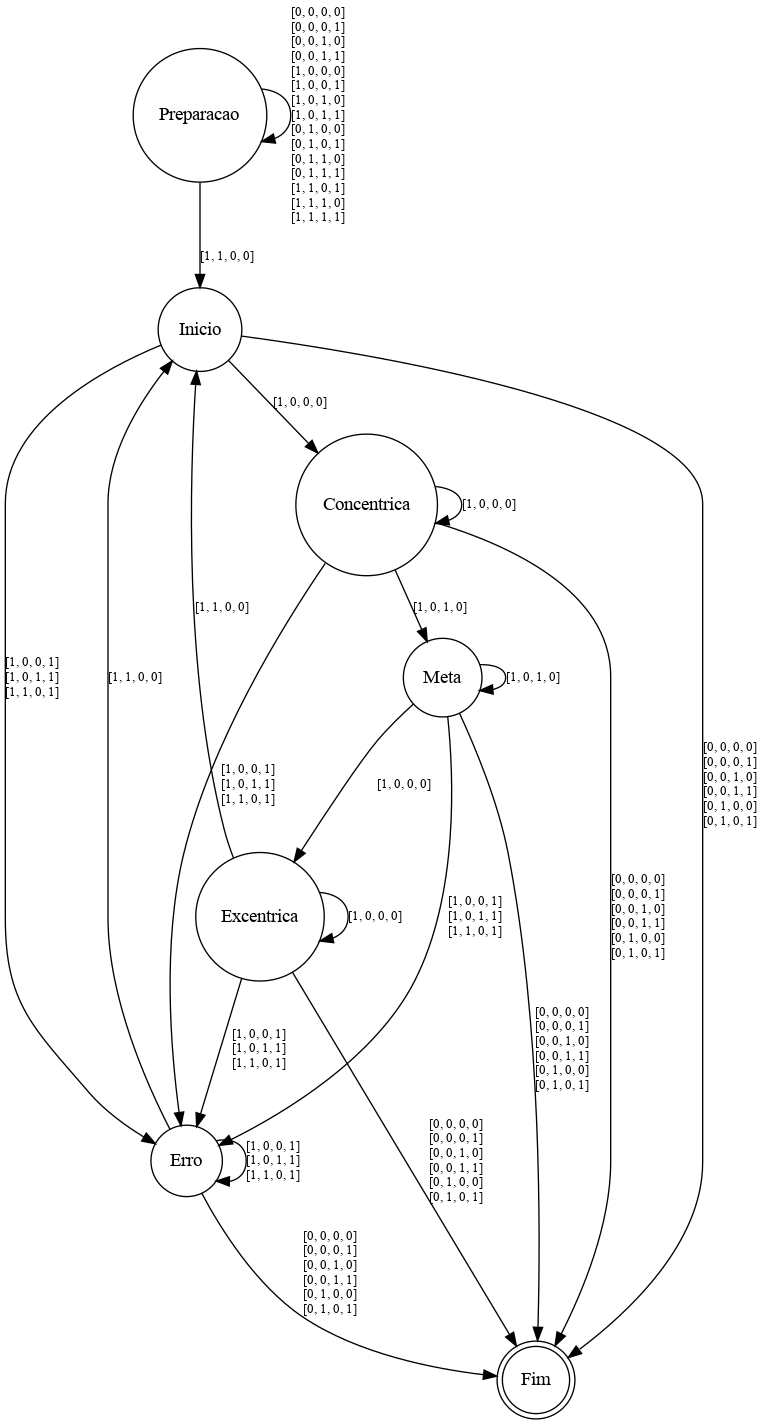
\includegraphics[scale=0.4]{figuras/AFD/afd_barra.png}
    \legend{Fonte: Elaborado pelo autor (2023)}
	\label{fig:transicaoAFD}
\end{figure}


\section[Extração de informação frame a frame]{Extração de informação frame a frame}\label{sec:Extracao de informacao frame a frame}

Dentro do processamento de imagem, a segmentação é a etapa onde a imagem é dividida em regiões ou componentes significativos que podem ser analisados e processados de forma independente. Em outras palavras, a segmentação visa identificar áreas distintas na imagem que correspondem a objetos, padrões, bordas ou características de interesse \cite{imagemMonocromatica}.

O objetivo da ferramenta é operar em um ambiente controlado. Entretanto, devido às características específicas da infraestrutura do local de teste, tornou-se essencial incorporar uma máscara para uma manipulação adequada de cada quadro. Com esse propósito, uma máscara previamente elaborada a partir do primeiro quadro do vídeo foi aplicada, utilizando a função bitwise\_and, disponibilizada na biblioteca \ac{openCV}. A operação bitwise\_and consiste em um processo de AND bit a bit entre os valores dos pixels do quadro e os valores correspondentes da máscara. O resultado é uma nova imagem em que os pixels que não fazem parte das regiões brancas da máscara são convertidos para preto, enquanto os pixels que pertencem a essas regiões permanecem intactos. A finalidade dessa máscara é realçar a região de interesse dentro do quadro, permitindo um foco preciso durante a etapa de segmentação da imagem.
\begin{figure}[htb]
    \centering
    \caption{Ambiente de gravação e Mascara Preto e Branca criada apartir do mesmo}
        \begin{minipage}{0.4\textwidth}
            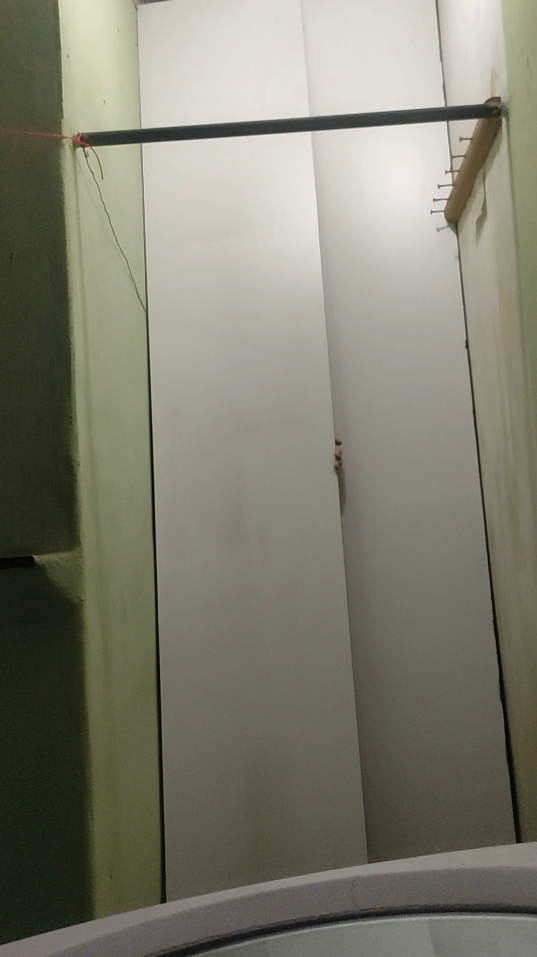
\includegraphics[width=\textwidth]{figuras/filter/mask/ambiente.png}
        \end{minipage}
        \begin{minipage}{0.4\textwidth}
            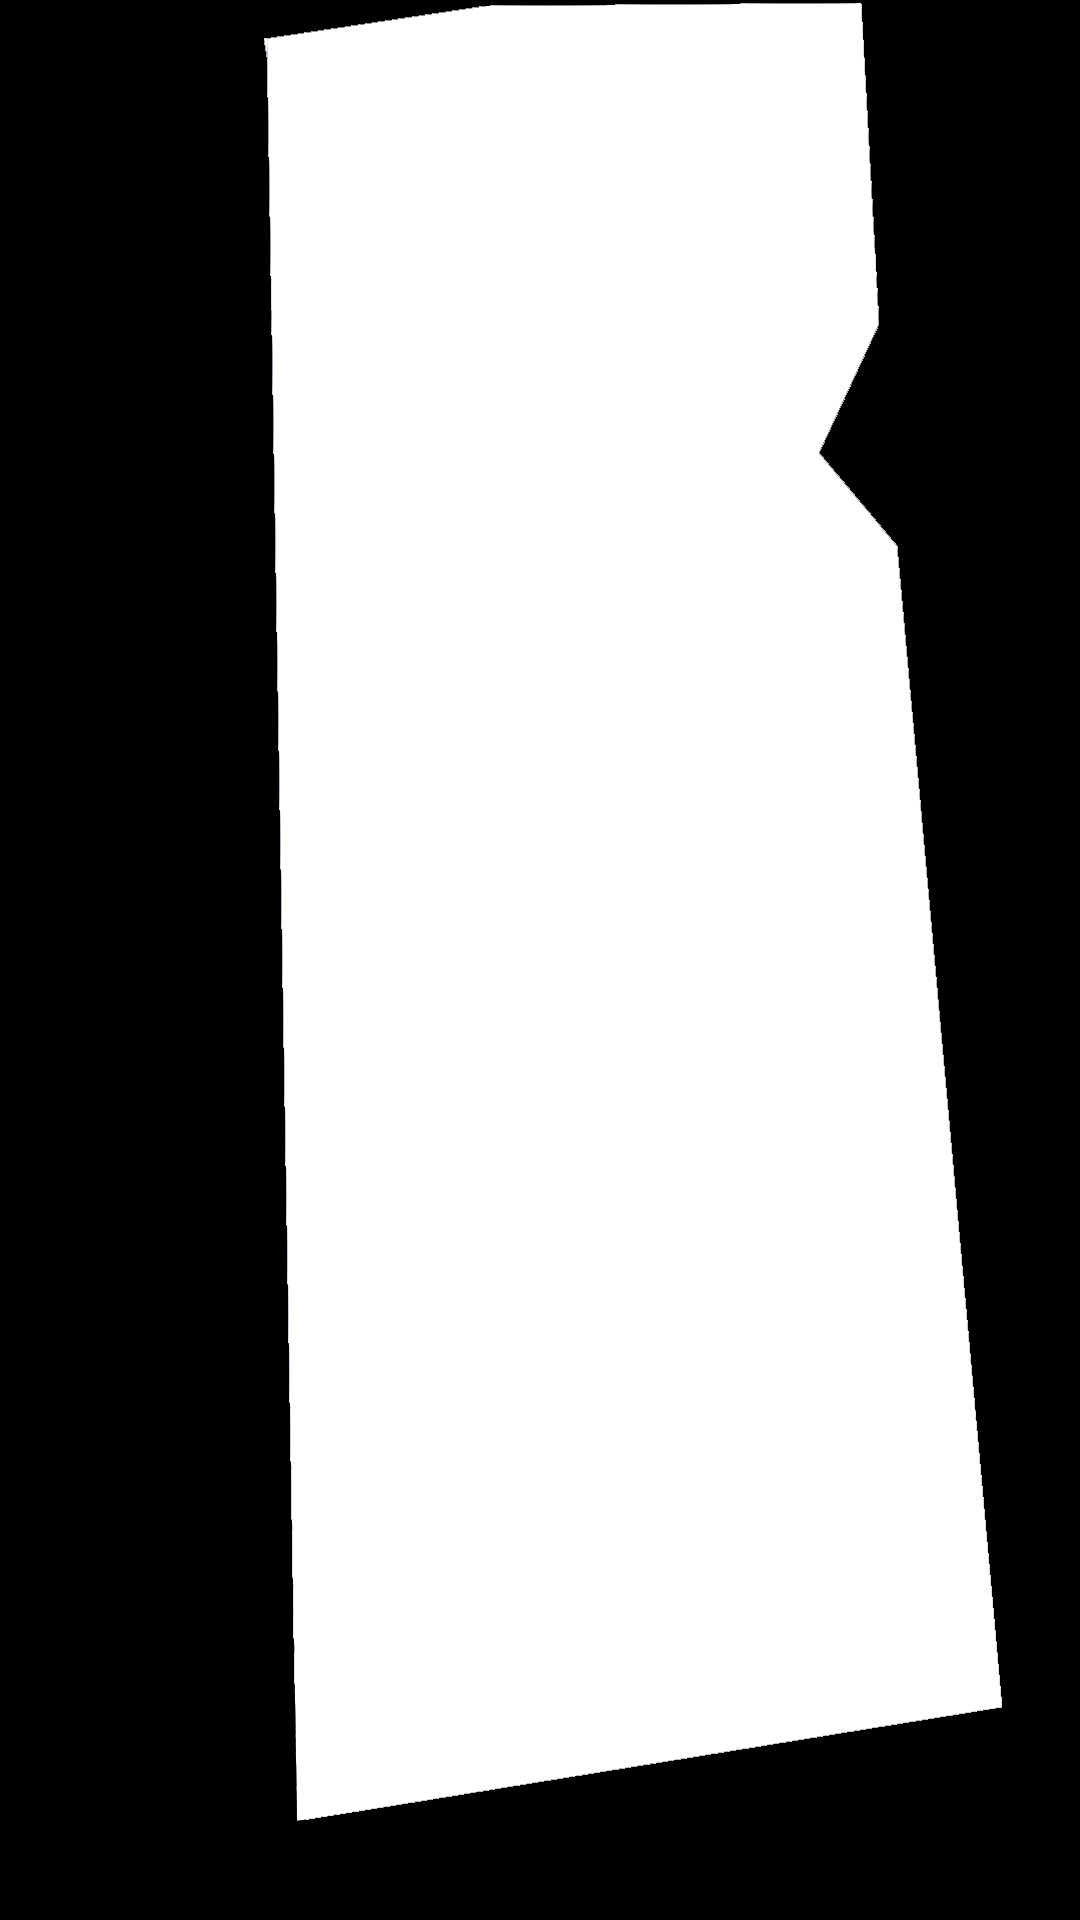
\includegraphics[width=\textwidth]{figuras/filter/mask/mask.png}
        \end{minipage}
    \legend{Fonte: Elaborado pelo autor (2023)}
    \label{fig:maskAmbiente}
\end{figure}

\subsection[Detecção da barra]{Detecção da barra}\label{sec:Deteccao da barra}

Para a detecção da barra fixa, foi empregado o filtro de Canny \ref{sec:Detector de bordas de Canny} com o intuito de mitigar ruídos e enfatizar as bordas proeminentes. Para essa finalidade, foi adotada a função incorporada à biblioteca \ac{openCV}, sendo parametrizada da seguinte forma: o limite inferior do processo de histerese foi estabelecido em 50, o limite superior definido em 100, e o tamanho do kernel aplicado ao operador Sobel foi estipulado como 3. 

Após a etapa de pré-processamento da imagem, foi empregada a Transformada de Hough \ref{sec:Transformada de Hough}, também disponibilizada na biblioteca \ac{openCV}. Essa aplicação foi configurada com os seguintes parâmetros: a resolução da distância no acumulador, em pixels, foi definida como 1; a resolução angular no acumulador, em radianos, foi estabelecida em $\pi$/180, equivalente a 1 grau; e o limiar do acumulador foi fixado em 150. Essas configurações asseguram a avaliação de cada pixel para sua inclusão ou não como parte de uma reta, além de garantir uma inclinação mínima de 1º de uma reta a outra e que sejam consideradas retas apenas aquelas que tiverem 150 votos ou mais contabilizados no acumulador.

\begin{figure}[htb]
    \centering
        \caption{Aplicação do filtro de Canny.}
        \begin{minipage}{0.45\textwidth}
            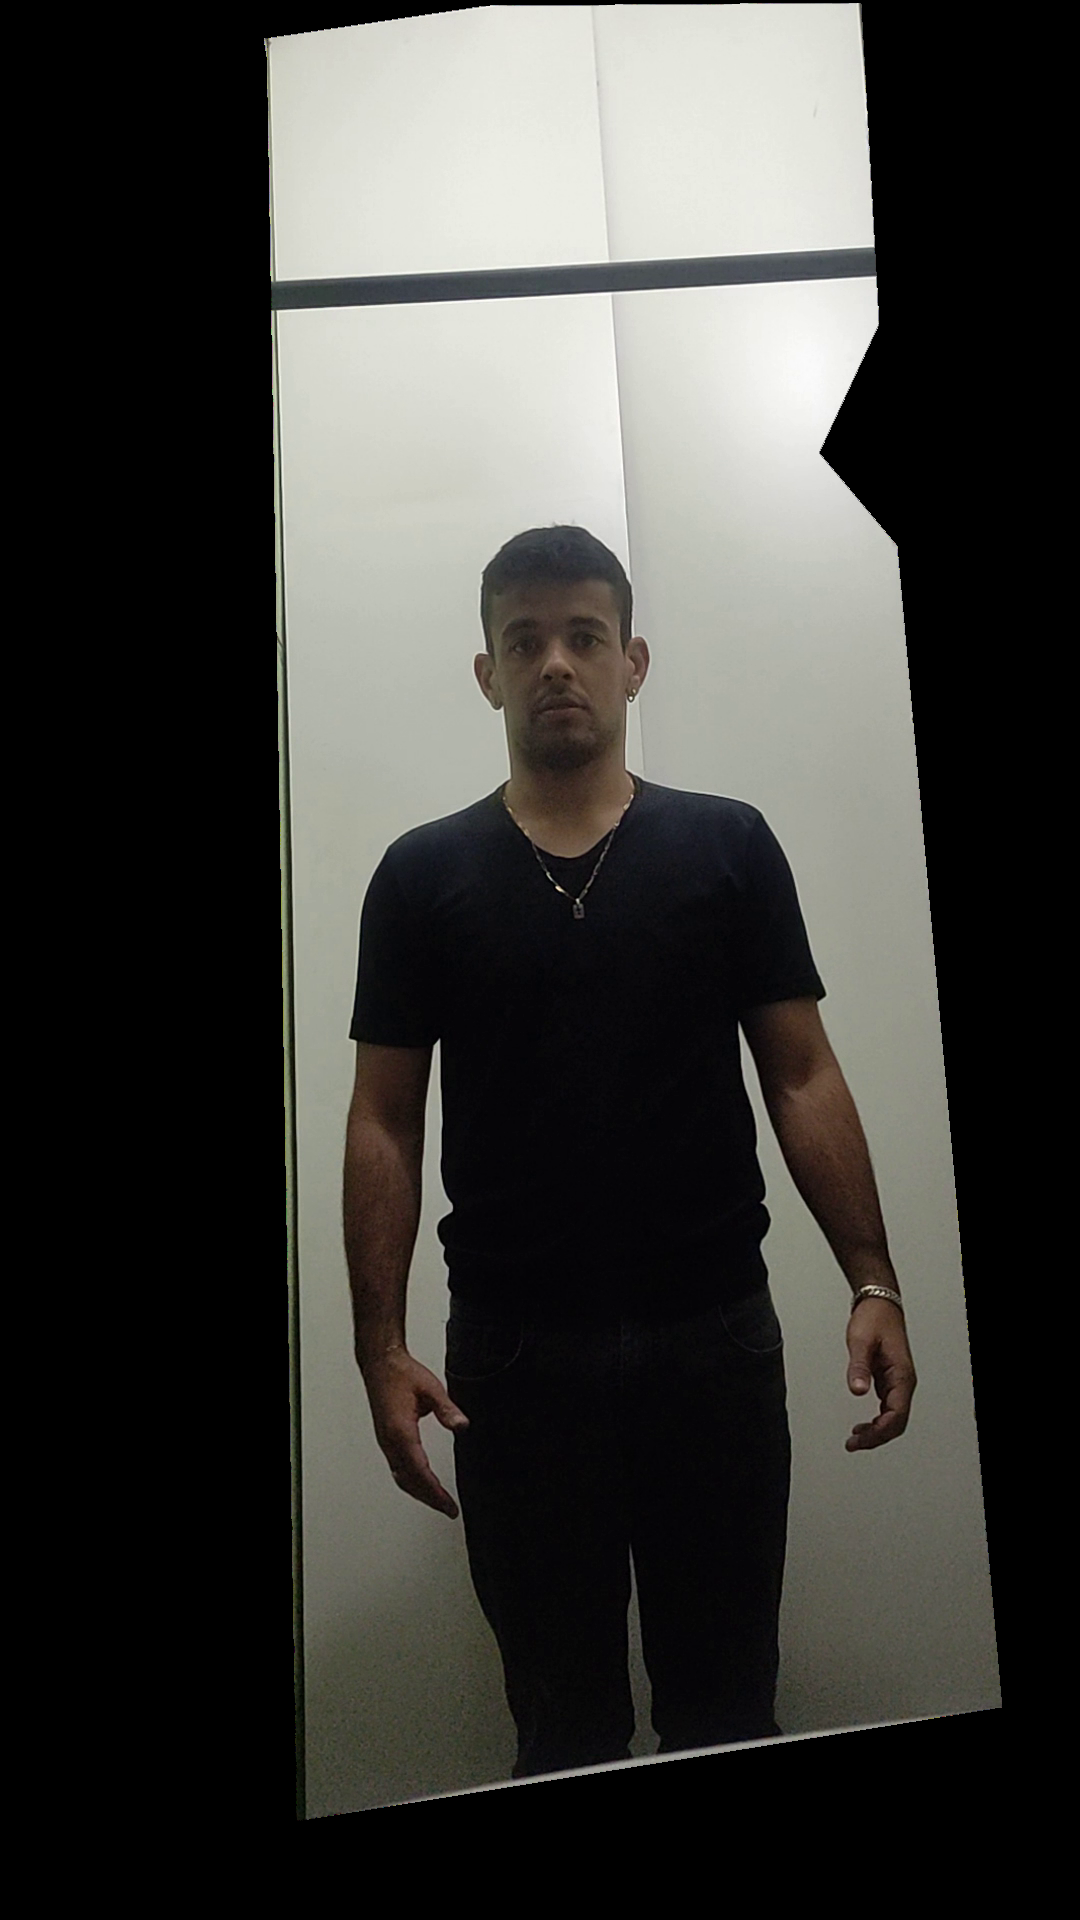
\includegraphics[width=\textwidth]{figuras/filter/canny/mask.png}
        \end{minipage}
        \begin{minipage}{0.45\textwidth}
            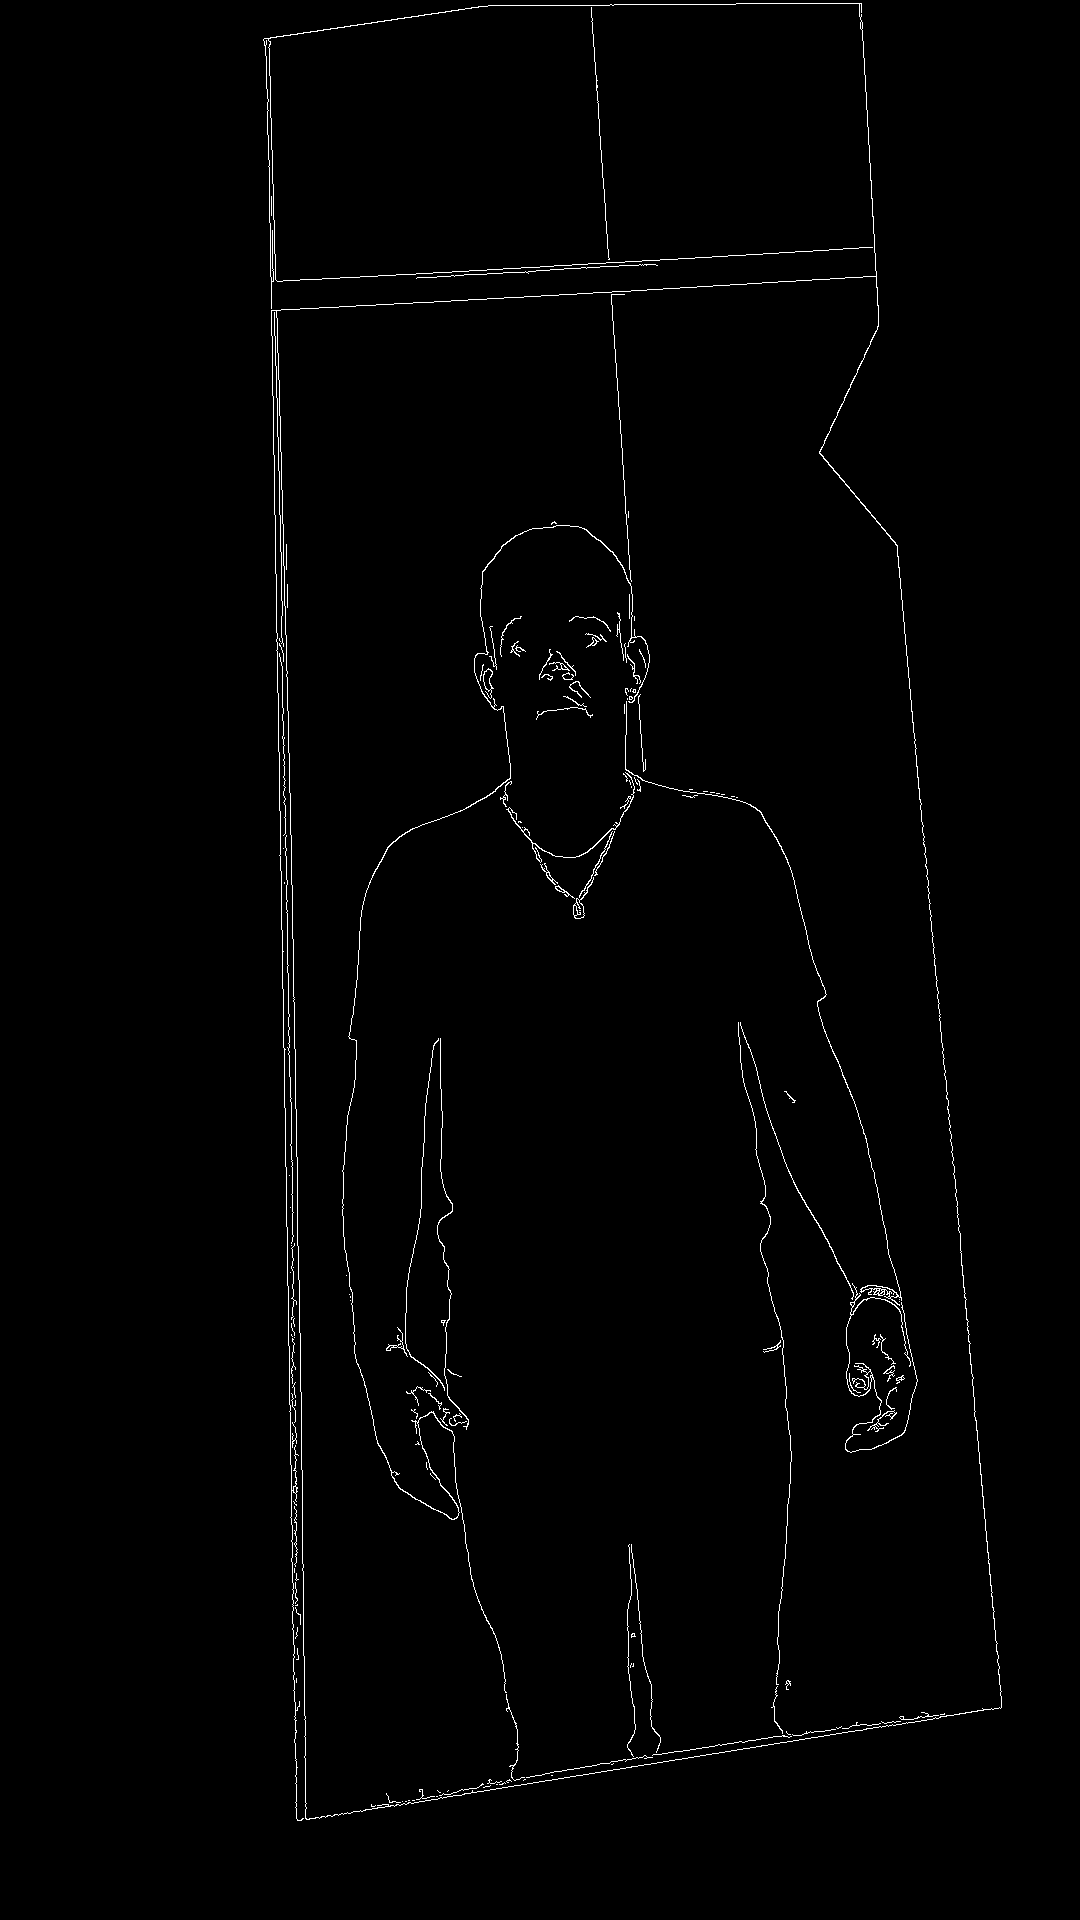
\includegraphics[width=\textwidth]{figuras/filter/canny/canny.png}
        \end{minipage}
    \legend{Fonte: Elaborado pelo autor (2023)}
    \label{fig:maskCanny}
\end{figure}

O resultado da Transformada de Hough \ref{sec:Transformada de Hough} foi filtrado, selecionando apenas retas horizontais com uma tolerância de 10°, ou seja, somente retas cujo valor absoluto do ângulo é menor que o valor da tolerância, ou ainda, cujo valor absoluto da diferença entre 180 e a tolerância é menor que o valor absoluto do ângulo.

Após a etapa inicial de filtragem, uma segunda filtragem foi aplicada para selecionar exclusivamente as retas localizadas em uma região específica do \textit{frame}. Essa região é demarcada como a porção superior, correspondendo a 30\% da área total. Essa abordagem foi adotada com base na expectativa de que a barra esteja consistentemente posicionada na parte superior do vídeo, uma vez que é crucial capturar o corpo estendido na barra e a parte dele que ultrapassa a barra.

Por meio dessa abordagem, a expectativa era identificar duas retas paralelas que representassem a seção superior e inferior da barra. Como desenvolvimento, as duas retas com maior número de votos foram selecionadas, e procedeu-se à determinação do ponto médio das coordenadas $y$ entre elas no sistema cartesiano $(x, y)$. Nesse contexto, a barra foi concebida como uma reta paralela às outras duas, passando pelo ponto médio das coordenadas $y$ correspondentes a essas retas.

A cada quadro, o procedimento de detecção da barra é repetido. Para lidar com \textit{frames} em que a barra não é detectada e minimizar a variação na posição da barra devido a flutuações na iluminação ou tremores no vídeo, os valores representativos da barra são acumulados. Em outras palavras, a cada nova detecção, os valores $(x,y)$ que representam o início e o fim da barra são acumulados em quatro variáveis, aqui denominadas como ($x_{\text{start}}, y_{\text{start}}$) e ($x_{\text{end}}, y_{\text{end}}$). O valor de $x$ que representa a posição $x$ correspondente ao início da barra atual é definido como o valor acumulado na variável $x_{\text{start}}$, dividido pela quantidade de \textit{frames} processados. O mesmo princípio é aplicado às outras coordenadas da barra. Esse método ajuda a suavizar a posição da barra ao longo do tempo, tornando-a menos suscetível a flutuações abruptas e permitindo uma estimativa mais estável da sua posição real.

É esperado que não haja muita variação na detecção da barra, mas mesmo assim, ao longo do tempo, o valor da barra tende a convergir a um ponto central. Quanto mais tempo passa, melhor fica a inferência da barra quando ela não consegue ser detectada.

O processo pode ser visualizado no diagrama a seguir.


\begin{figure}[H]
	\centering
    \caption{Diagrama do processo de detecção da barra}
	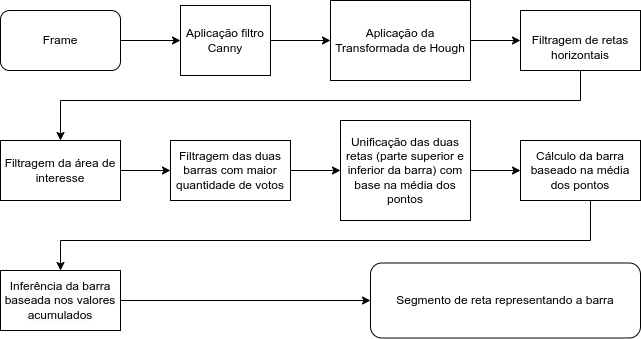
\includegraphics[scale=0.6]{figuras/diagrama/detectar barra.png}
    \legend{Fonte: Elaborado pelo autor (2023)}
	\label{diagrama:Detectar barra}
\end{figure}


\subsection[Inclinação da barra]{Inclinação da barra}\label{sec:Inclinacao da barra}

Durante o exame da barra física, é necessário que a barra esteja alinhada de forma paralela ao solo. Contudo, devido a um possível posicionamento inadequado da câmera, o vídeo pode demonstrar uma inclinação na barra. Para corrigir isso, o ângulo de inclinação da barra é calculado e, posteriormente, o frame é rotacionado de acordo com essa inclinação. Essa ação tem como objetivo assegurar que, na imagem, a barra se torne paralela à base da imagem, alinhando-a de forma apropriada em relação ao plano horizontal.

\begin{figure}[H]
	\centering
	\caption{Imagem rotacionada em relação a barra}
	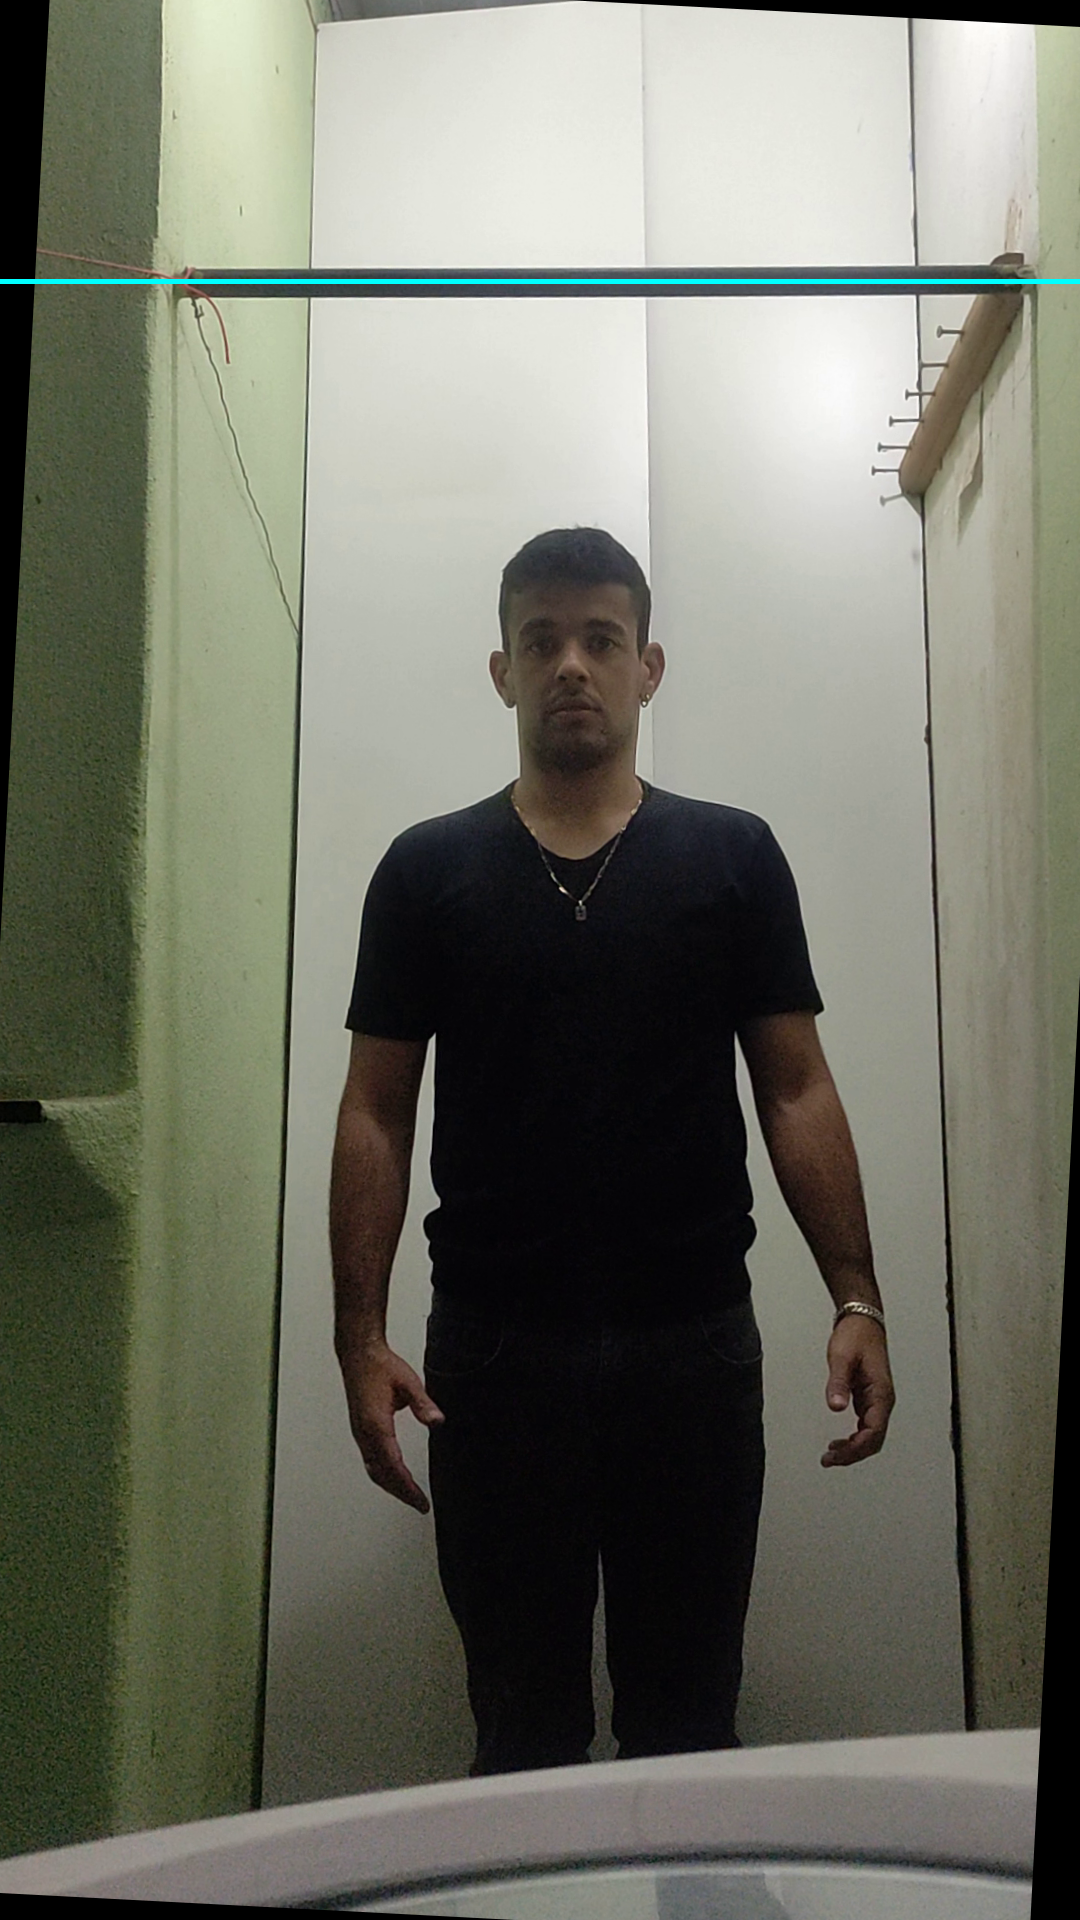
\includegraphics[scale=0.12]{figuras/processo/detectarBarra/barra_rotacionada.png}
    \legend{Fonte: Elaborado pelo autor (2023)}
	\label{fig:Barra rotacionada}
\end{figure}




\subsection[Reconhecimento de pose humana]{Estimativa de pose humana}\label{sec:Reconhecimento de pose humana}

Foi adotada a biblioteca MediaPipe como uma ferramenta crucial para a predição dos pontos de referência da pose humana a partir de frames. Durante a configuração da ferramenta, foram considerados quatro de sete parâmetros para otimizar o desempenho do sistema: $static\_image\_mode$, $model\_complexity$, $min\_detection\_confidence$ e $min\_tracking\_confidence$. Cada um desses parâmetros desempenha um papel fundamental na precisão e eficiência da \ac{EPH}, contribuindo para a robustez e a qualidade dos resultados obtidos em nosso estudo.

O parâmetro $static\_image\_mode$ pode ser configurado como $False$ ou $True$. Esse parâmetro determina se as imagens de entrada serão tratadas como um fluxo contínuo de vídeo ou como imagens independentes. Quando $static\_image\_mode$ é definido como $False$, o sistema realiza uma detecção inicial para identificar a pessoa mais proeminente. Após essa detecção, ocorre o \textit{tracking} dos pontos de referência, evitando a necessidade de iniciar uma nova detecção a cada quadro subsequente, a menos que o ponto de referência seja perdido. Por outro lado, quando $static\_image\_mode$ é configurado como $True$, o sistema processa um lote de imagens como entidades independentes e não relacionadas. A cada nova detecção, os valores anteriores são descartados, e todo o processo é reiniciado.

No contexto do nosso projeto, optamos por configurar o $static\_image\_mode$ como $False$, aproveitando a eficiência proporcionada pelo rastreamento contínuo de pontos de referência. Isso contribui para melhorar a computação geral e reduzir a latência do processo. Essa escolha foi feita com base nas necessidades específicas de nossa aplicação.

O parâmetro $model\_complexity$ pode ser configurado com os valores predefinidos $0$, $1$ e $2$ e está ligado à precisão do ponto de referência. Quanto maior o número, maior a complexidade, influenciando diretamente a latência de inferência. Foi utilizado o valor $2$ porque os demais valores estavam gerando inferências errôneas em frames específicos, o que impactava diretamente na extração de características desses frames.

O parâmetro $min\_detection\_confidence$ pode ser configurado como um valor entre $0.0$ a $1.0$ e define o valor de confiança mínimo para que o modelo de detecção de pessoa seja considerado bem-sucedido. O valor adotado foi $0.3$.

O parâmetro $min\_tracking\_confidence$ pode ser configurado como um valor entre $0.0$ a $1.0$ e define o valor de confiança mínimo para que o modelo de rastreamento de pontos seja considerado rastreado com sucesso. O valor adotado foi $0.75$. Configurá-lo com um valor mais alto pode aumentar a robustez da solução, às custas de uma latência mais alta.

A biblioteca MediaPipe fornece 33 pontos de referência, como mostrado na Figura \ref{fig:Pontos de referencia}. No entanto, foram utilizados apenas 16 pontos, sendo eles:

\begin{itemize}
    \item[11] - ombro esquerdo
    \item[12] - ombro direito
    \item[13] - cotovelo esquerdo
    \item[14] - cotovelo direito
    \item[15] - pulso esquerdo
    \item[16] - pulso direito
    \item[17] - mindinho esquerdo
    \item[18] - mindinho direito
    \item[19] - indicador esquerdo
    \item[20] - indicador direito
    \item[23] - quadril esquerdo
    \item[24] - quadril direito
    \item[25] - joelho esquerdo
    \item[26] - joelho direito
    \item[29] - calcanhar esquerdo
    \item[30] - calcanhar direito
\end{itemize}

\newpage
Podendo ser representado na figura a seguir:

\begin{figure}[H]
	\centering
	\caption{Pontos de referência usados na aplicação}
	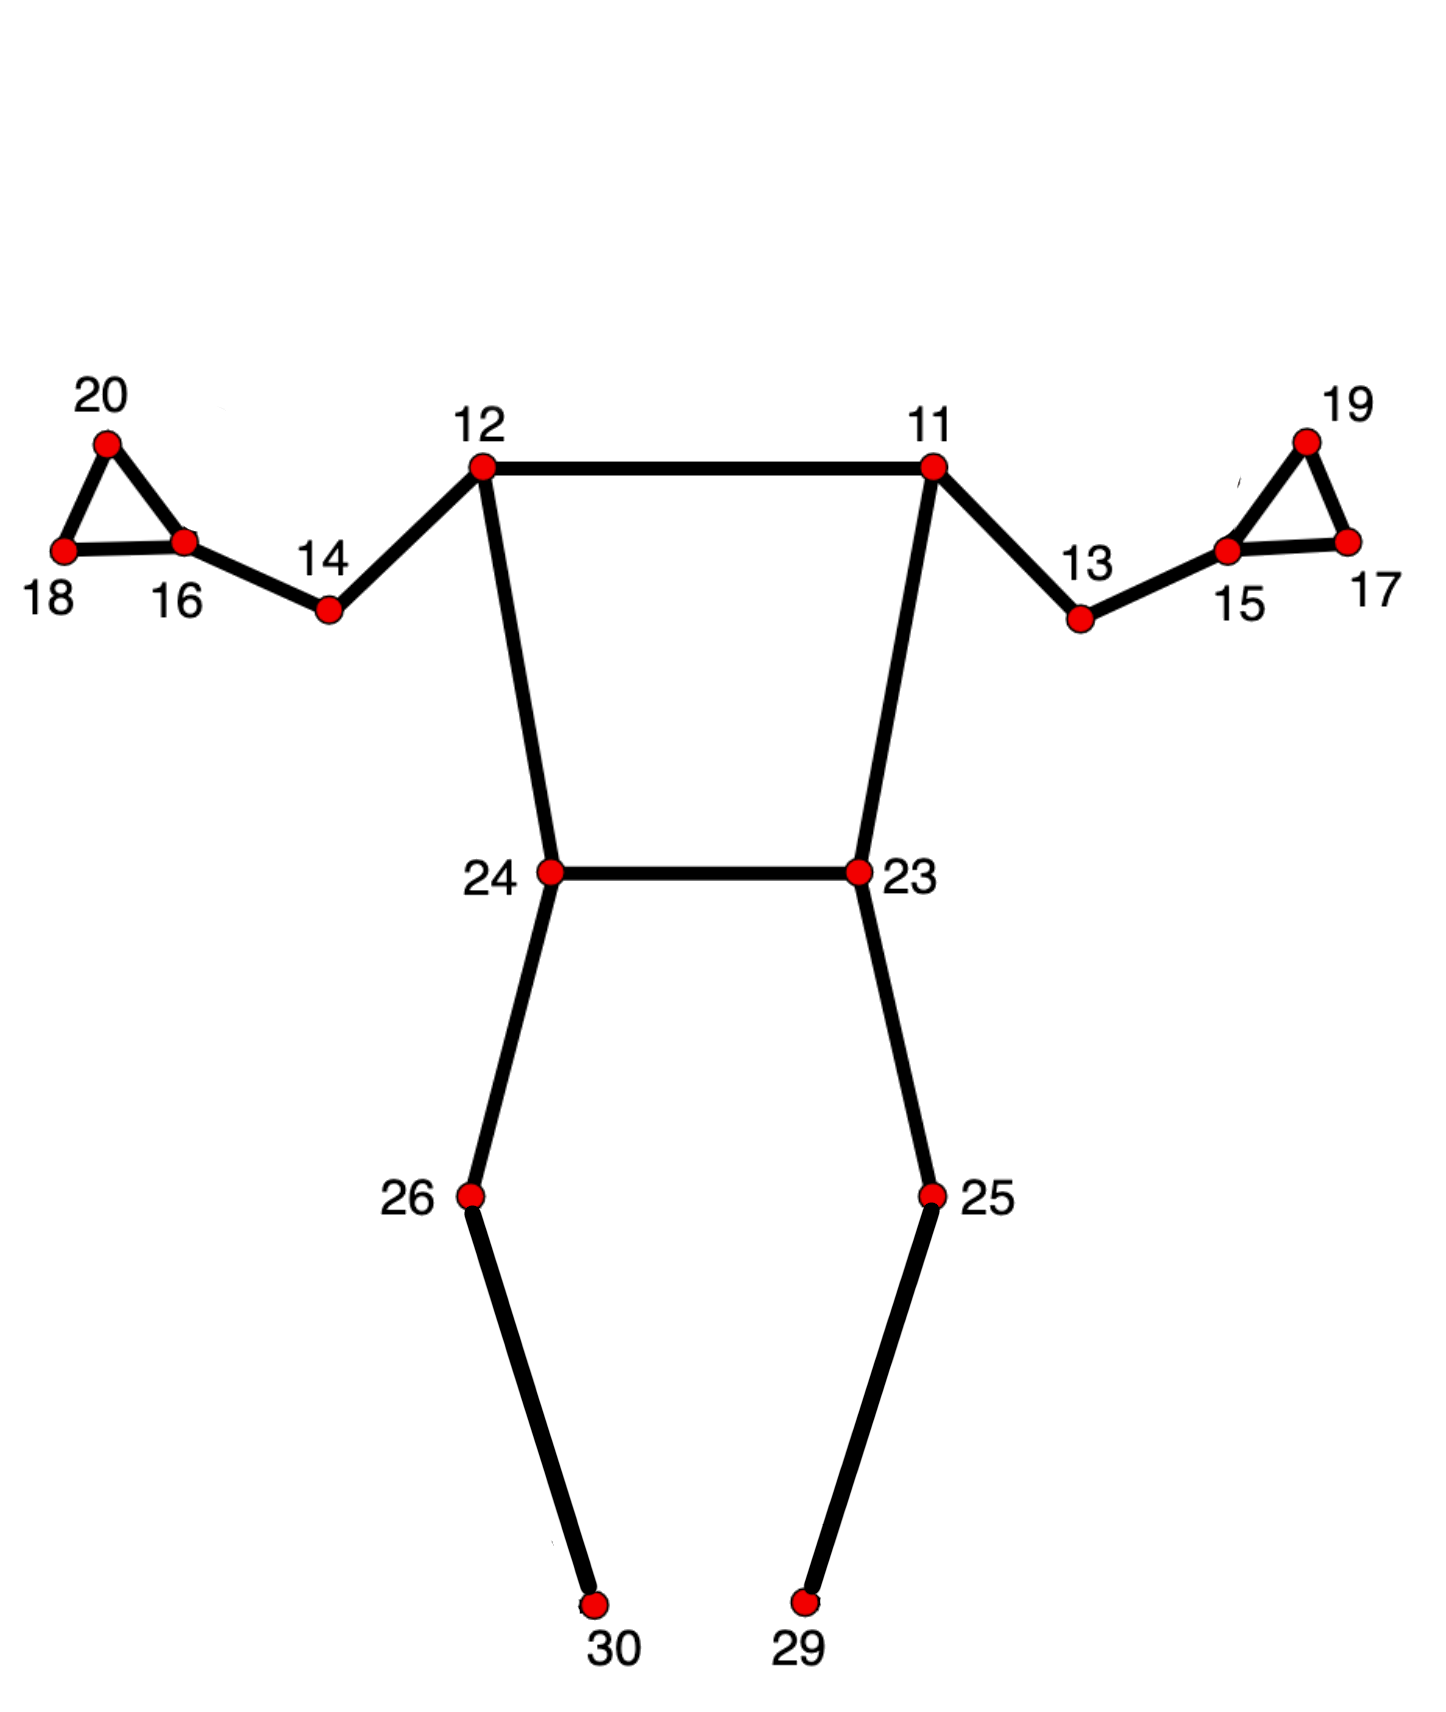
\includegraphics[scale=0.2]{figuras/eph/pose_landmarks_custom.png}
    \legend{Fonte: Elaborado pelo autor (2023) baseado na Figura \ref{fig:Pontos de referencia}}
	\label{fig:Pontos de referencia usados na aplicacao}
\end{figure}

\subsection[Mão na barra]{Mão na barra}\label{sec:Mao na barra}


Para realizar a detecção das mãos na barra, foi seguida uma sequência de etapas bem definidas. Inicialmente, foi aplicada uma máscara que identificou os pixels na imagem que estavam dentro do intervalo de cor (0, 25, 0) a (20, 255, 255). Enquanto os outros pixels foram definidos como pretos, destacando assim a cor da pele do executor.

\renewcommand{\sizeImg}{0.3}
\begin{figure}[H]
    \caption{Filtragem pela cor de pele}
    \centering
        \begin{minipage}{\sizeImg\textwidth}
            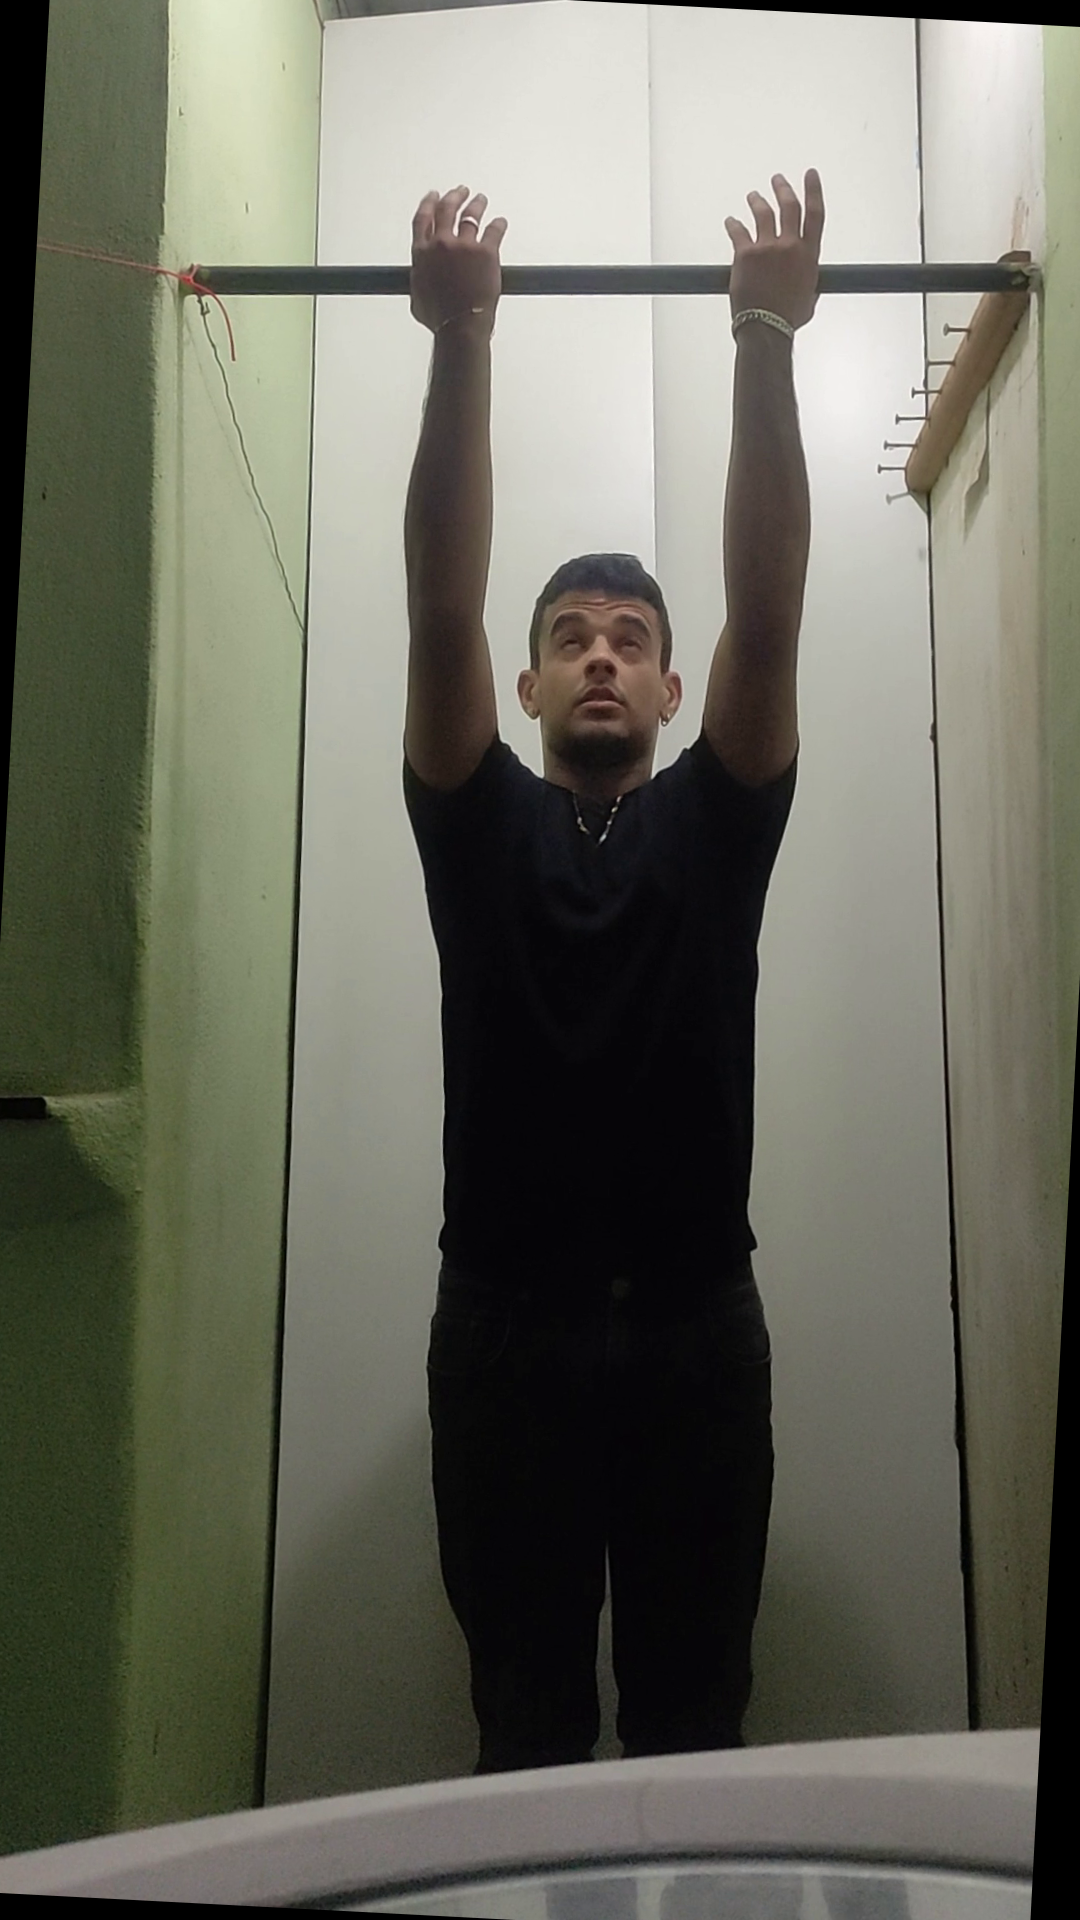
\includegraphics[width=\textwidth]{figuras/mao_barra/original.png}
        \end{minipage}
        \begin{minipage}{\sizeImg\textwidth}
            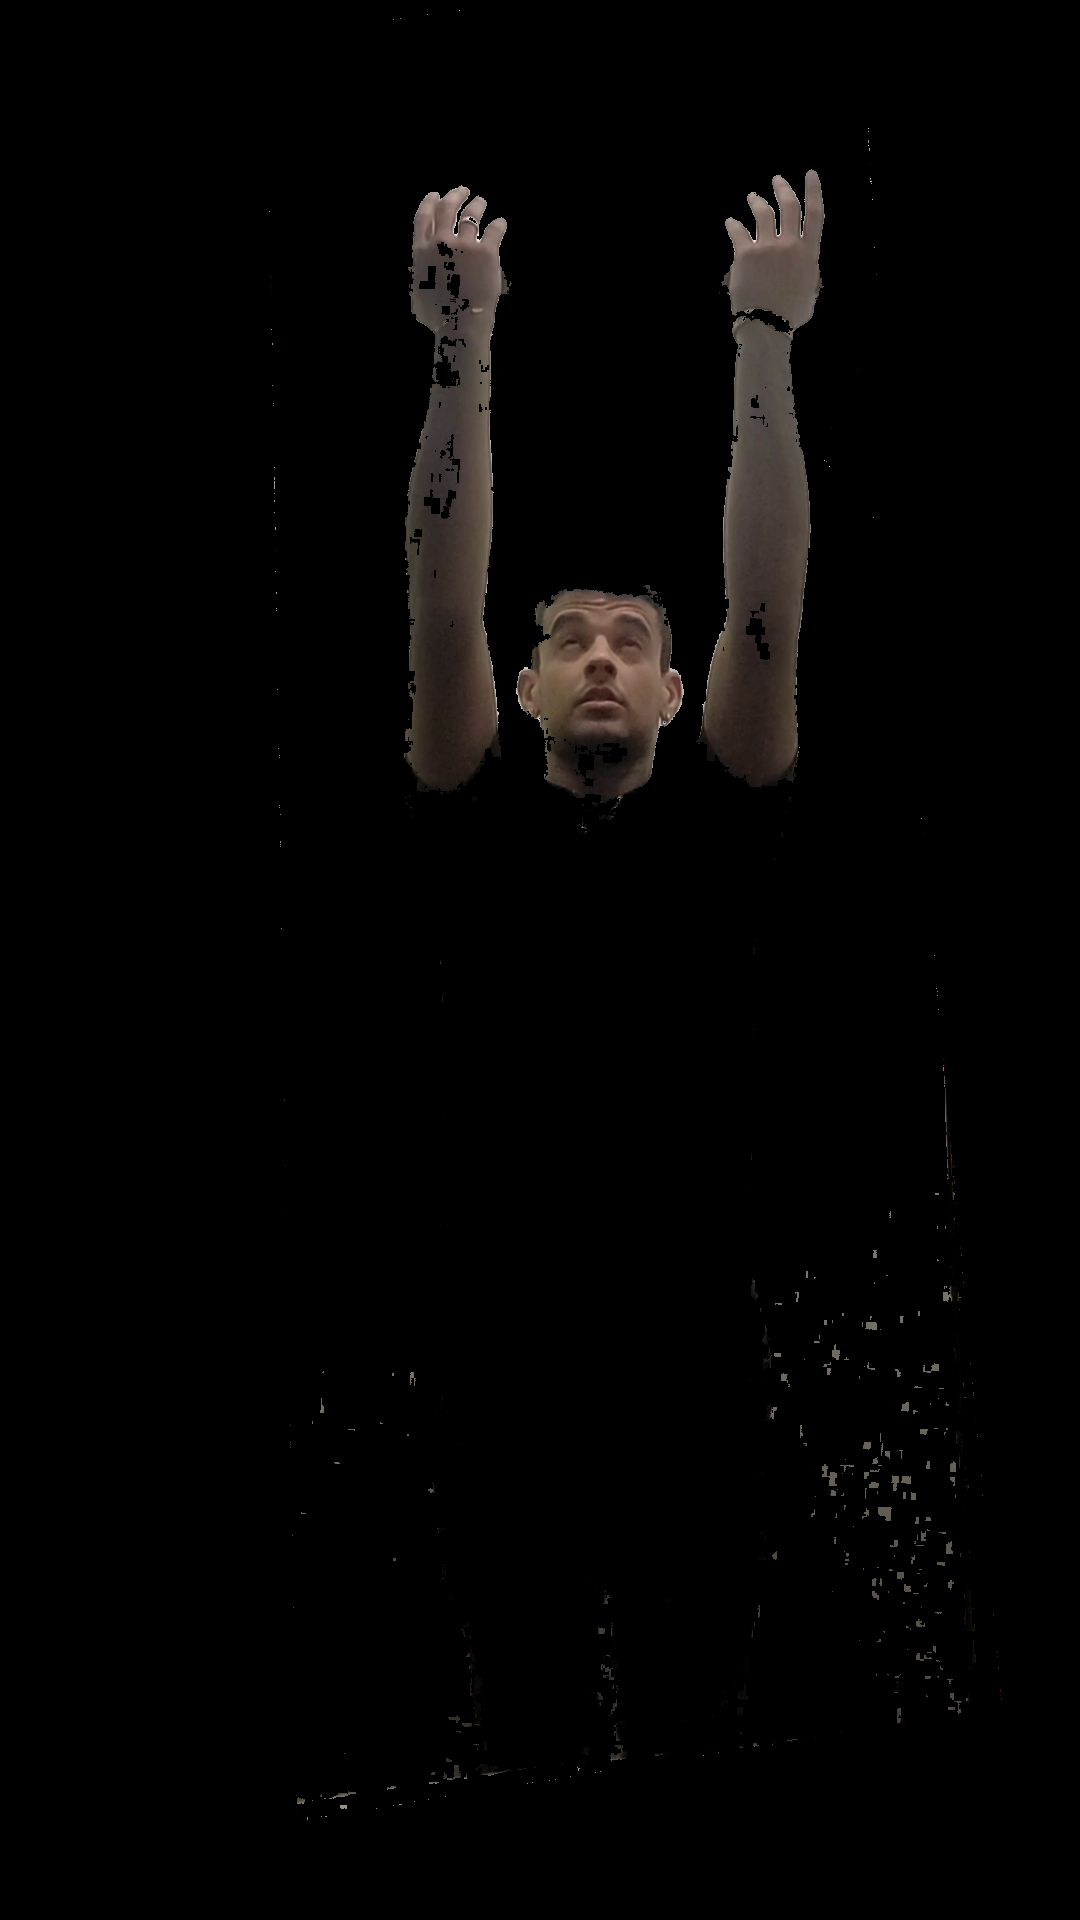
\includegraphics[width=\textwidth]{figuras/mao_barra/skin.png}
        \end{minipage}
    \legend{Fonte: Elaborado pelo autor (2023)}
    \label{fig:skin}
\end{figure}

Posteriormente, a imagem que estava em \ac{RGB} foi convertida para um único canal por meio da função $cvtColor$ presente na biblioteca \ac{openCV}. Foi utilizada a constante $COLOR\_BGR2GRAY$ da própria biblioteca, convertendo os três canais (Azul, Verde e Vermelho) para uma escala de cinza.

\begin{figure}[H]
    \centering
    \caption{Conversão em escala de cinza}
        \begin{minipage}{\sizeImg\textwidth}
            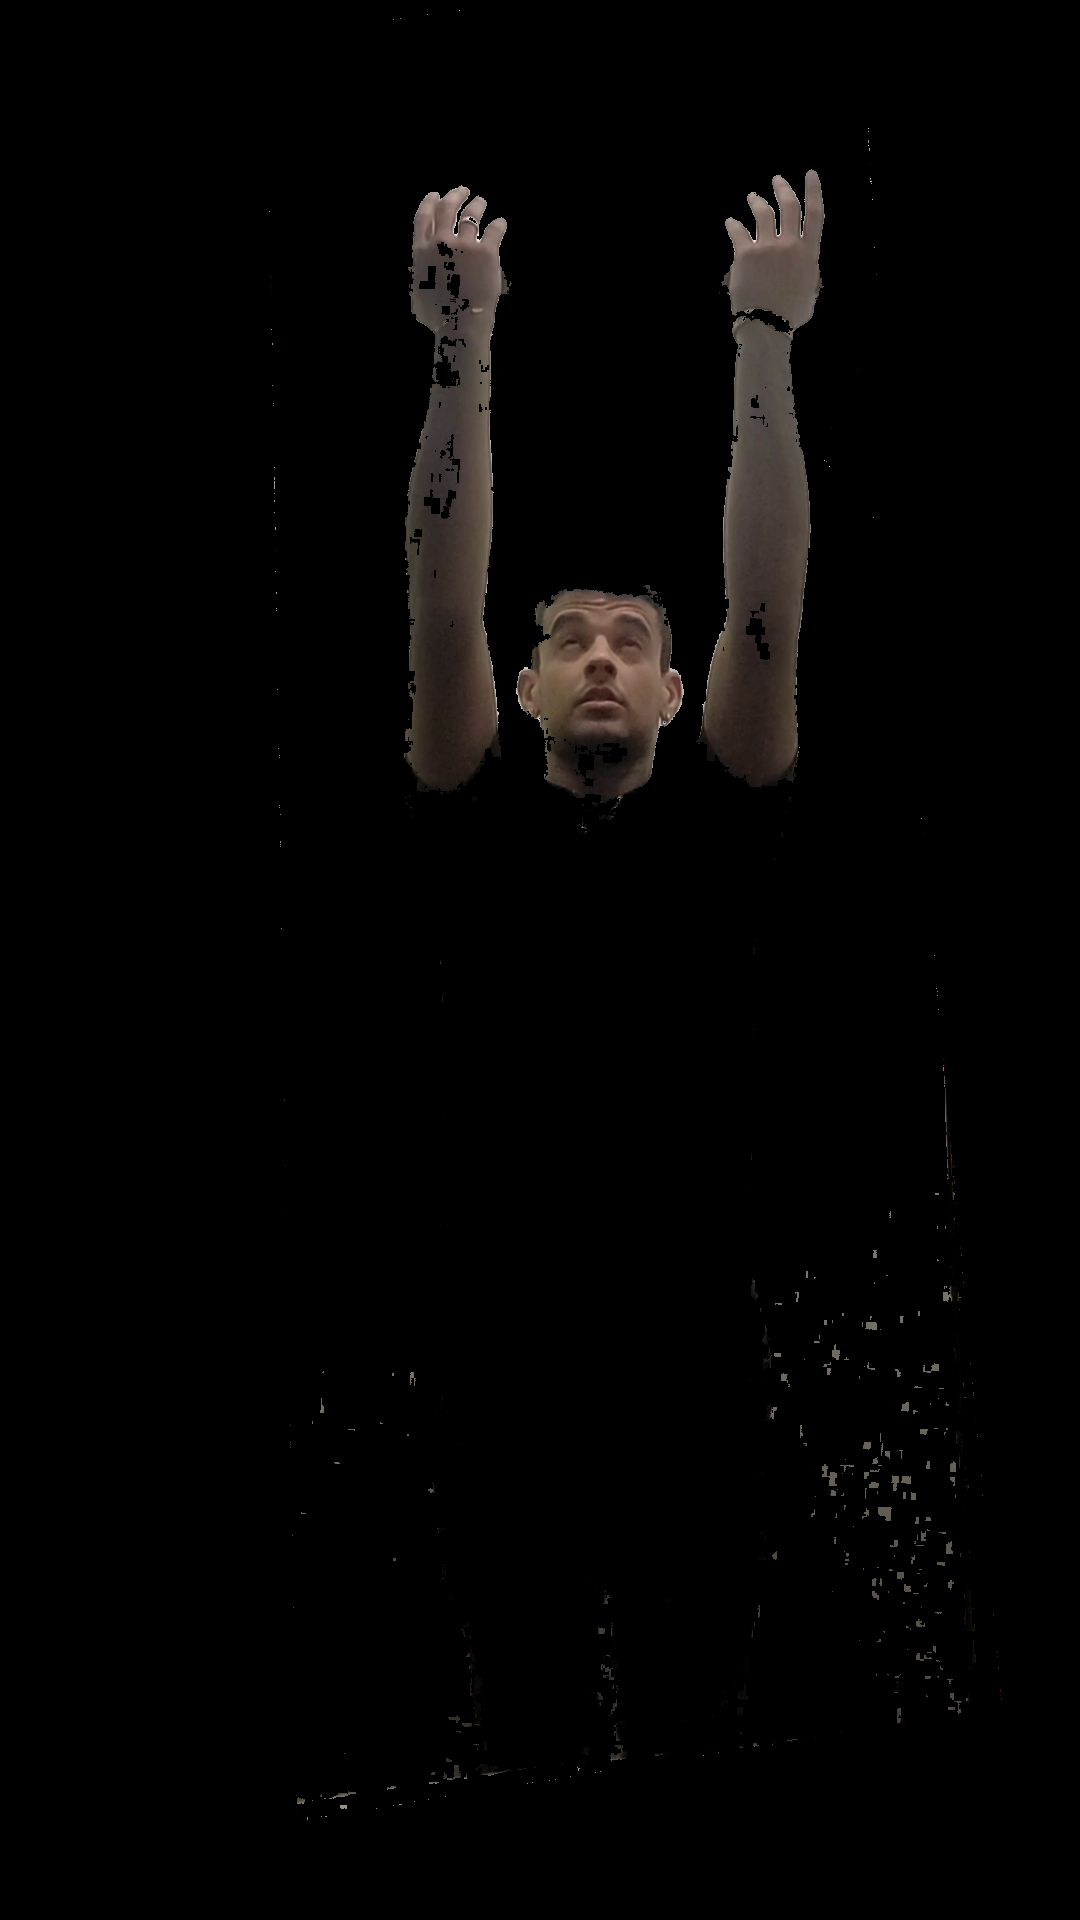
\includegraphics[width=\textwidth]{figuras/mao_barra/skin.png}
        \end{minipage}
        \begin{minipage}{\sizeImg\textwidth}
            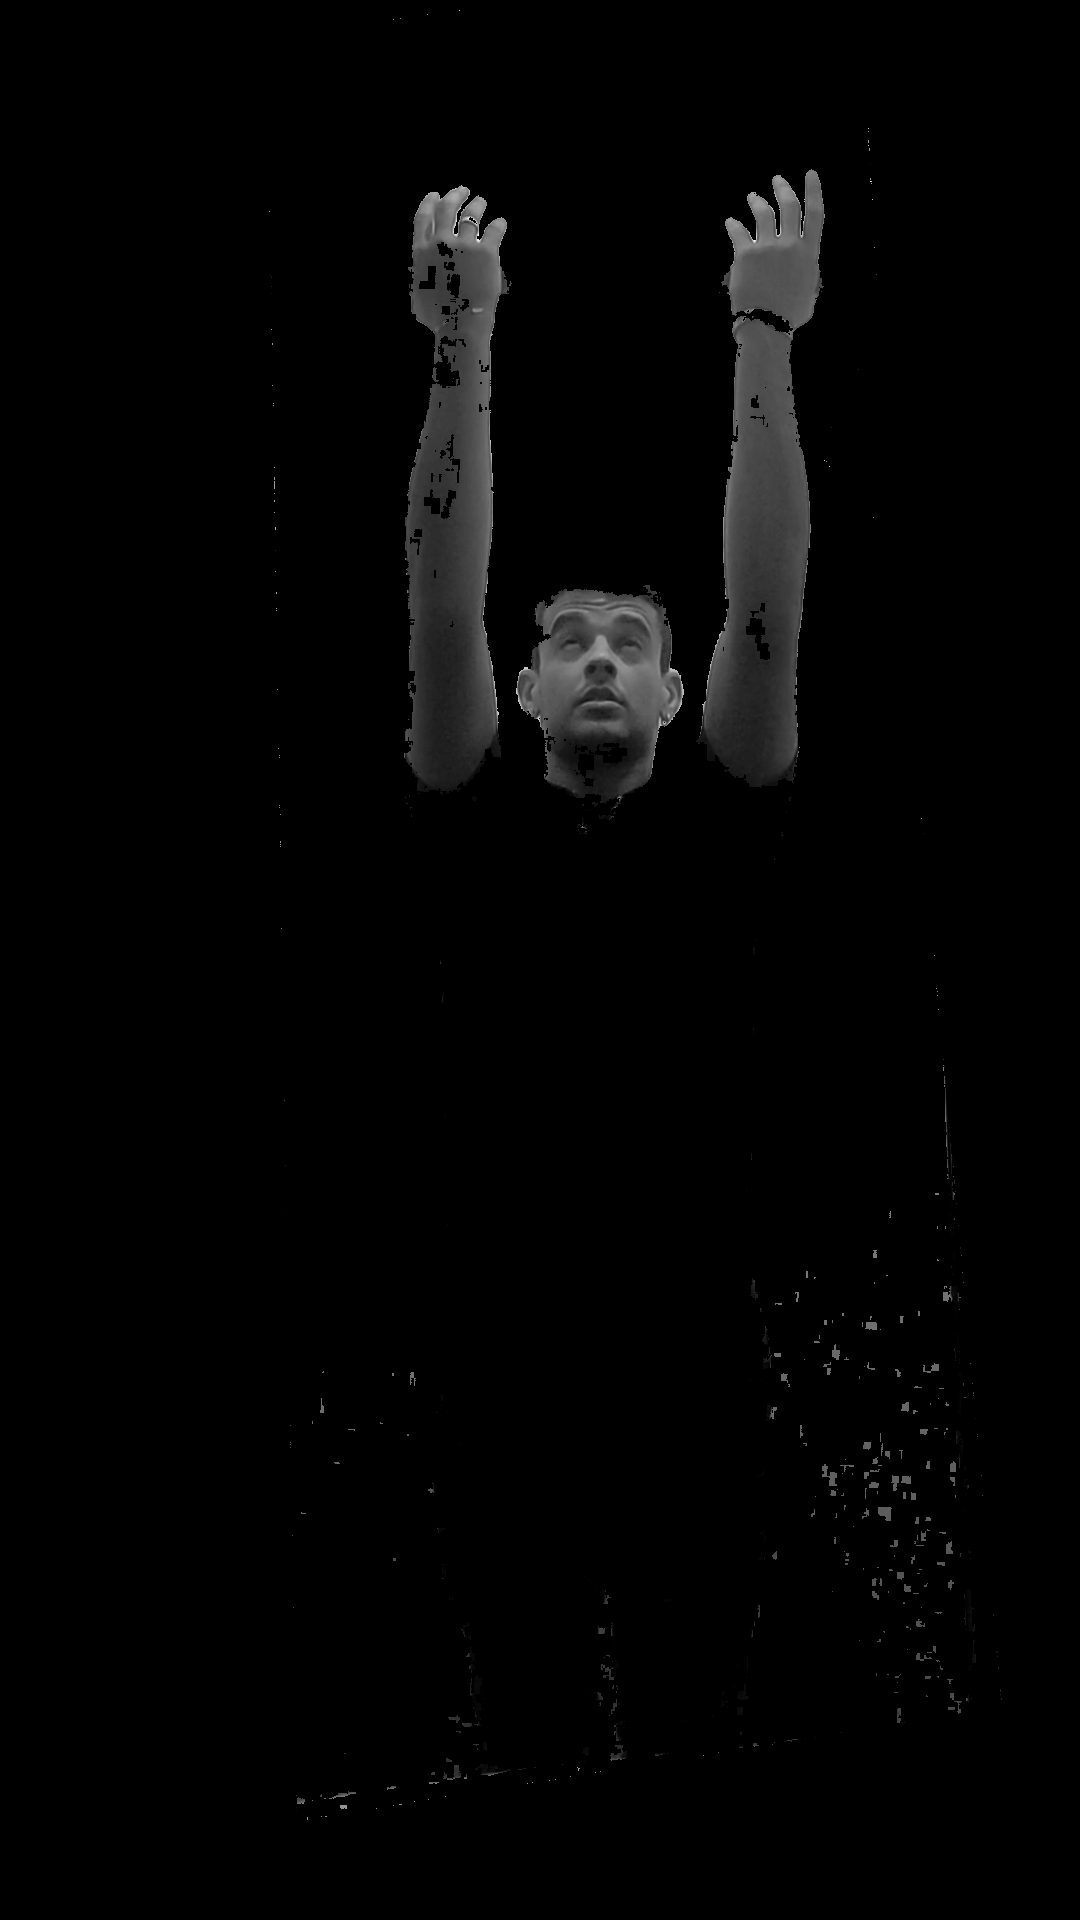
\includegraphics[width=\textwidth]{figuras/mao_barra/gray.png}
        \end{minipage}
    \legend{Fonte: Elaborado pelo autor (2023)}
    \label{fig:gray}
\end{figure}

A partir desse ponto, a imagem passa a conter diferentes níveis de brilho, representados em uma escala de cinza. Foi aplicado um filtro de limiarização da biblioteca \ac{openCV}, utilizando a função $threshold$ com a constante $THRESH\_BINARY$ e o valor de limiar 50 como parâmetros. Nesse processo, todos os pixels com valores iguais ou superiores a 50 foram convertidos para o valor 255, enquanto os pixels com valores menores foram convertidos para o valor 0. Isso resultou em uma imagem binarizada que tem o propósito de representar a presença ou ausência do executor.

\begin{figure}[H]
    \centering
    \caption{Binarização da Imagem}
        \begin{minipage}{\sizeImg\textwidth}
            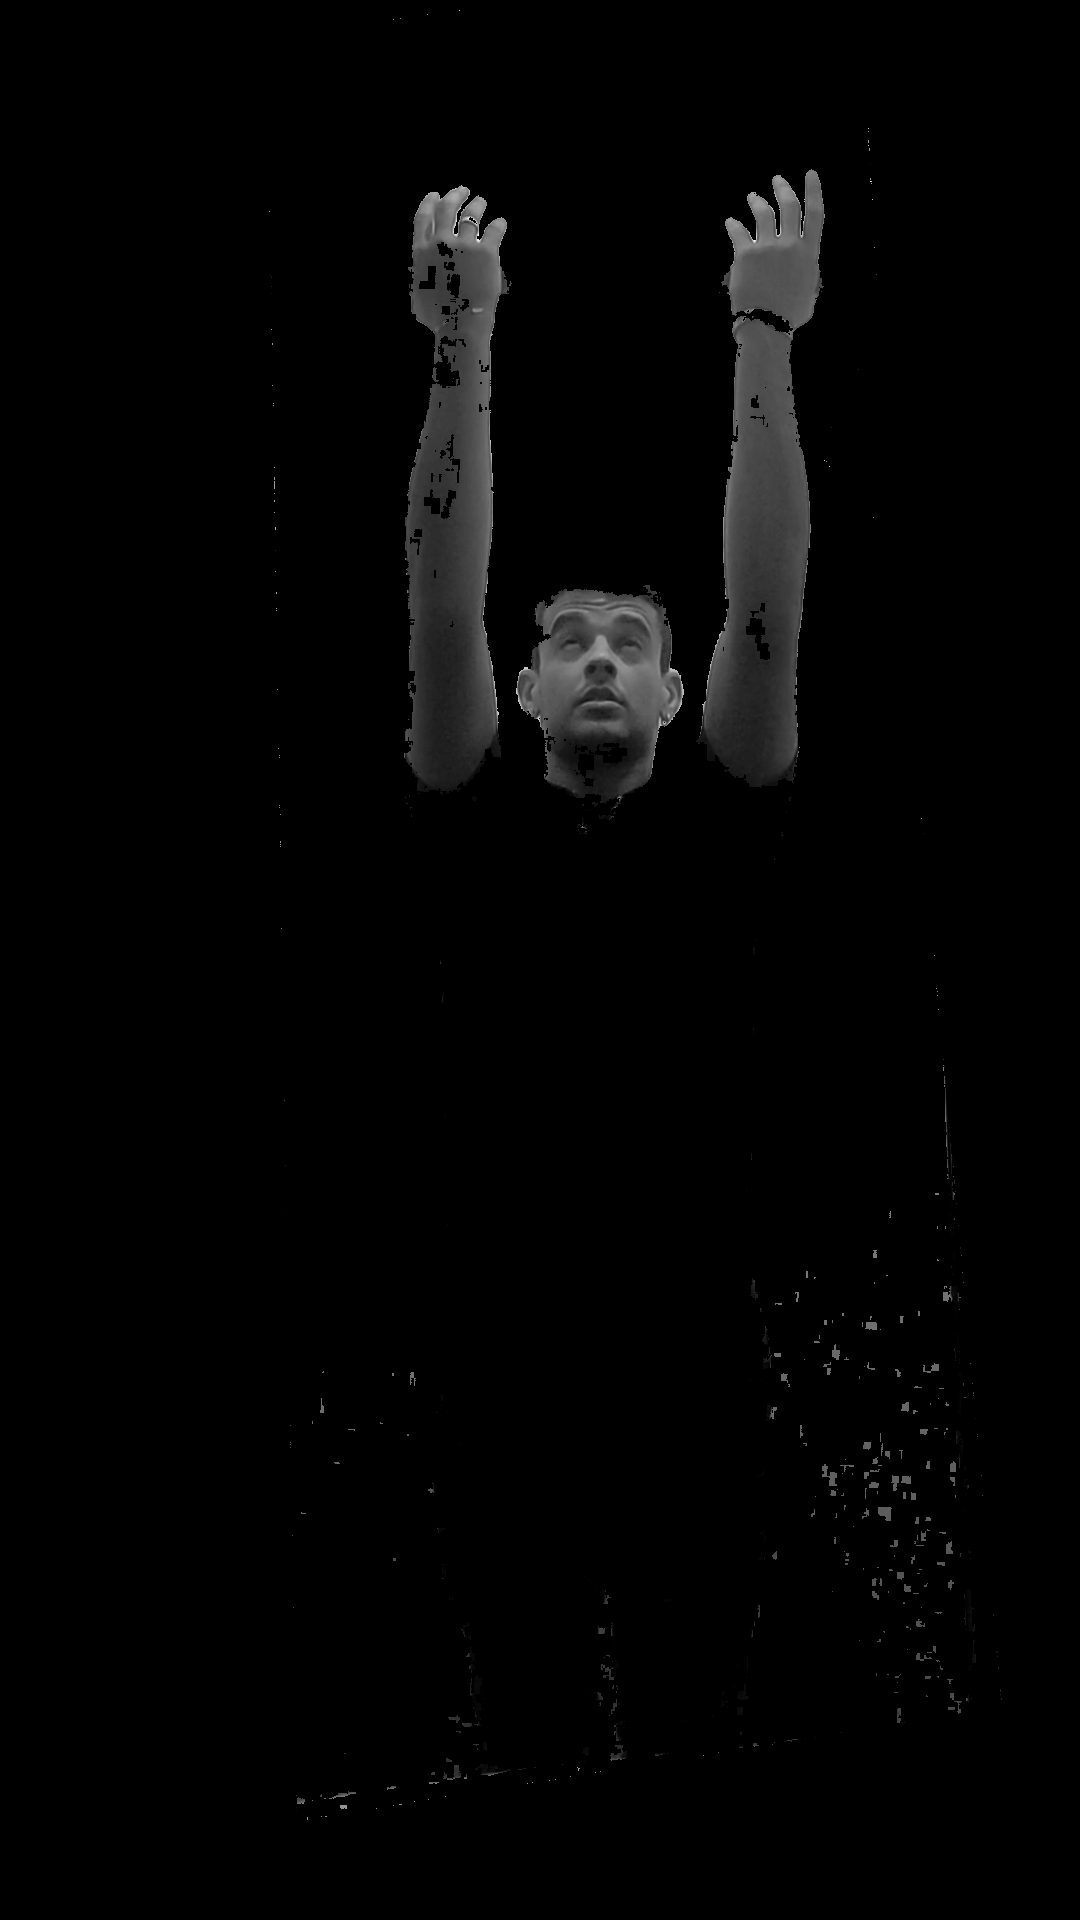
\includegraphics[width=\textwidth]{figuras/mao_barra/gray.png}
        \end{minipage}
        \begin{minipage}{\sizeImg\textwidth}
            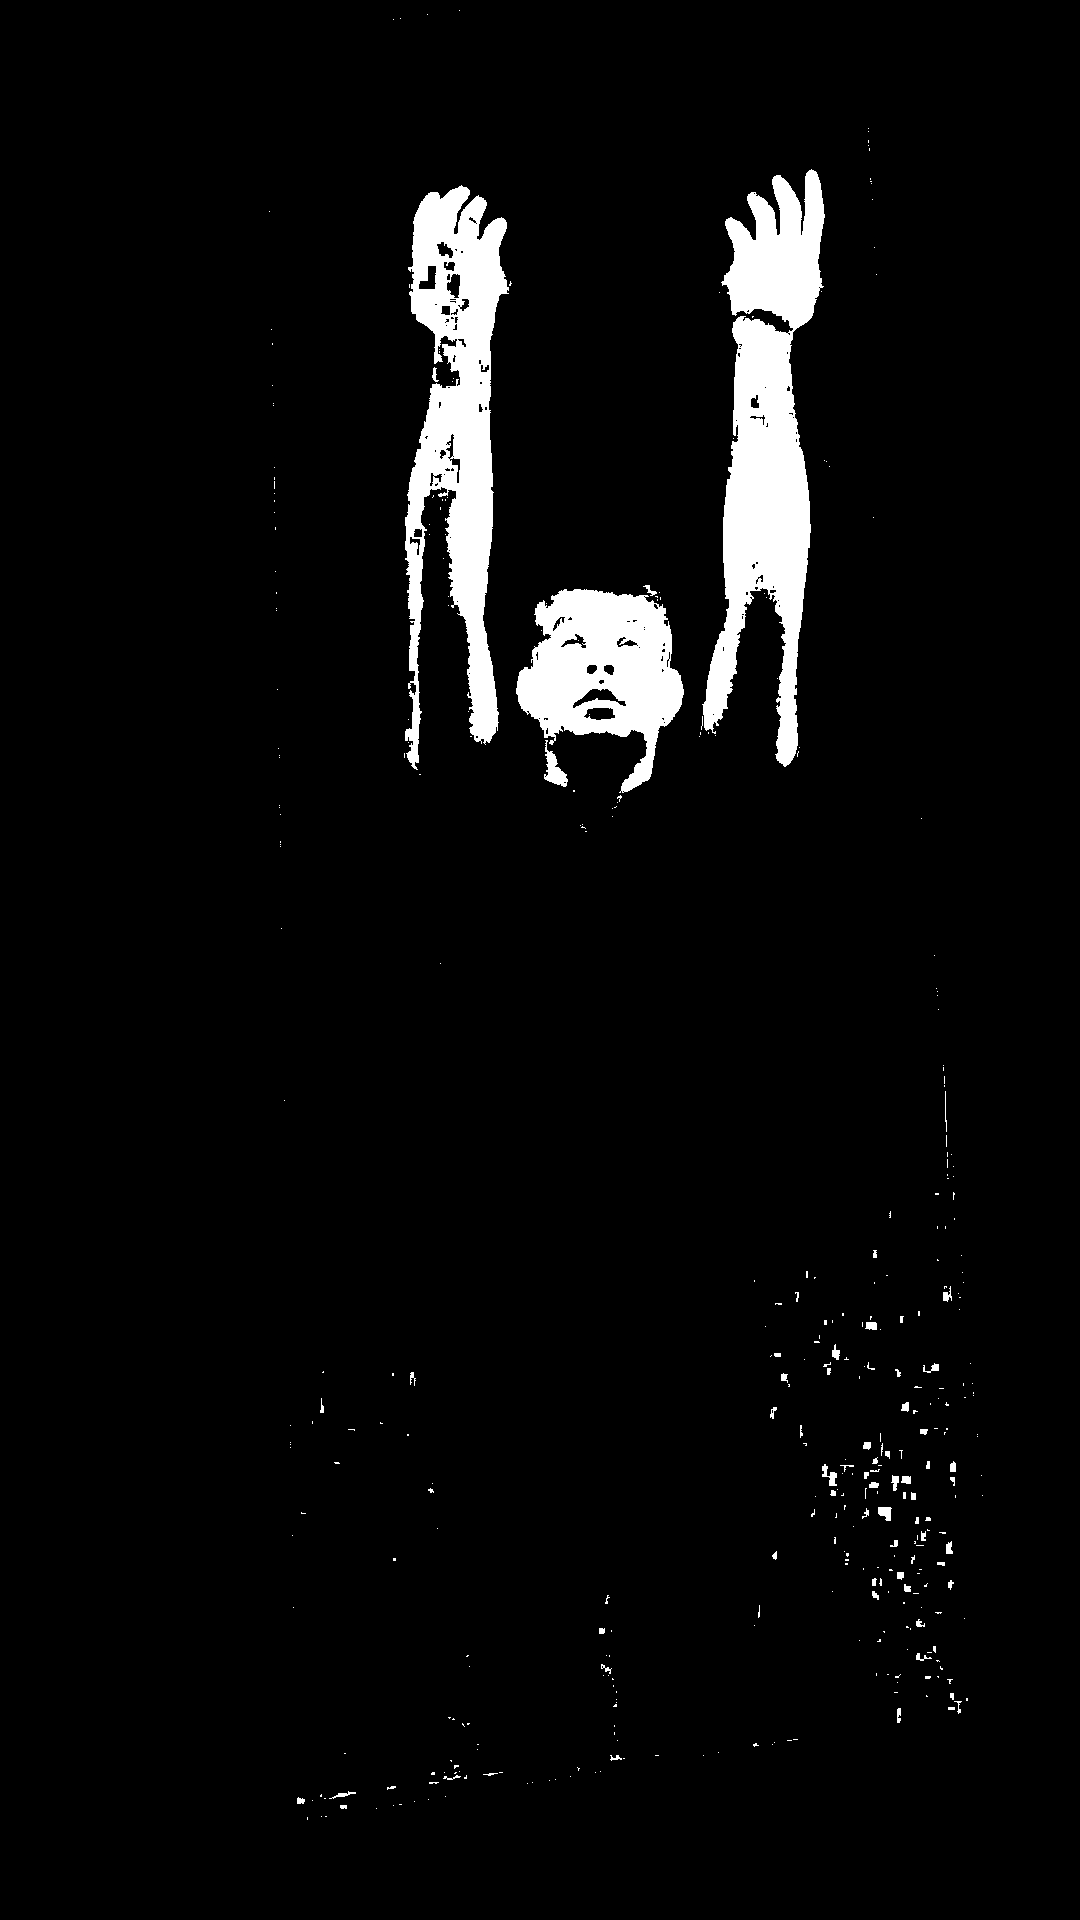
\includegraphics[width=\textwidth]{figuras/mao_barra/limited.png}
        \end{minipage}
    \legend{Fonte: Elaborado pelo autor (2023)}
    \label{fig:gray_limited}
\end{figure}


Com a imagem binarizada, foi aplicado um filtro de suavização usando um kernel quadrado com lados iguais à metade do tamanho da barra. O objetivo dessa etapa é reduzir o ruído na imagem. No entanto, como o filtro de suavização é uma operação de convolução, foi necessário aplicar a limiarização novamente para obter uma nova imagem binarizada.

\begin{figure}[H]
    \centering
    \caption{Redução de ruidos com a suavização e binarização}
        \begin{minipage}{\sizeImg\textwidth}
            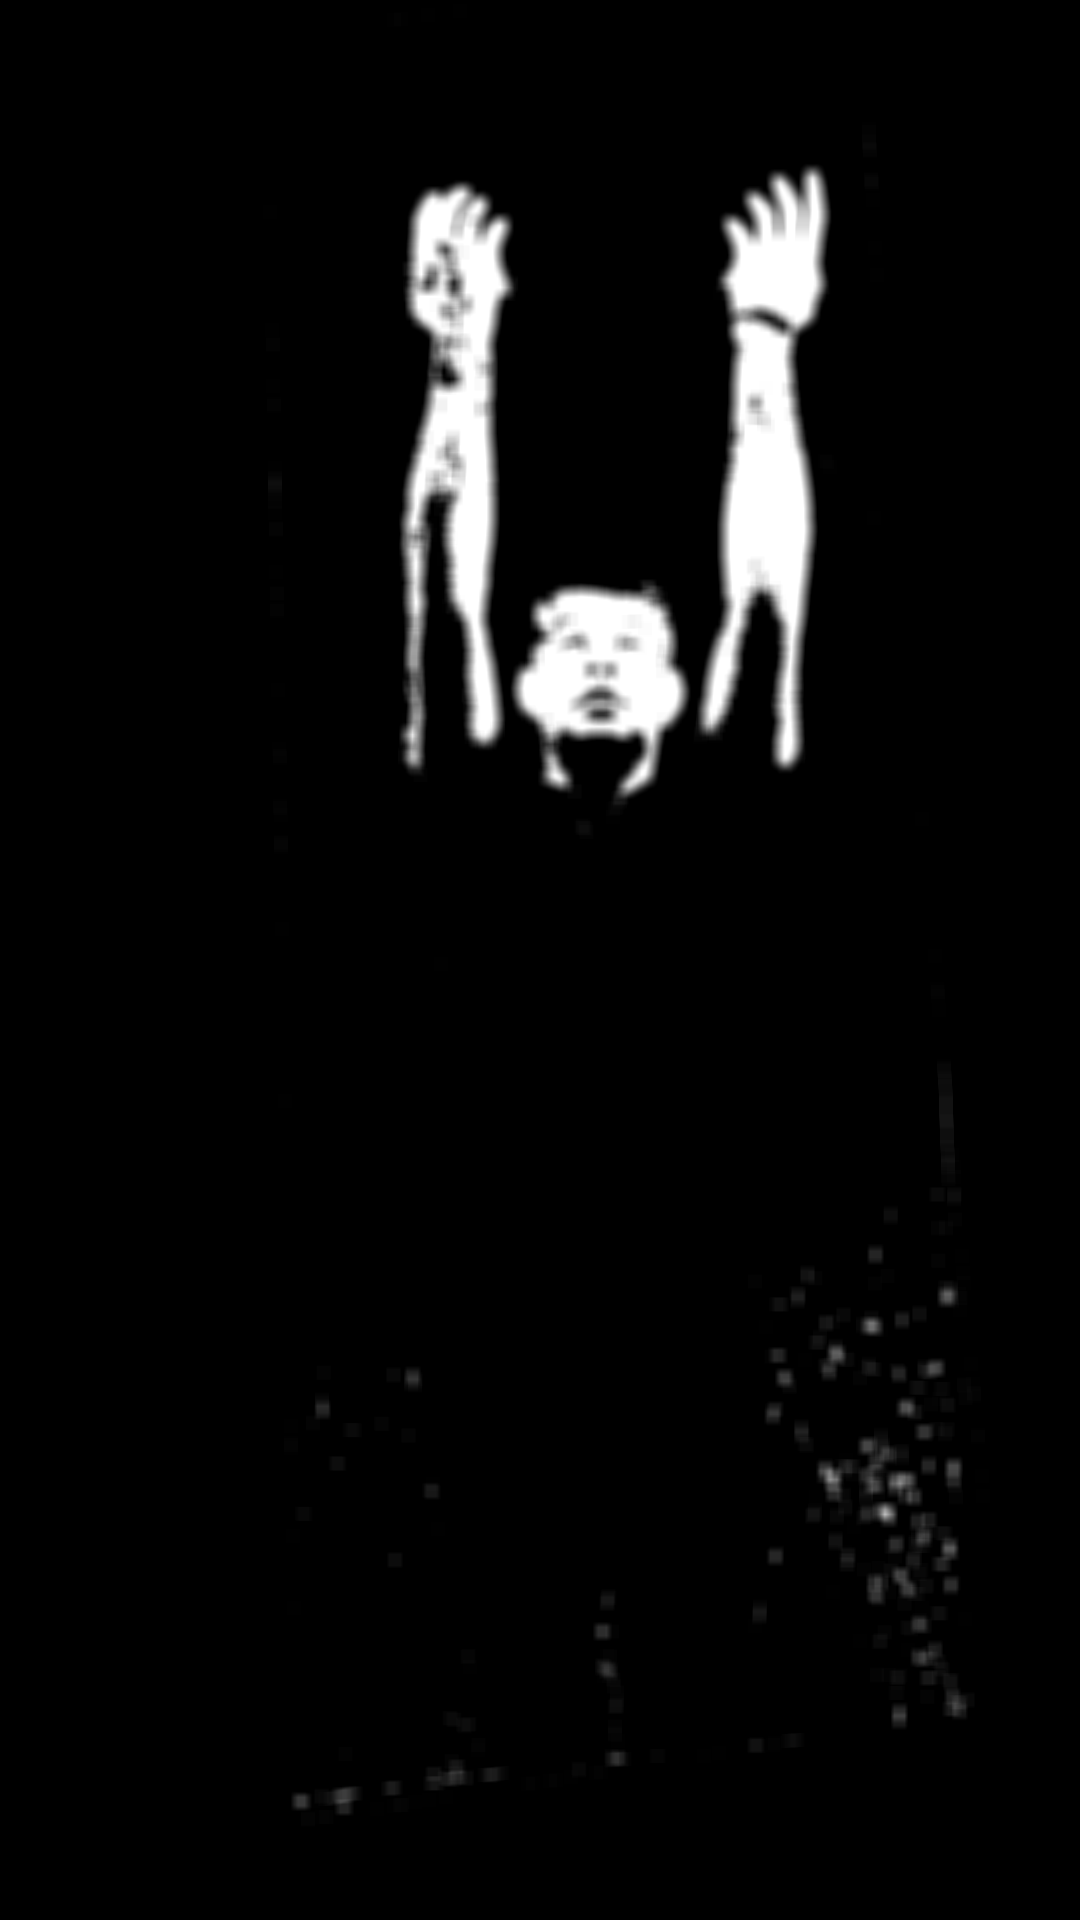
\includegraphics[width=\textwidth]{figuras/mao_barra/blur.png}
        \end{minipage}
        \begin{minipage}{\sizeImg\textwidth}
            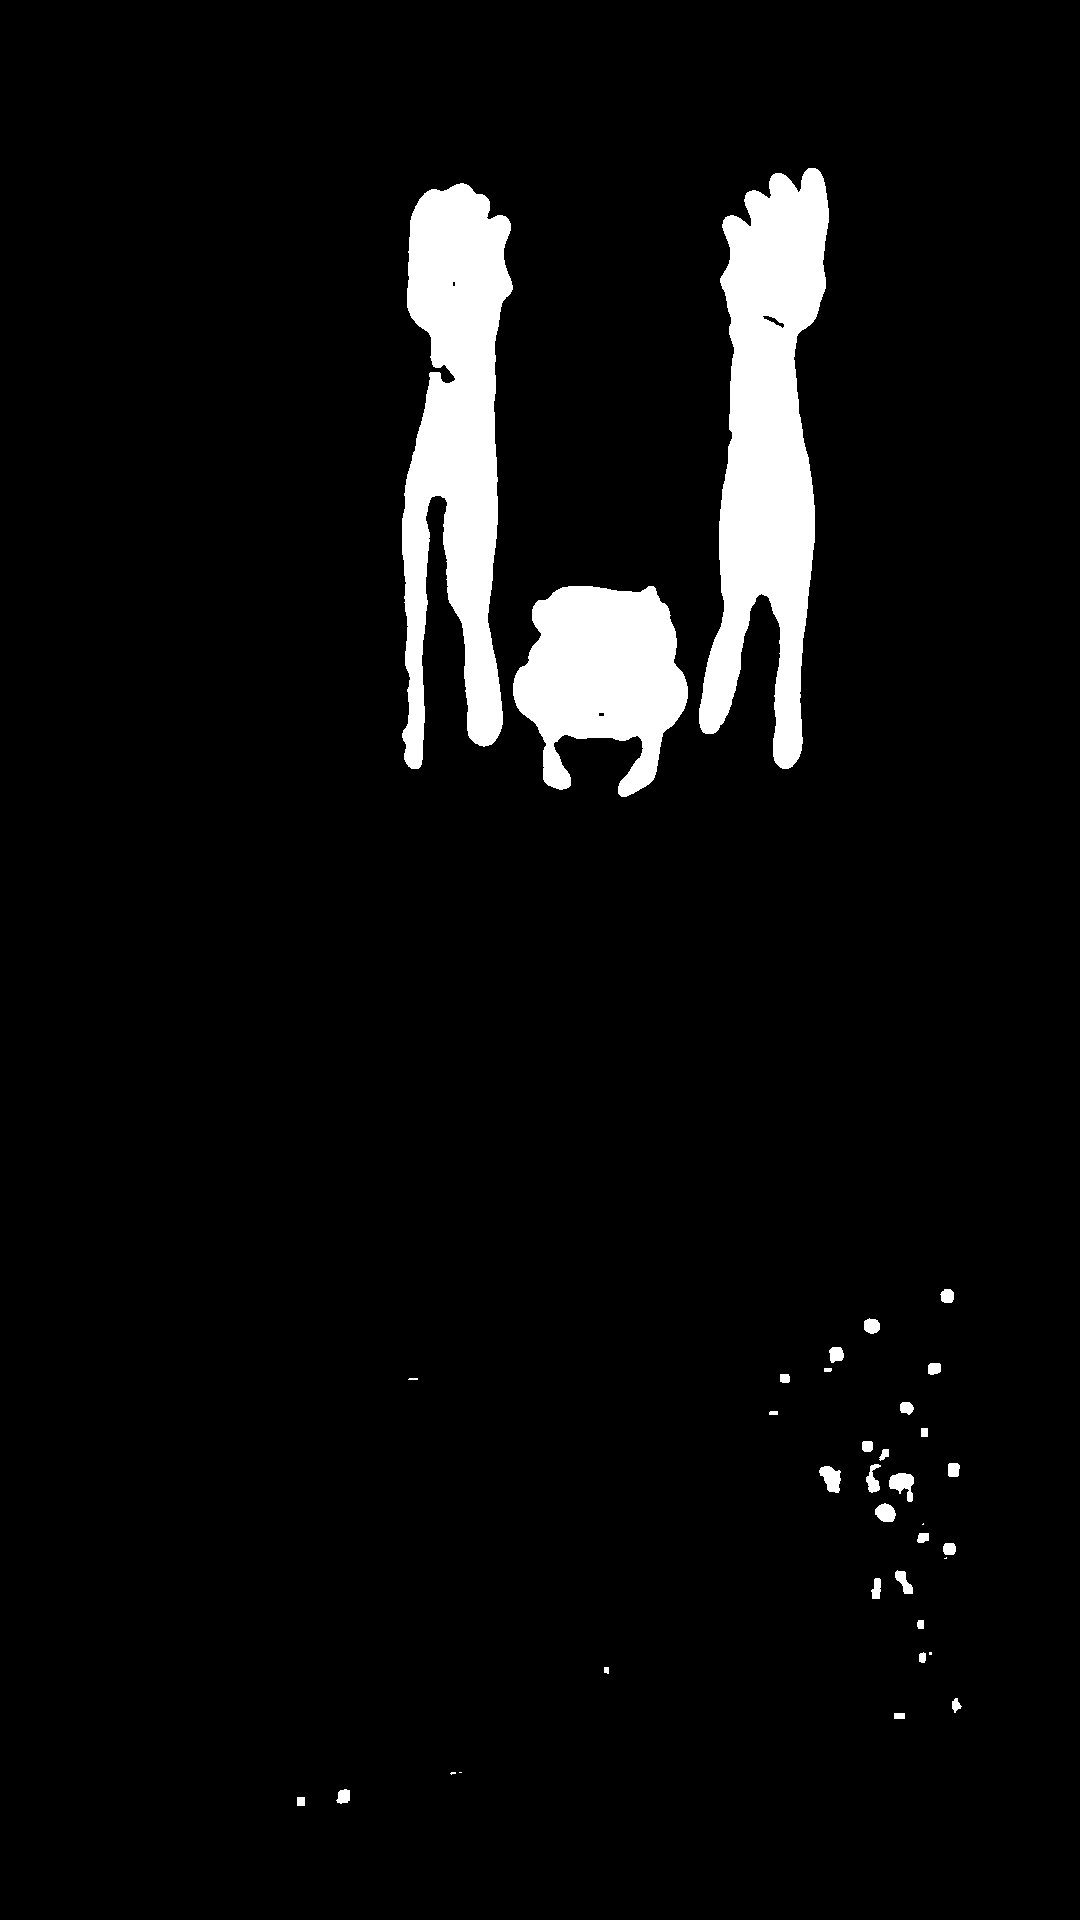
\includegraphics[width=\textwidth]{figuras/mao_barra/limited2.png}
        \end{minipage}
    \legend{Fonte: Elaborado pelo autor (2023)}
    \label{fig:blur}
\end{figure}


Neste ponto, a imagem, que passou por uma segunda binarização para melhorar a precisão e eliminar ruídos de descontinuidade, foi submetida a um filtro de pixelização com um kernel quadrado de lado igual ao tamanho da barra. Esse filtro foi utilizado para destacar claramente a forma do corpo do executor, representando a presença do corpo por blocos de tamanho fixo. Após a pixelização, a limiarização foi aplicada novamente, resultando em uma nova imagem binarizada.

\begin{figure}[H]
    \centering
    \caption{Imagem Pixelizada e binarizada}
        \begin{minipage}{\sizeImg\textwidth}
            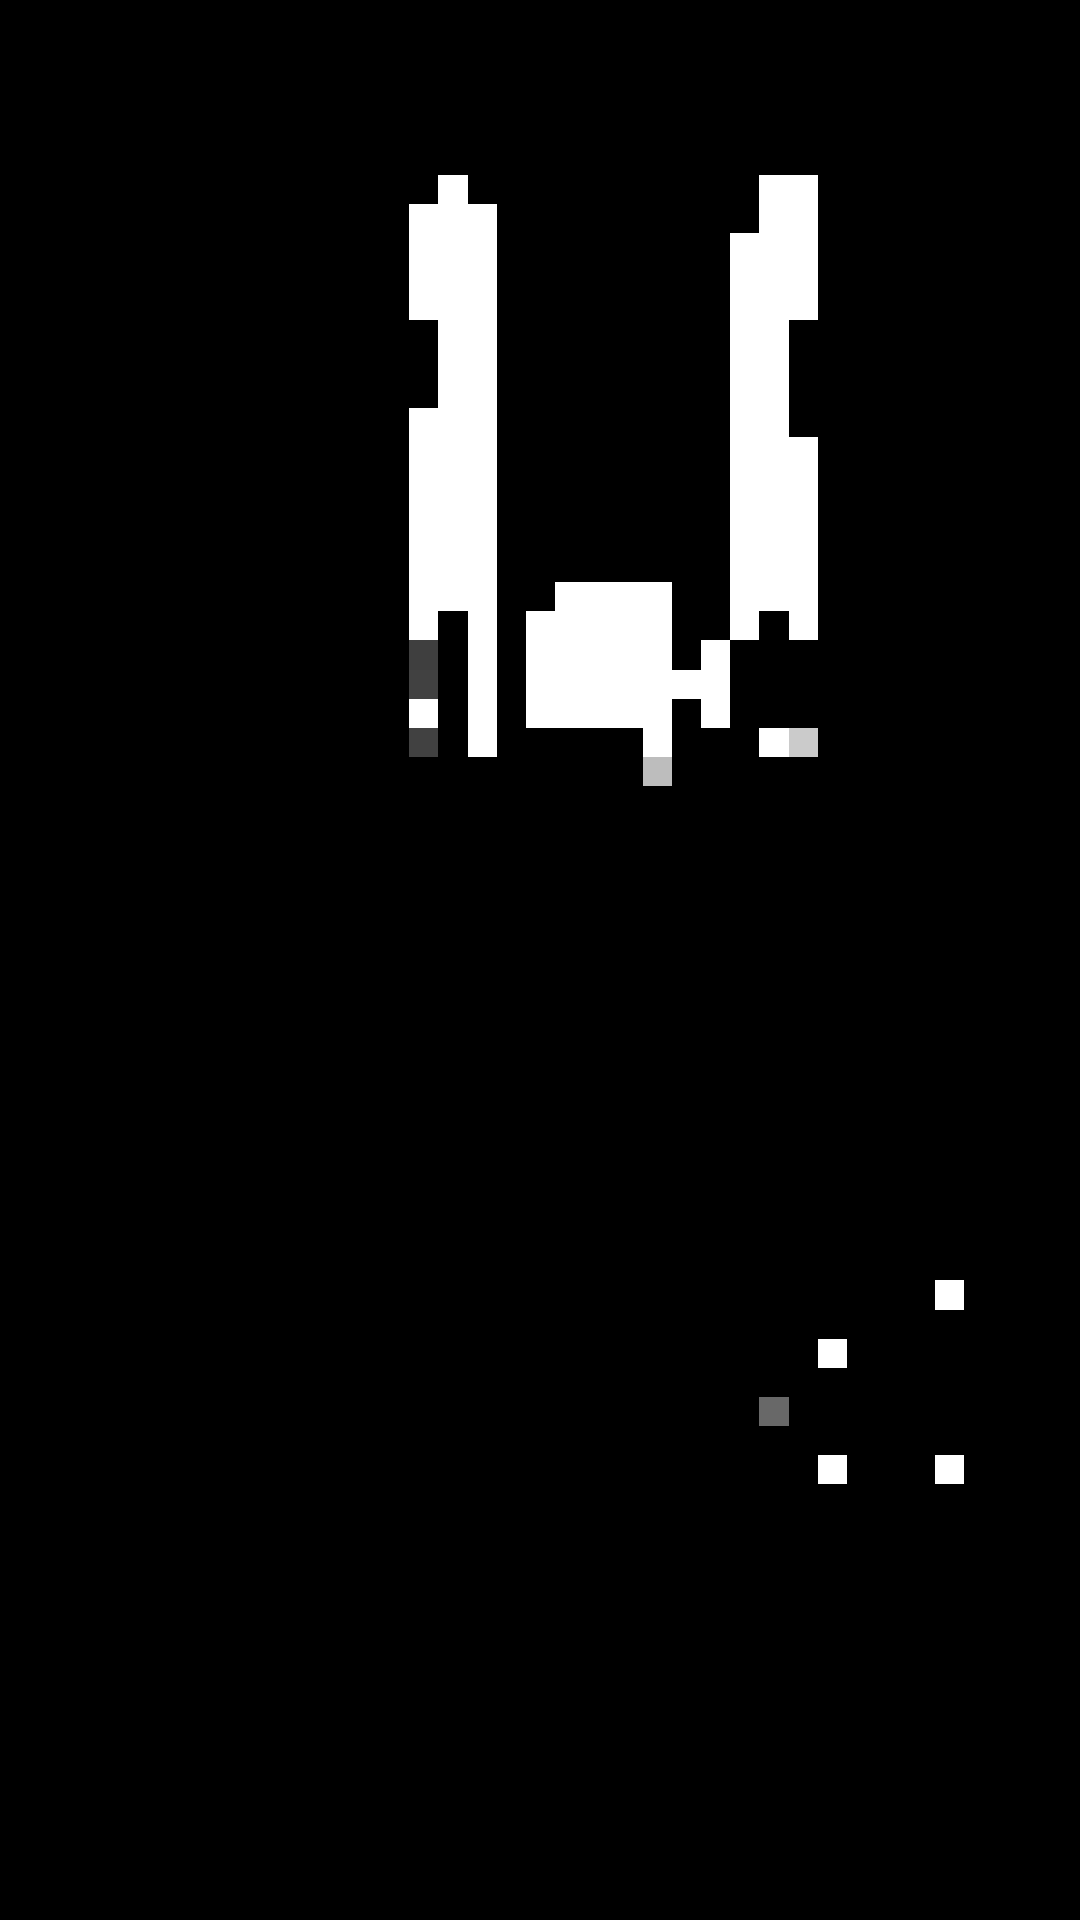
\includegraphics[width=\textwidth]{figuras/mao_barra/pixel.png}
        \end{minipage}
        \begin{minipage}{\sizeImg\textwidth}
            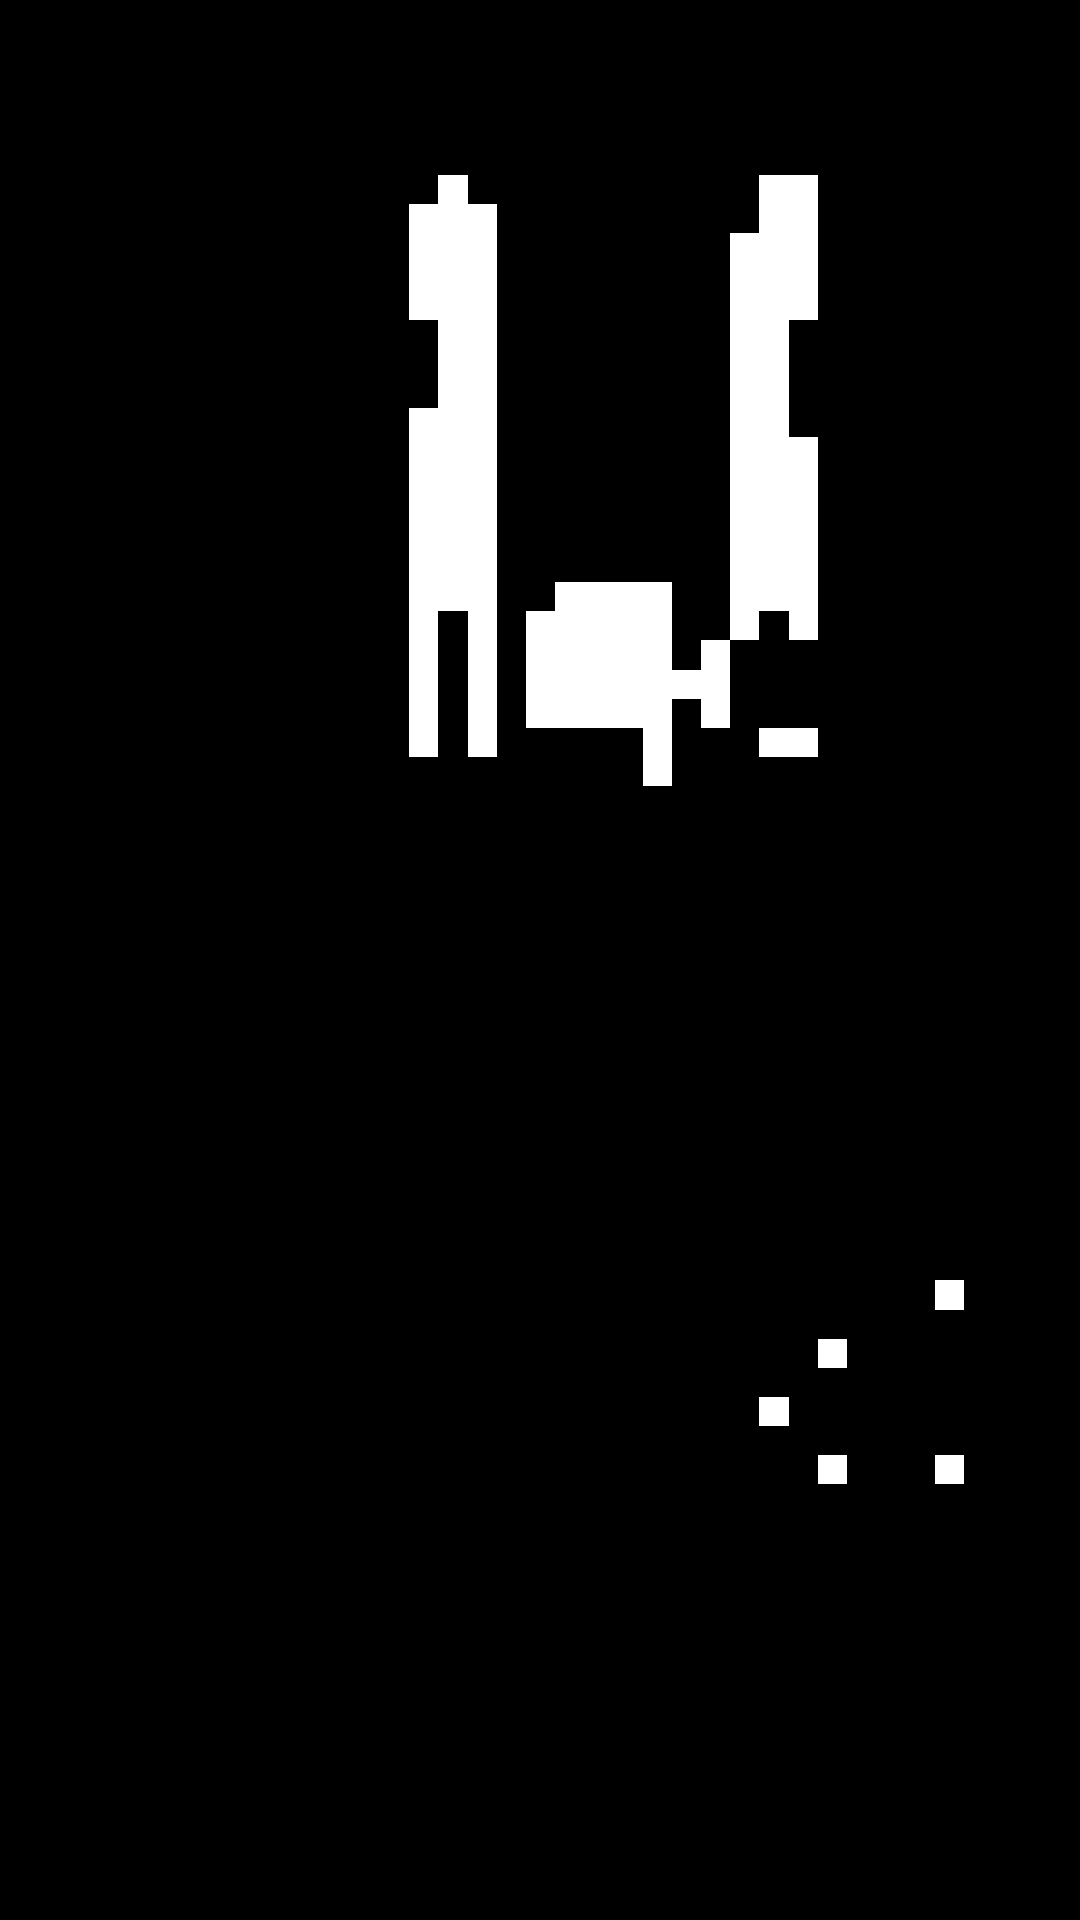
\includegraphics[width=\textwidth]{figuras/mao_barra/limited3.png}
        \end{minipage}
    \legend{Fonte: Elaborado pelo autor (2023)}
    \label{fig:pixeled}
\end{figure}


A área de interesse é representada por uma linha na direção da barra mesclada com uma máscara que divide a barra em dois polos, esquerdo e direito. A divisão desses polos foi feita por meio da identificação do ponto médio entre os ombros esquerdo e direito em relação ao eixo $x$. Com base nesse ponto, foi traçada uma linha vertical paralela à barra, dividindo a imagem em dois polos e forçando uma descontinuidade na região de interesse.

\begin{figure}[H]
    \centering
    \caption{Mascara da região de interesse}
        \begin{minipage}{\sizeImg\textwidth}
            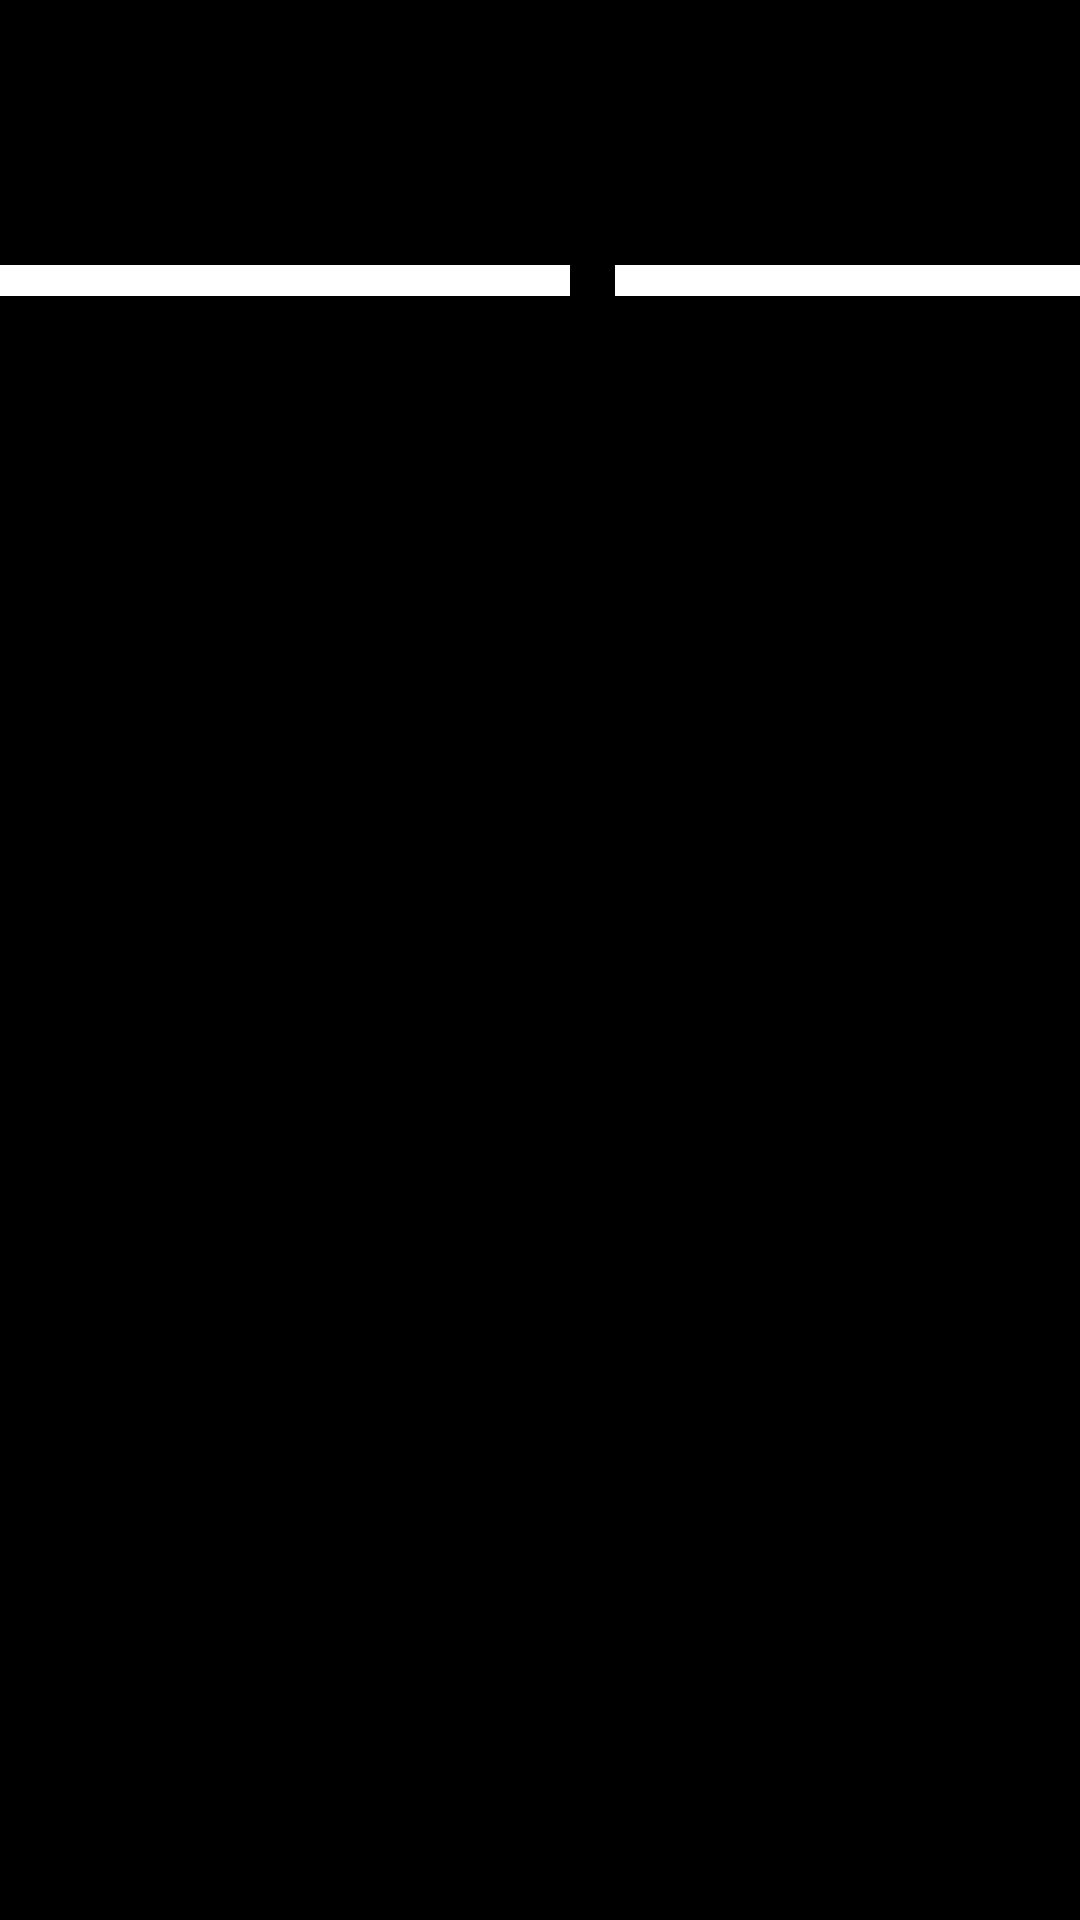
\includegraphics[width=\textwidth]{figuras/mao_barra/mask3.png}
        \end{minipage}
    \legend{Fonte: Elaborado pelo autor (2023)}
    \label{fig:mask}
\end{figure}


Por fim, com a imagem filtrada e binarizada, foi destacada a região de interesse e identificados os contornos presentes nessa região. Cada contorno representa algo obstruindo a barra, especificamente uma parte do corpo ou algo que tenha o mesmo intervalo de cor previamente estabelecido. Portanto, com a identificação de 1 ou mais contornos em cada lado da imagem, possivelmente são as mãos tocando a barra.

\begin{figure}[H]
    \centering
    \caption{Do lado esquerdo a imagem segmentada e do lado direto sua representação}
        \begin{minipage}{\sizeImg\textwidth}
            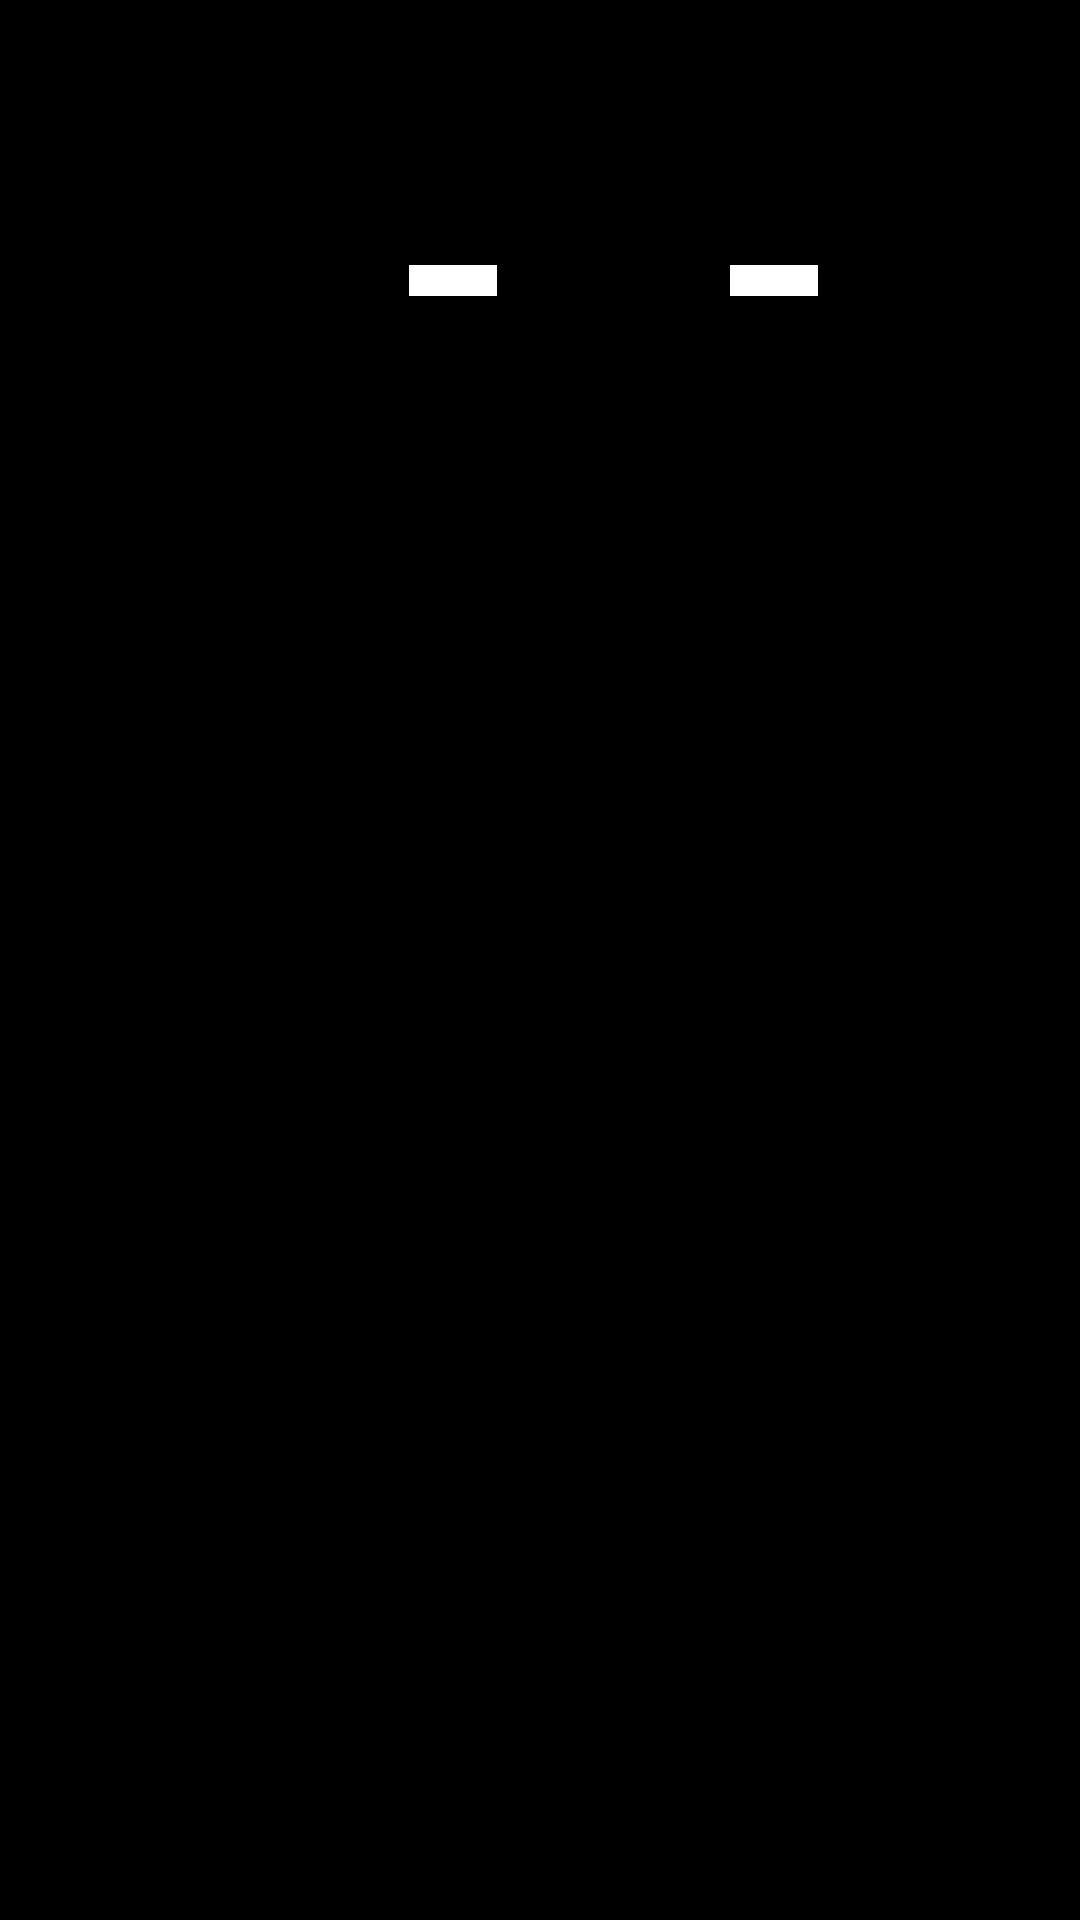
\includegraphics[width=\textwidth]{figuras/mao_barra/only_hands.png}
        \end{minipage}
        \begin{minipage}{\sizeImg\textwidth}
            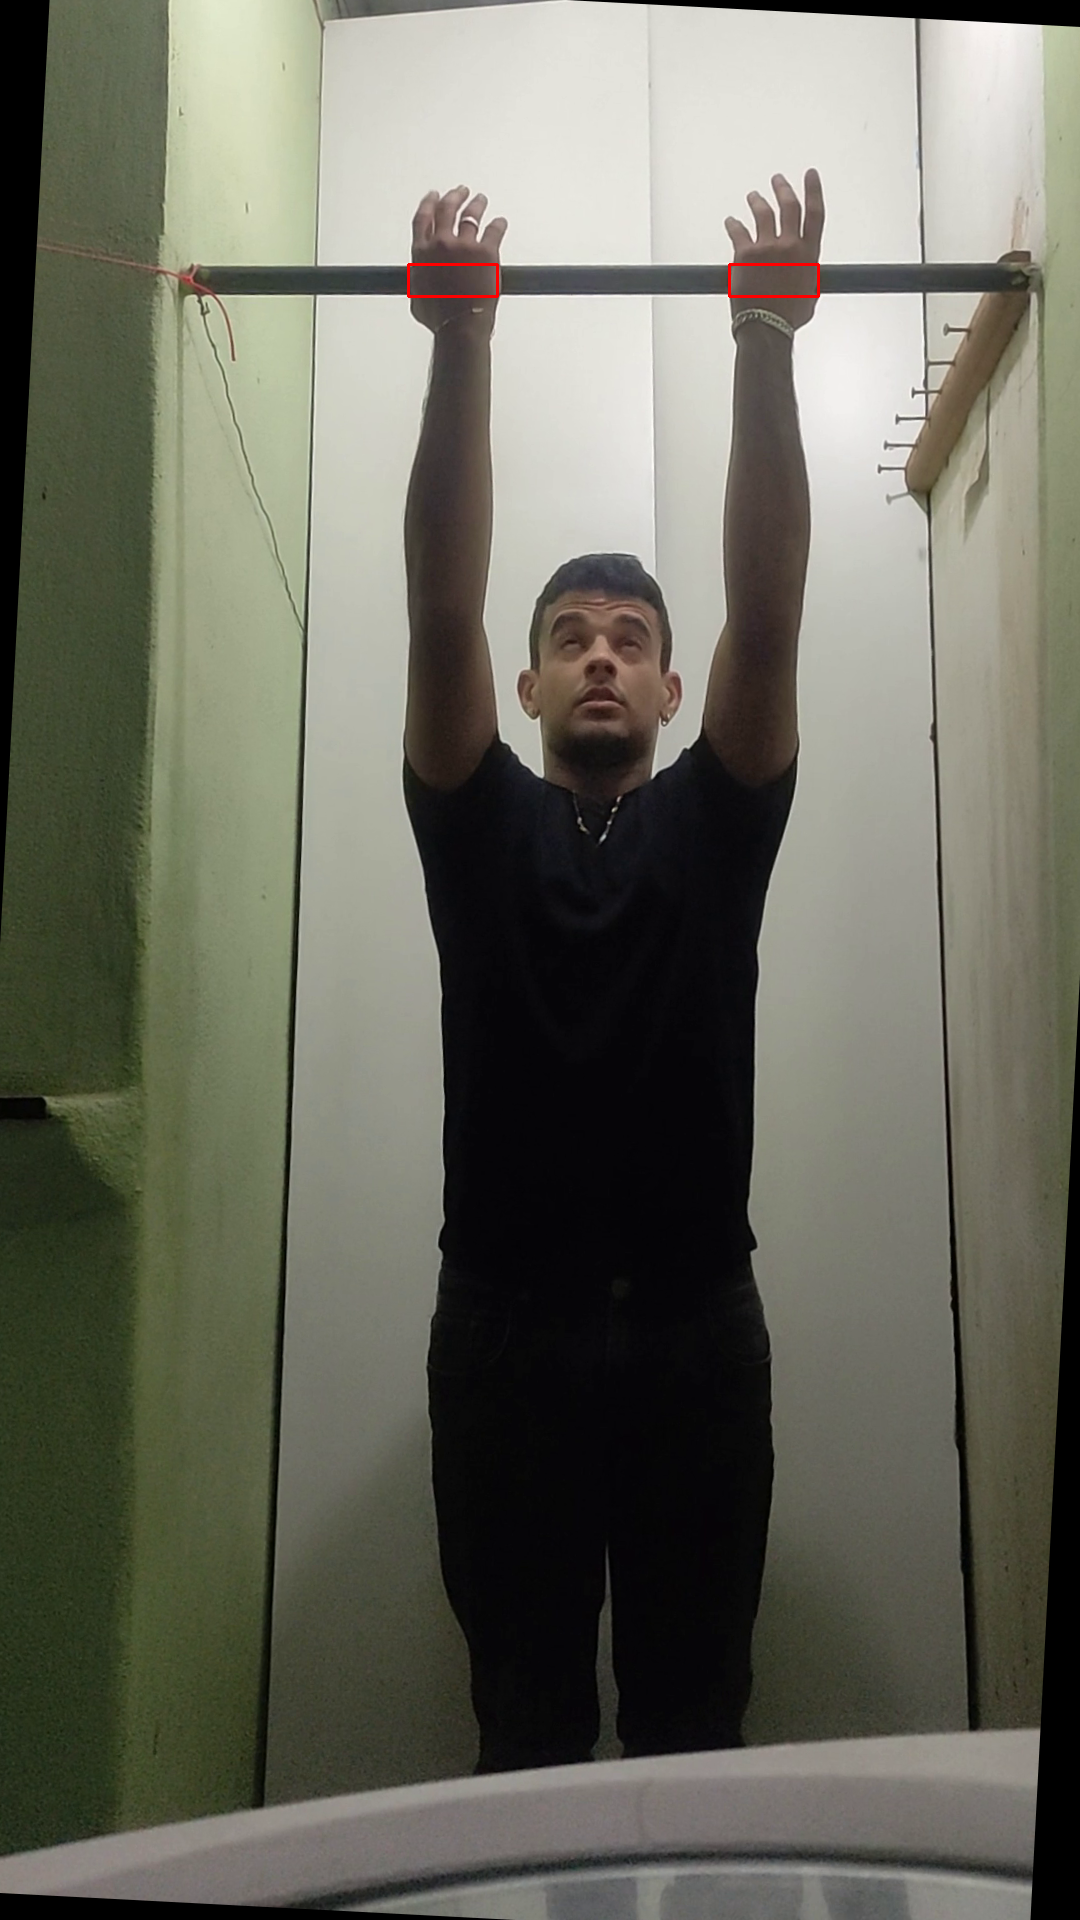
\includegraphics[width=\textwidth]{figuras/mao_barra/contornos.png}
        \end{minipage}
    \legend{Fonte: Elaborado pelo autor (2023)}
    \label{fig:binHand}
\end{figure}




O processo pode ser visualizado no diagrama a seguir:
\begin{figure}[H]
	\centering
    \caption{Diagrama do processo de detecção de mão na barra}
	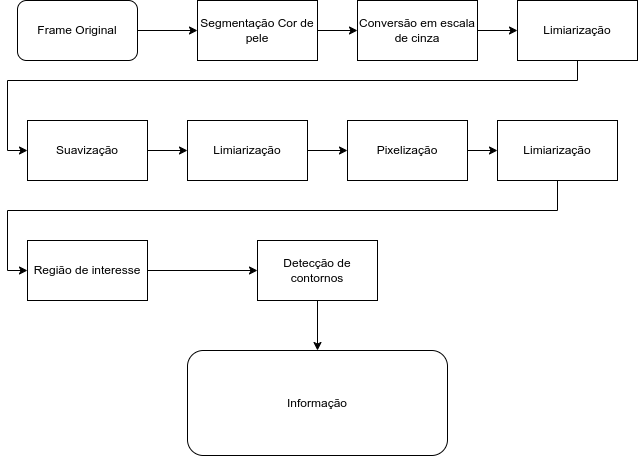
\includegraphics[scale=0.7]{figuras/diagrama/mao_barra.png}
    \legend{Fonte: Elaborado pelo autor (2023)}
	\label{dia:mao_barra}
\end{figure}

\subsection[Braço esticado]{Braço esticado}\label{sec:Braco esticado}

A verificação da extensão do cotovelo foi realizada estritamente quando o executor estava com as mãos na barra de maneira contínua, quadro a quadro, verificando duas condições denominadas aqui como $check\_1$ e $check\_2$. A extensão total do braço só foi considerada quando ambas as condições foram atendidas. Esse processo de verificação ajudou a garantir que somente certas condições fossem identificadas como verdadeiras, reduzindo ao máximo a ocorrência de falsos positivos e melhorando a confiabilidade da verificação da extensão do cotovelo. Isso torna o processo mais robusto em relação a possíveis fontes de erro ou variações nos dados de entrada.


$check\_1$ foi estabelecido com base na comparação dos ângulos formados entre o antebraço e o braço. Nessa avaliação, o antebraço era representado pelo segmento de reta definido pelos pontos do punho e cotovelo, enquanto o braço era representado pelo segmento de reta definido pelos pontos do ombro e cotovelo. Para que a condição $check\_1$ fosse considerada verdadeira, era necessário que tanto o ângulo formado pelo antebraço e braço esquerdo quanto o ângulo formado pelo antebraço e braço direito fossem menores que o limite previamente estabelecido em 13º (valor do limiar).\label{angulo_braco}

\begin{figure}[H]
	\centering
    \caption{Segmento de reta representante dos membros superiores}
	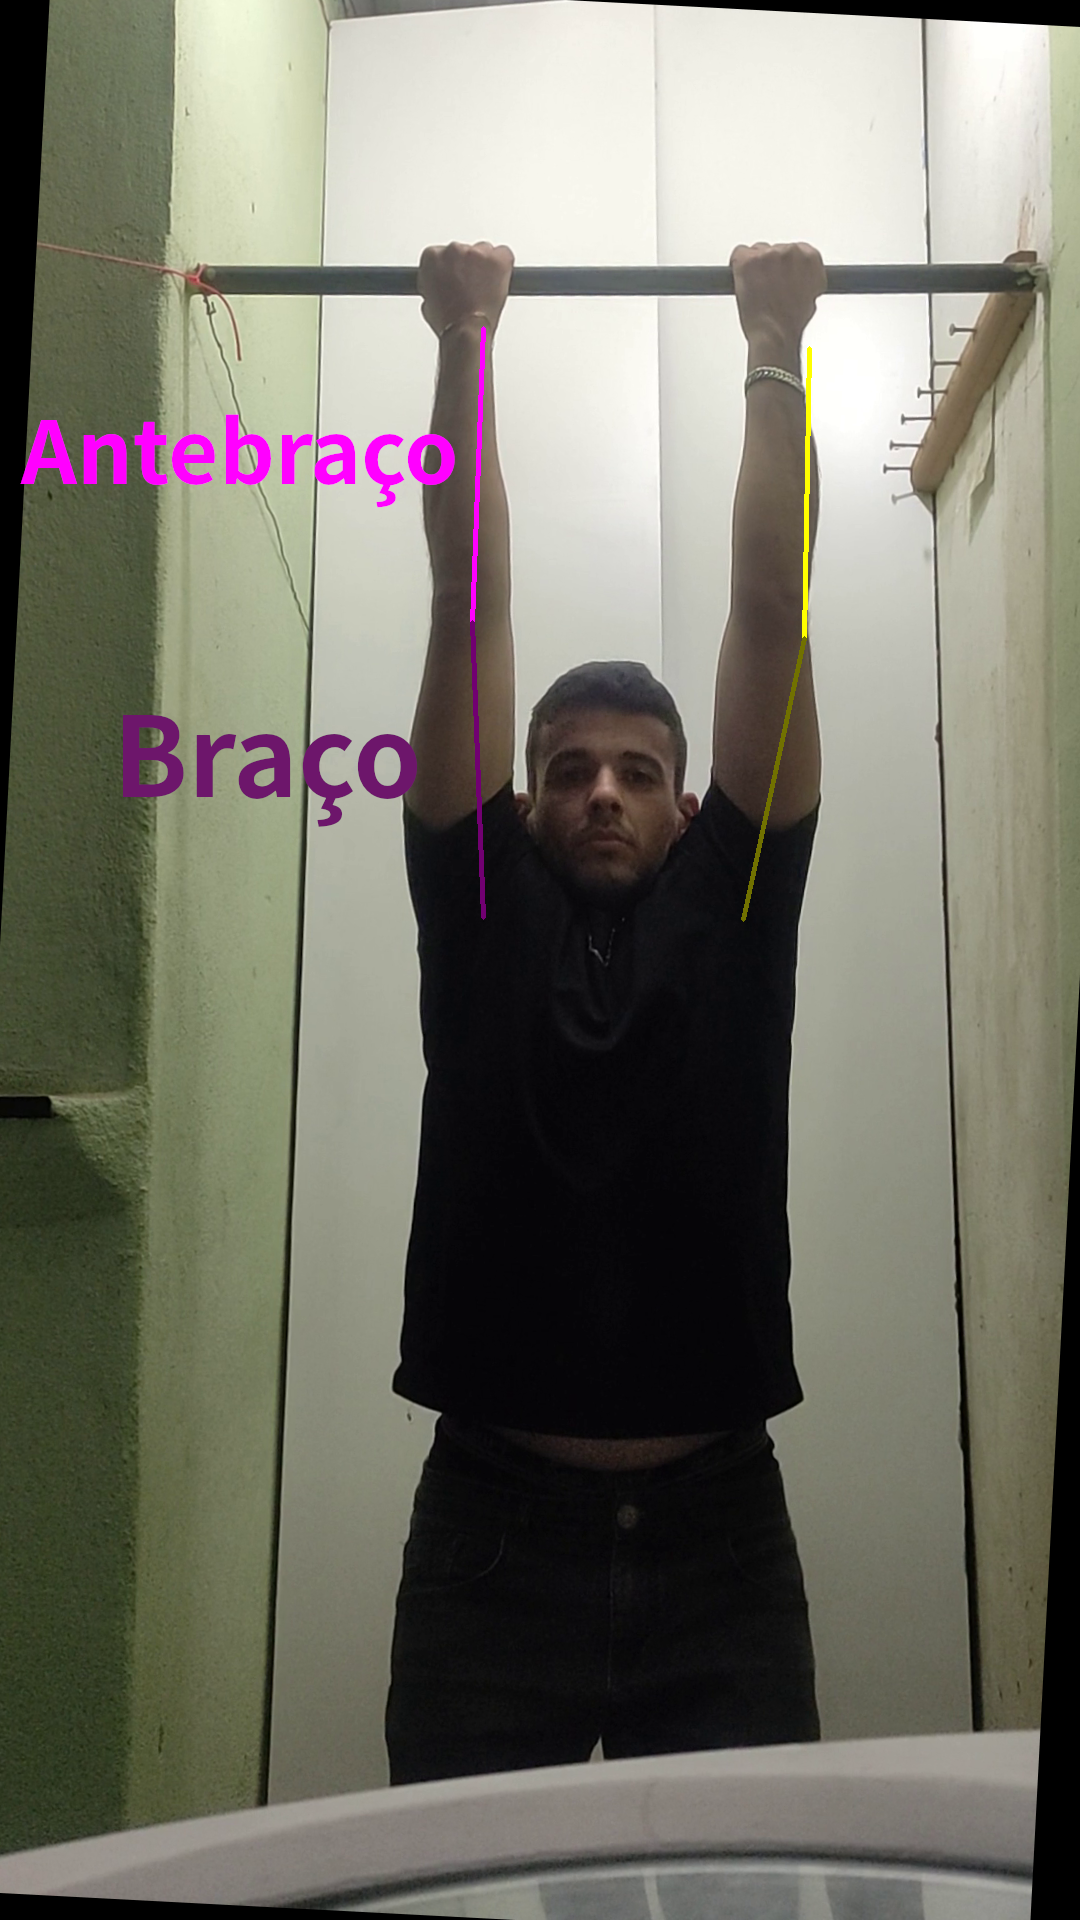
\includegraphics[scale=0.2]{figuras/braco_esticado/82_braco_antebraco.png}
    \legend{Fonte: Elaborado pelo autor (2023)}
	\label{fig:braco_antebraco}
\end{figure}

$check\_2$ foi estabelecido com base na medição da distância entre o peito do executor e a barra. Devido à rotação prévia do frame em relação à barra e à garantia de que a barra é paralela ao solo, a medida utilizou exclusivamente a coordenada $y$.

Foi utilizado uma variável como parâmetro, sendo atualizada frame a frame ao longo do vídeo. Essa variável registra a posição do peito no momento em que a maior distância entre o peito e a barra é identificada.

Em termos práticos, $check\_2$ avaliava se a diferença absoluta entre o ombro esquerdo e o valor armazenado do ombro esquerdo, quando identificada a maior distância entre peito e a barra, era menor que o limite predefinido de 100 pixels. O mesmo critério era aplicado tanto ao ombro direito quanto ao ombro esquerdo.

Quando essa condição era atendida em um dos lados, a verificação era considerada verdadeira. A verificação unilateral era suficiente devido à imprecisão na determinação exata da posição do ombro, que poderia estar dentro do intervalo aceitável em um lado e fora do intervalo no outro por um valor ínfimo de 1 pixel.

Ao exigir que ambas as mãos estivessem tocando a barra, o alinhamento do peito tendia a ocorrer de forma paralela à barra. Isso implicava que, ao considerar um lado como verdadeiro, o outro também é automaticamente considerado verdadeiro, salvo em casos onde um cotovelo está estendido e o outro está flexionado. No entanto, esses casos são cobertos pelo $check\_1$, onde é verificada a angulação dos dois cotovelos, tanto esquerdo quanto direito.


\begin{figure}[H]
	\centering
    \caption{Diagrama do fluxo da informação para verificar extensão do cotovelo}
	\includegraphics[scale=0.7]{figuras/diagrama/extensão.png}
    \legend{Fonte: Elaborado pelo autor (2023)}
	\label{dia:extensao}
\end{figure}





\subsection[Ultrapassagem do queixo a barra]{Ultrapassagem do queixo a barra}\label{sec:meta}

Para verificar se ocorreu a ultrapassagem do queixo à barra, foram avaliadas três condições essenciais: a posição do peito em relação à barra, a flexão do cotovelo e a detecção de uma presença na área de interesse, presumivelmente correspondente à cabeça do executor. As condições são verificadas na ordem apresentada, e para evitar processamento desnecessário, as condições são analisadas apenas se a mão estiver encostando na barra. A cada condição falsa, o processamento é interrompido.

\begin{figure}[H]
	\centering
    \caption{Diagrama Ultrapassagem do queixo a barra }
	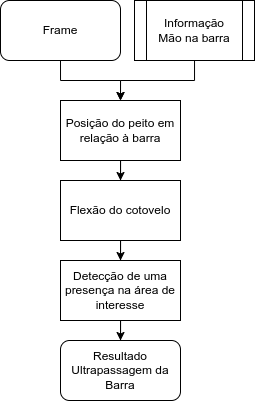
\includegraphics[scale=0.75]{figuras/diagrama/ultrapassagem_barra.png}
    \legend{Fonte: Elaborado pelo autor (2023)}
	\label{dia:ultrapassagem}
\end{figure}


A verificação da proximidade do peito em relação à barra é determinada pela medida da distância da coordenada entre os ombros esquerdo ou direito até a barra, com foco na coordenada $y$. Considera-se que o peito está em contato com a barra quando a distância entre o peito e a barra é inferior a 150\% do comprimento da própria barra.

Portanto, a ultrapassagem bem-sucedida do queixo à barra é confirmada apenas quando todas as três condições - a proximidade do peito à barra, a flexão do cotovelo e a detecção de elementos na região de interesse - são avaliadas como verdadeiras.

O processamento para verificar a flexão de cotovelo segue uma abordagem semelhante ao processo de verificação de extensão de cotovelo utilizado na detecção de mão na barra. A diferença é que, nesse caso, examinamos se o ângulo formado entre os segmentos que representam o antebraço e o braço esquerdo ou direito é superior a 175 graus, incorporando uma margem de imprecisão de 5 graus.

Por fim, o processo de detecção de presença na área de interesse segue uma abordagem semelhante àquela utilizada na detecção da mão na barra. Inicialmente, a imagem passa por um processo de realce da cor da pele. Em seguida, é convertida para escala de cinza e, posteriormente, submetida à limiarização, resultando em uma imagem binarizada na qual o executor se destaca em relação ao plano de fundo.

\renewcommand{\sizeImg}{0.2}
\begin{figure}[H]
    \caption{Preprocessamento até a binarização da imagem}
    \centering
        \begin{minipage}{\sizeImg\textwidth}
            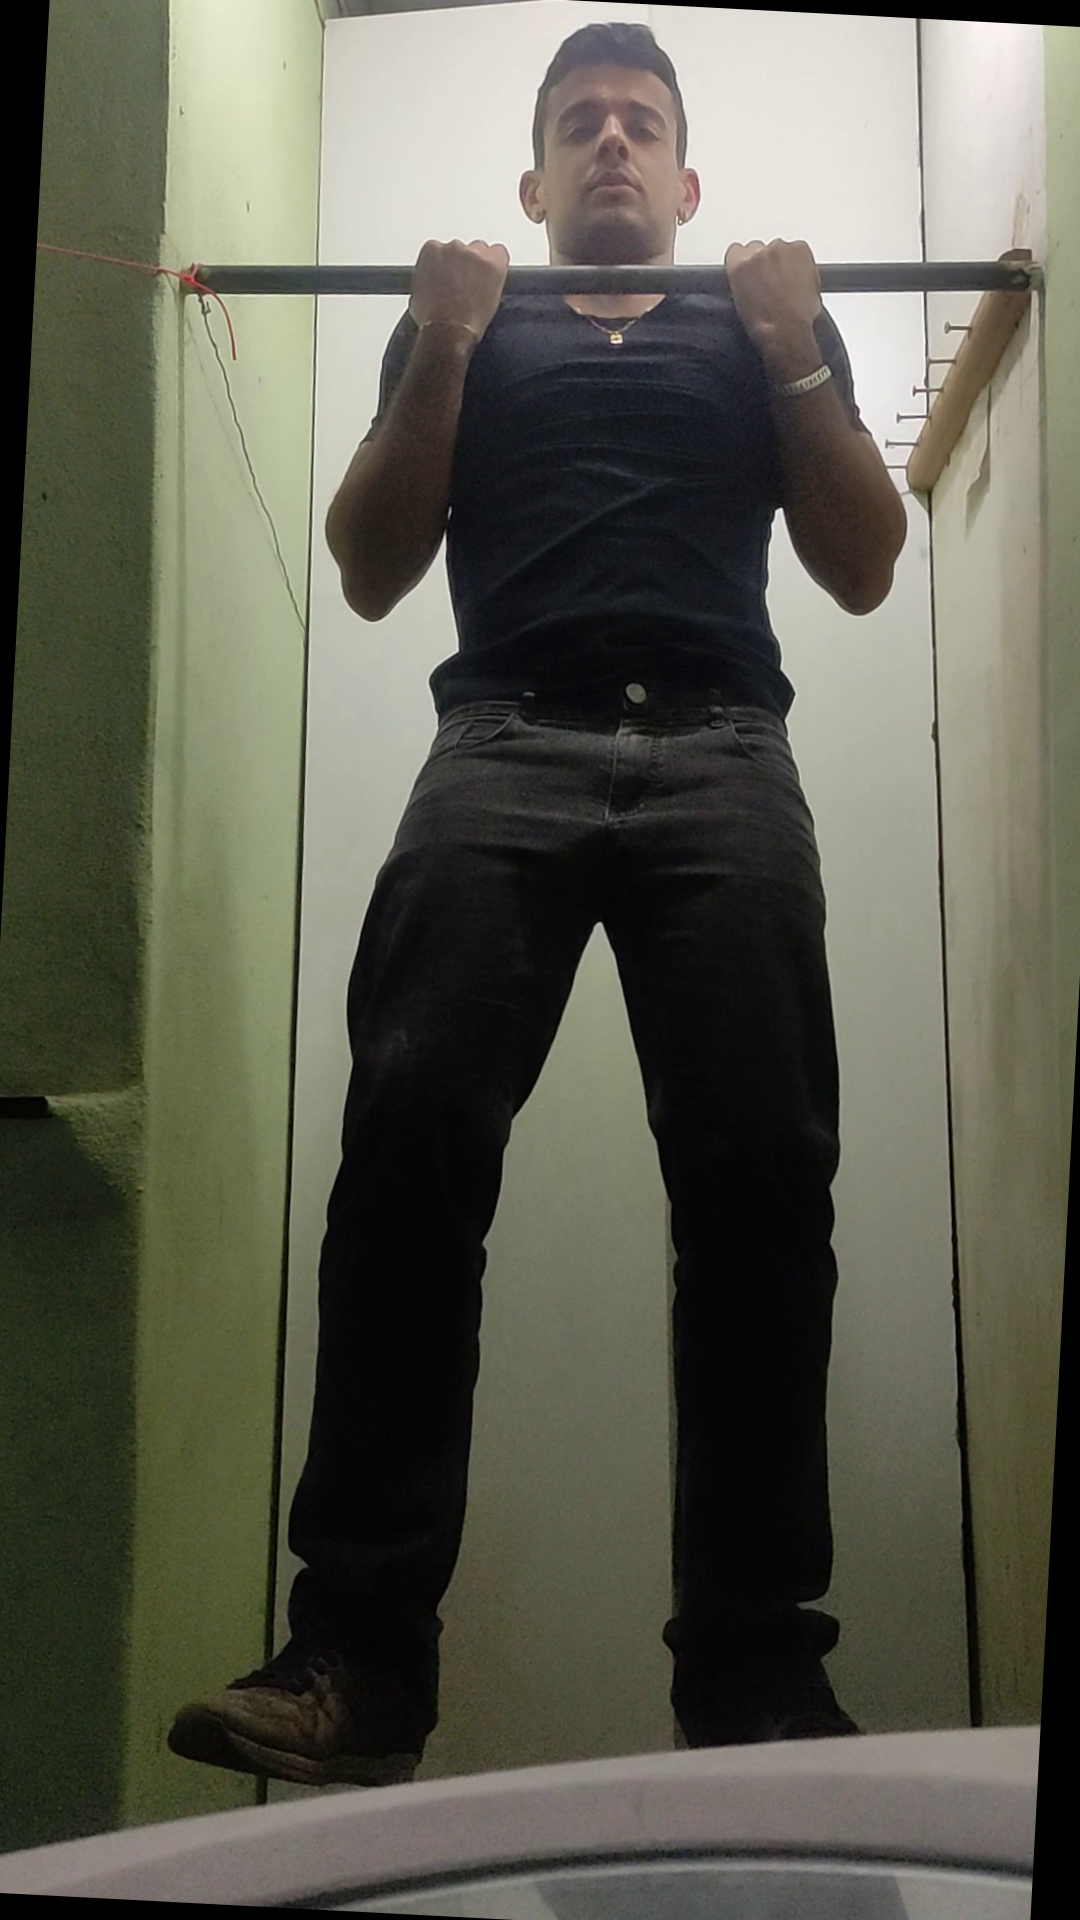
\includegraphics[width=\textwidth]{figuras/ultrapassar_barra/134_original.png}
        \end{minipage}
        \begin{minipage}{\sizeImg\textwidth}
            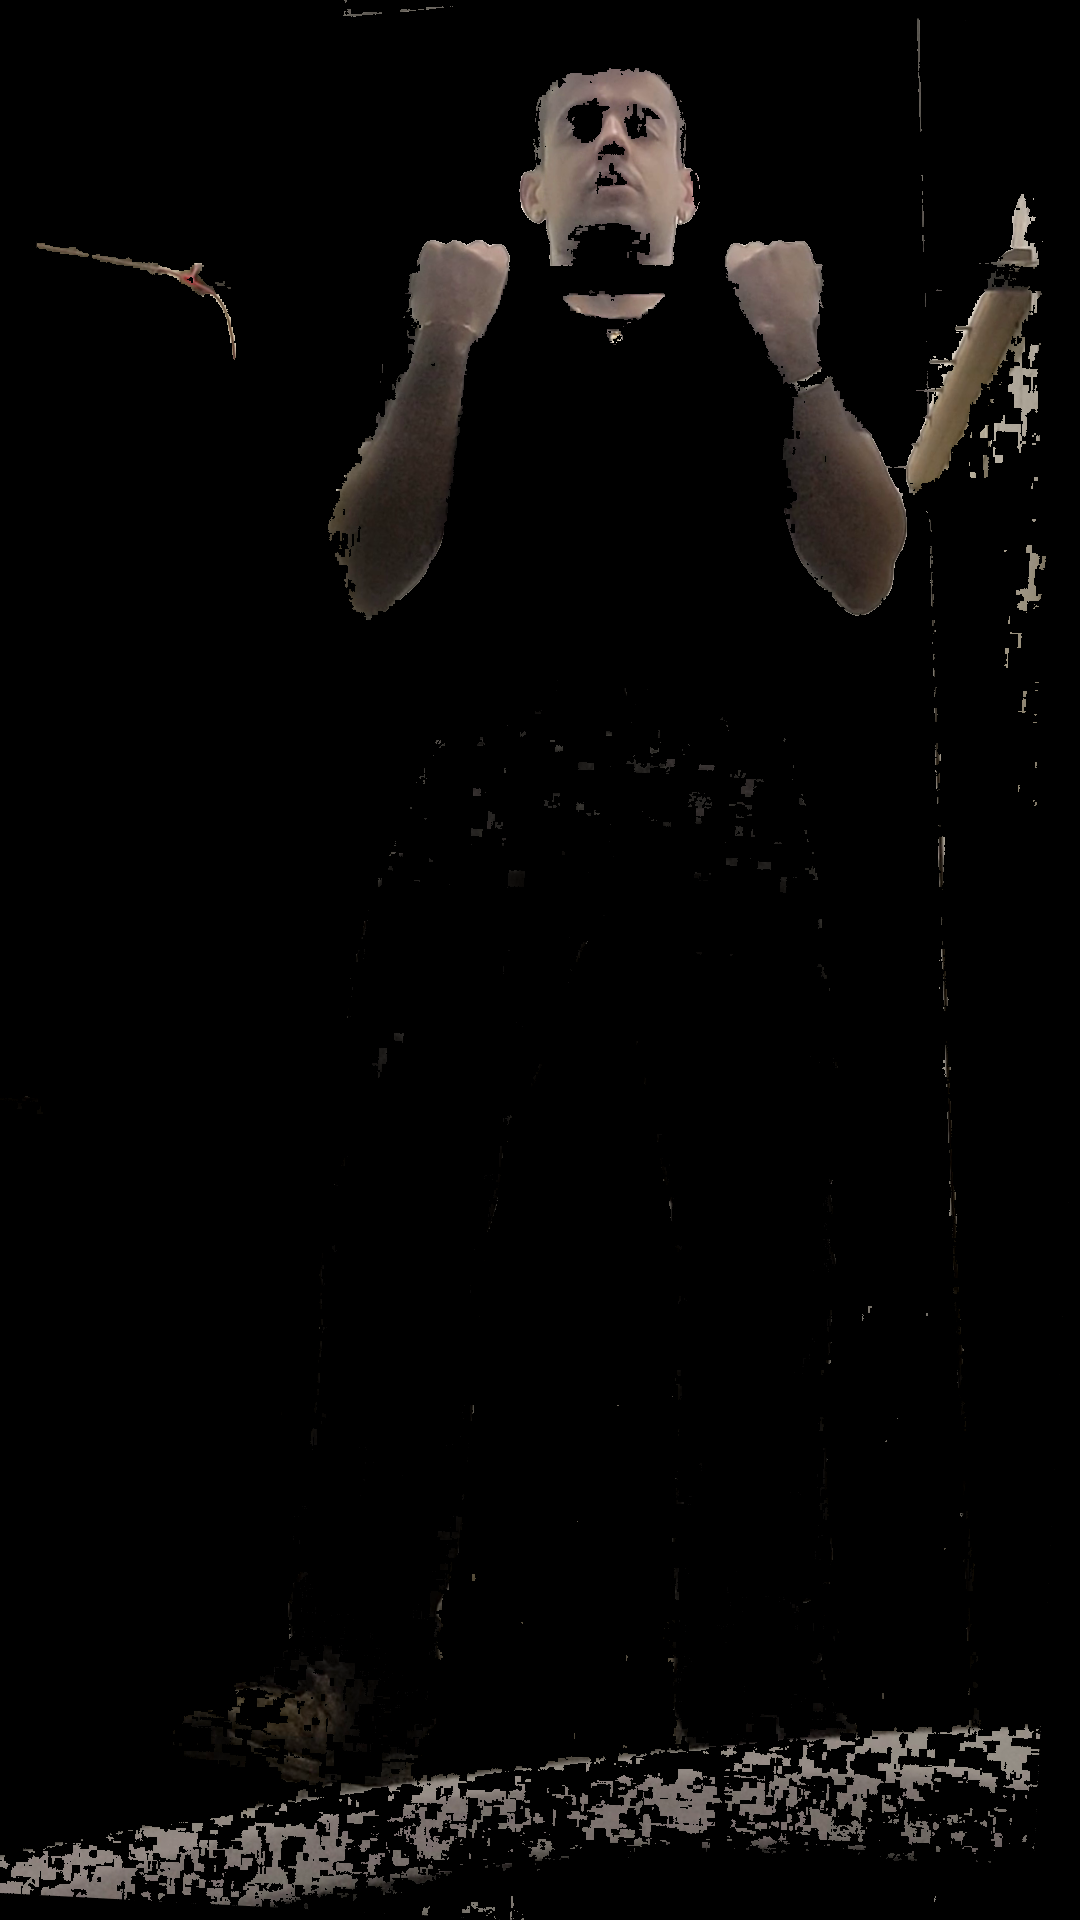
\includegraphics[width=\textwidth]{figuras/ultrapassar_barra/134_skin.png}
        \end{minipage}
\end{figure}
\begin{figure}[H]
    \centering
        \begin{minipage}{\sizeImg\textwidth}
            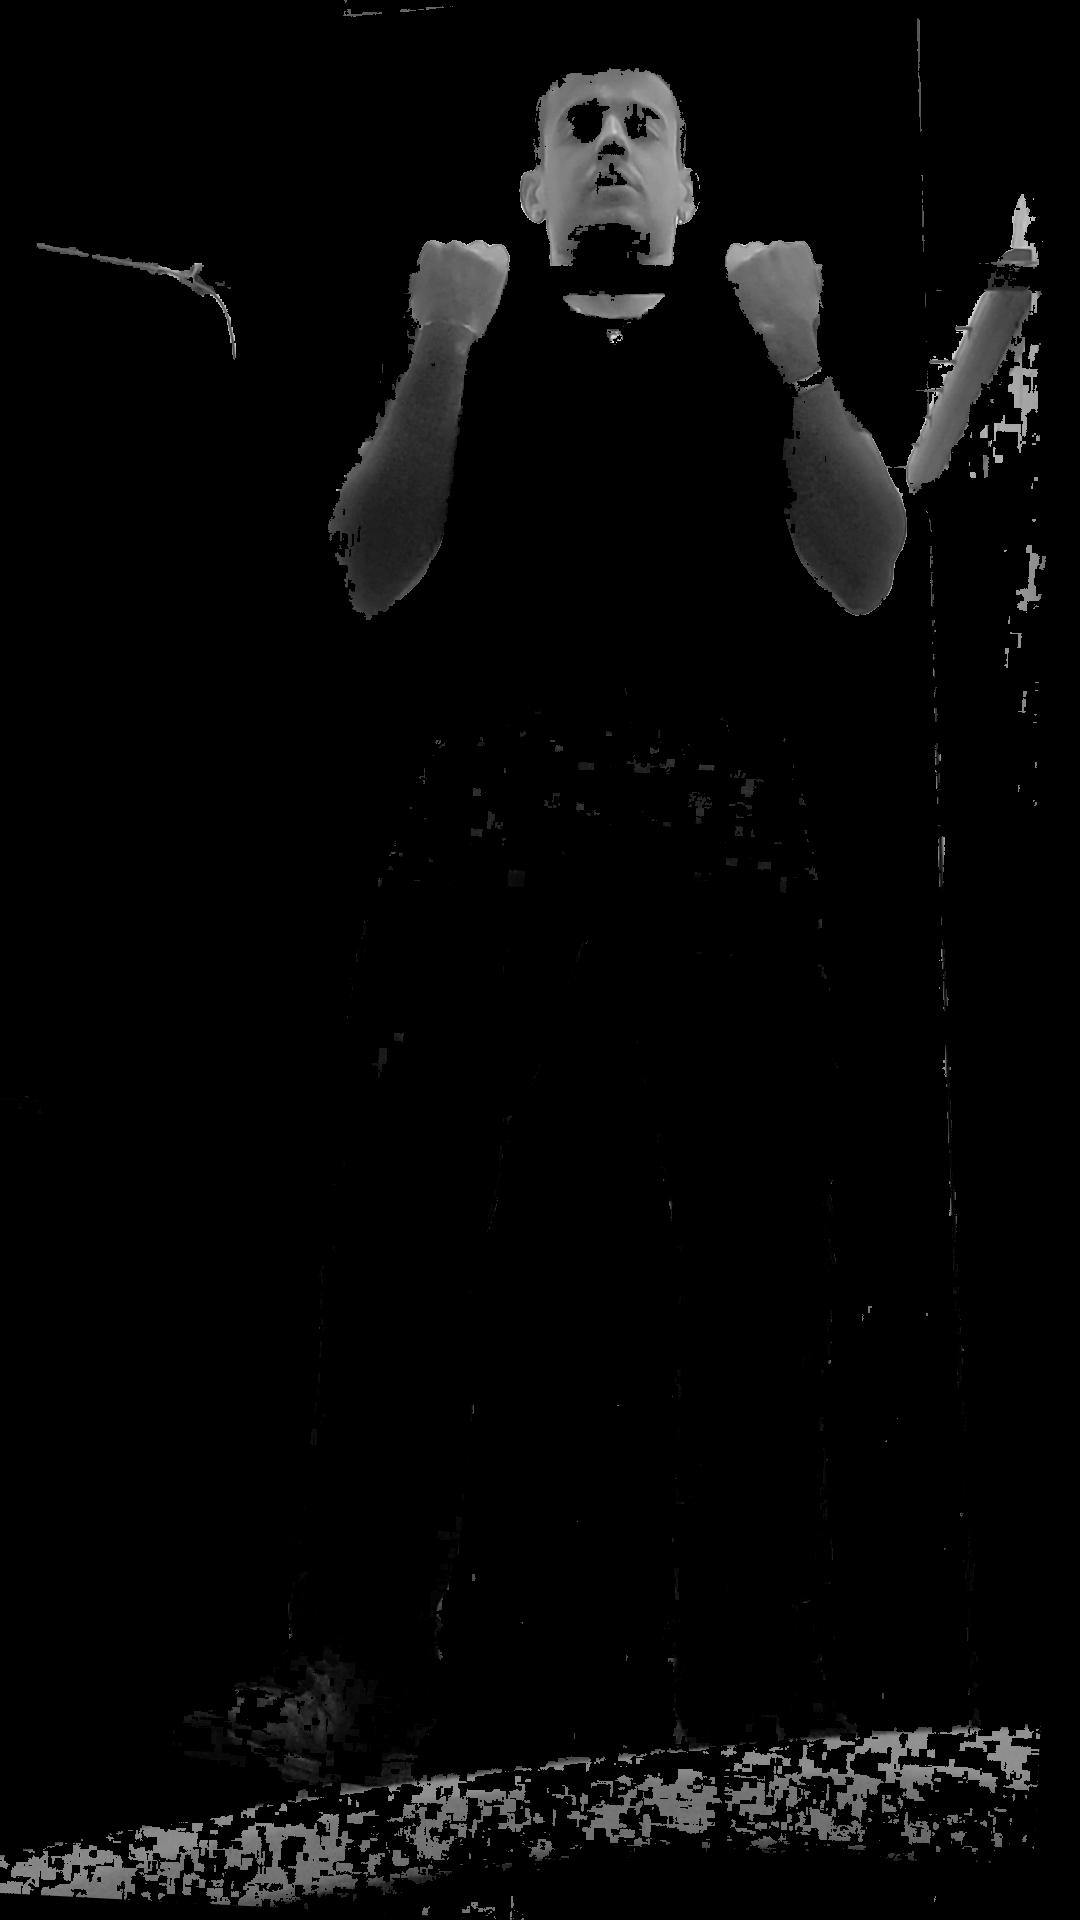
\includegraphics[width=\textwidth]{figuras/ultrapassar_barra/134_gray.png}
        \end{minipage}
        \begin{minipage}{\sizeImg\textwidth}
            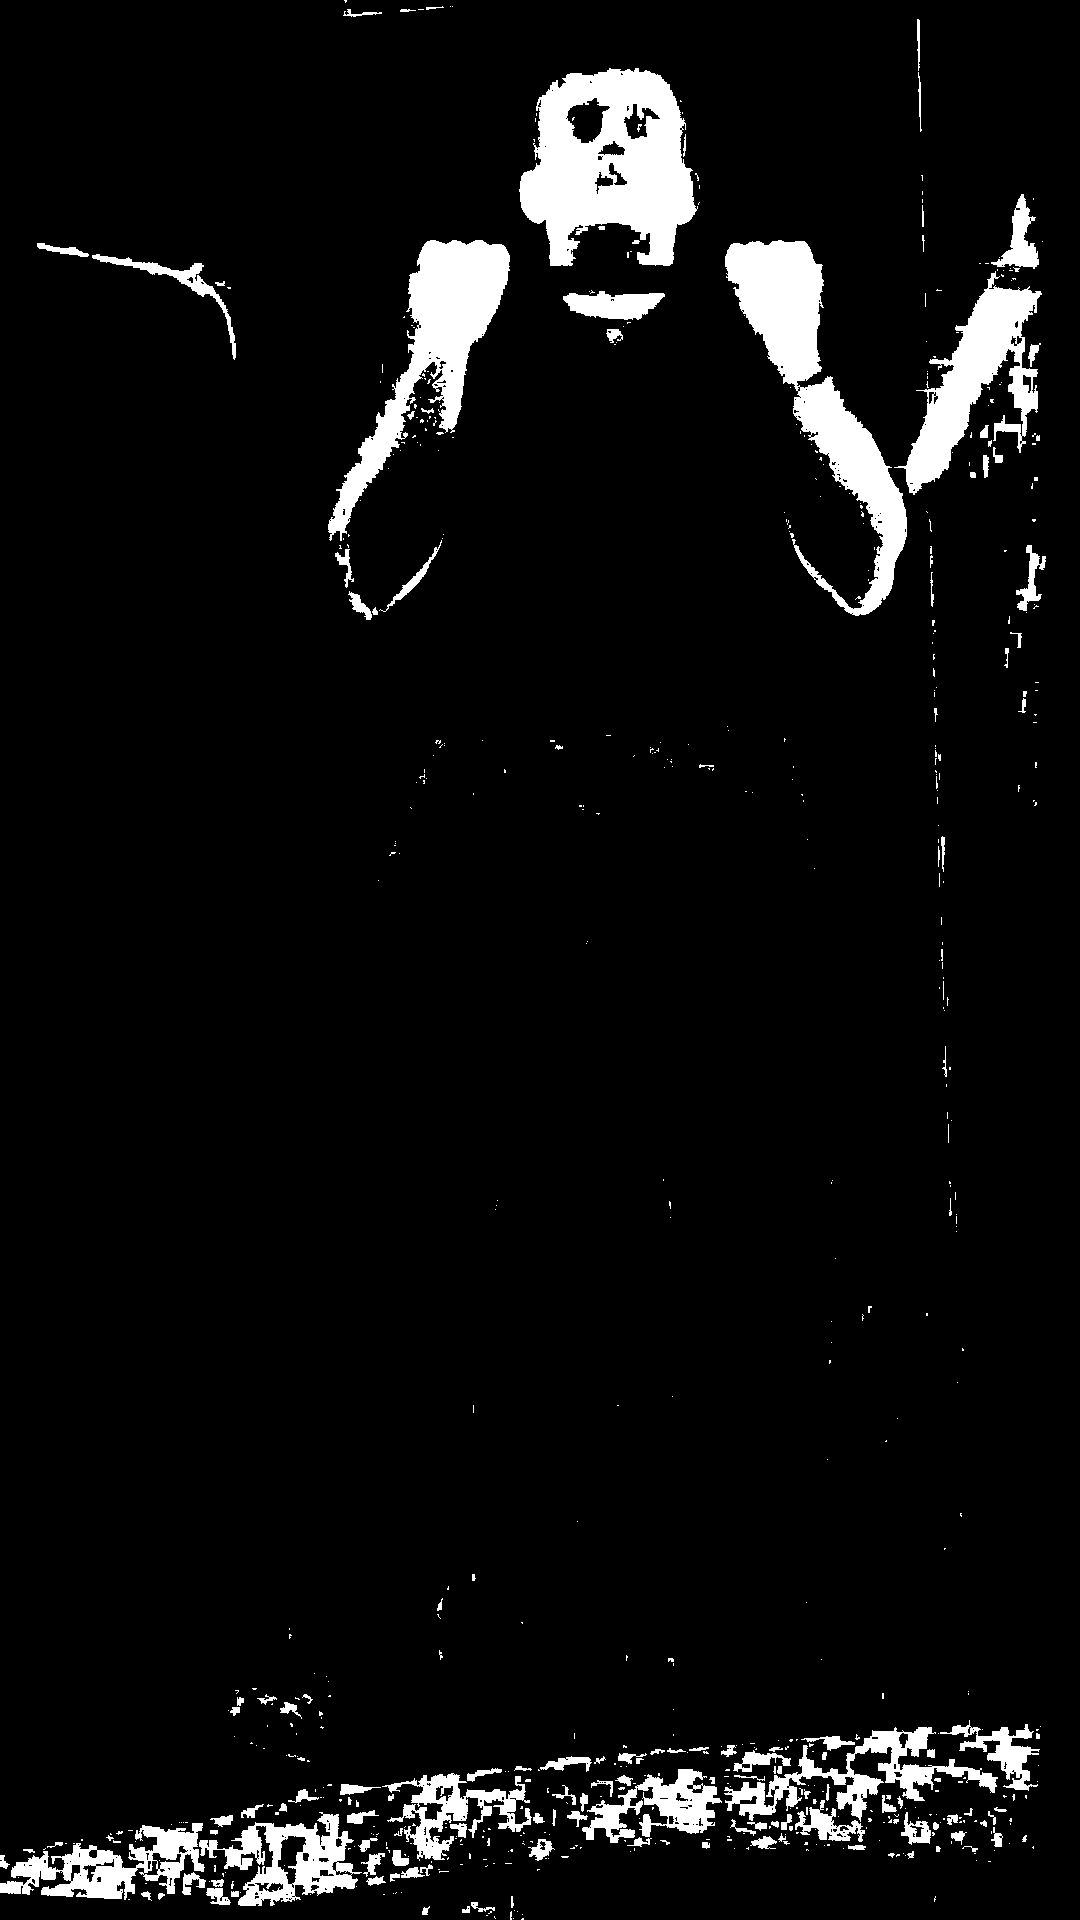
\includegraphics[width=\textwidth]{figuras/ultrapassar_barra/134_limited.png}
        \end{minipage}
    \legend{Fonte: Elaborado pelo autor (2023)}
    \label{fig:bin_ultrapassar_barra}
\end{figure}
\renewcommand{\sizeImg}{0.4}


A partir deste ponto, o processo se destaca, pois é aplicada uma máscara para realçar a região de interesse. As dimensões da máscara são baseadas em um terço da diferença da coordenada $x$ do ombro esquerdo e o ombro direito, com o valor arredondado para baixo, nomeado aqui como $size\_block$. A máscara é definida como um retângulo com a base correspondente a $1,5*(size\_block)$ e altura igual a $(size\_block)/2$, posicionado a uma distância de $1,5*(size\_block)$ da barra, com seu centro alinhado à coordenada $x$ do ponto médio entre o ombro esquerdo e o ombro direito.
 
\begin{figure}[H]
    \centering
    \caption{Representação da mascara para região de interesse }
        \begin{minipage}{\sizeImg\textwidth}
            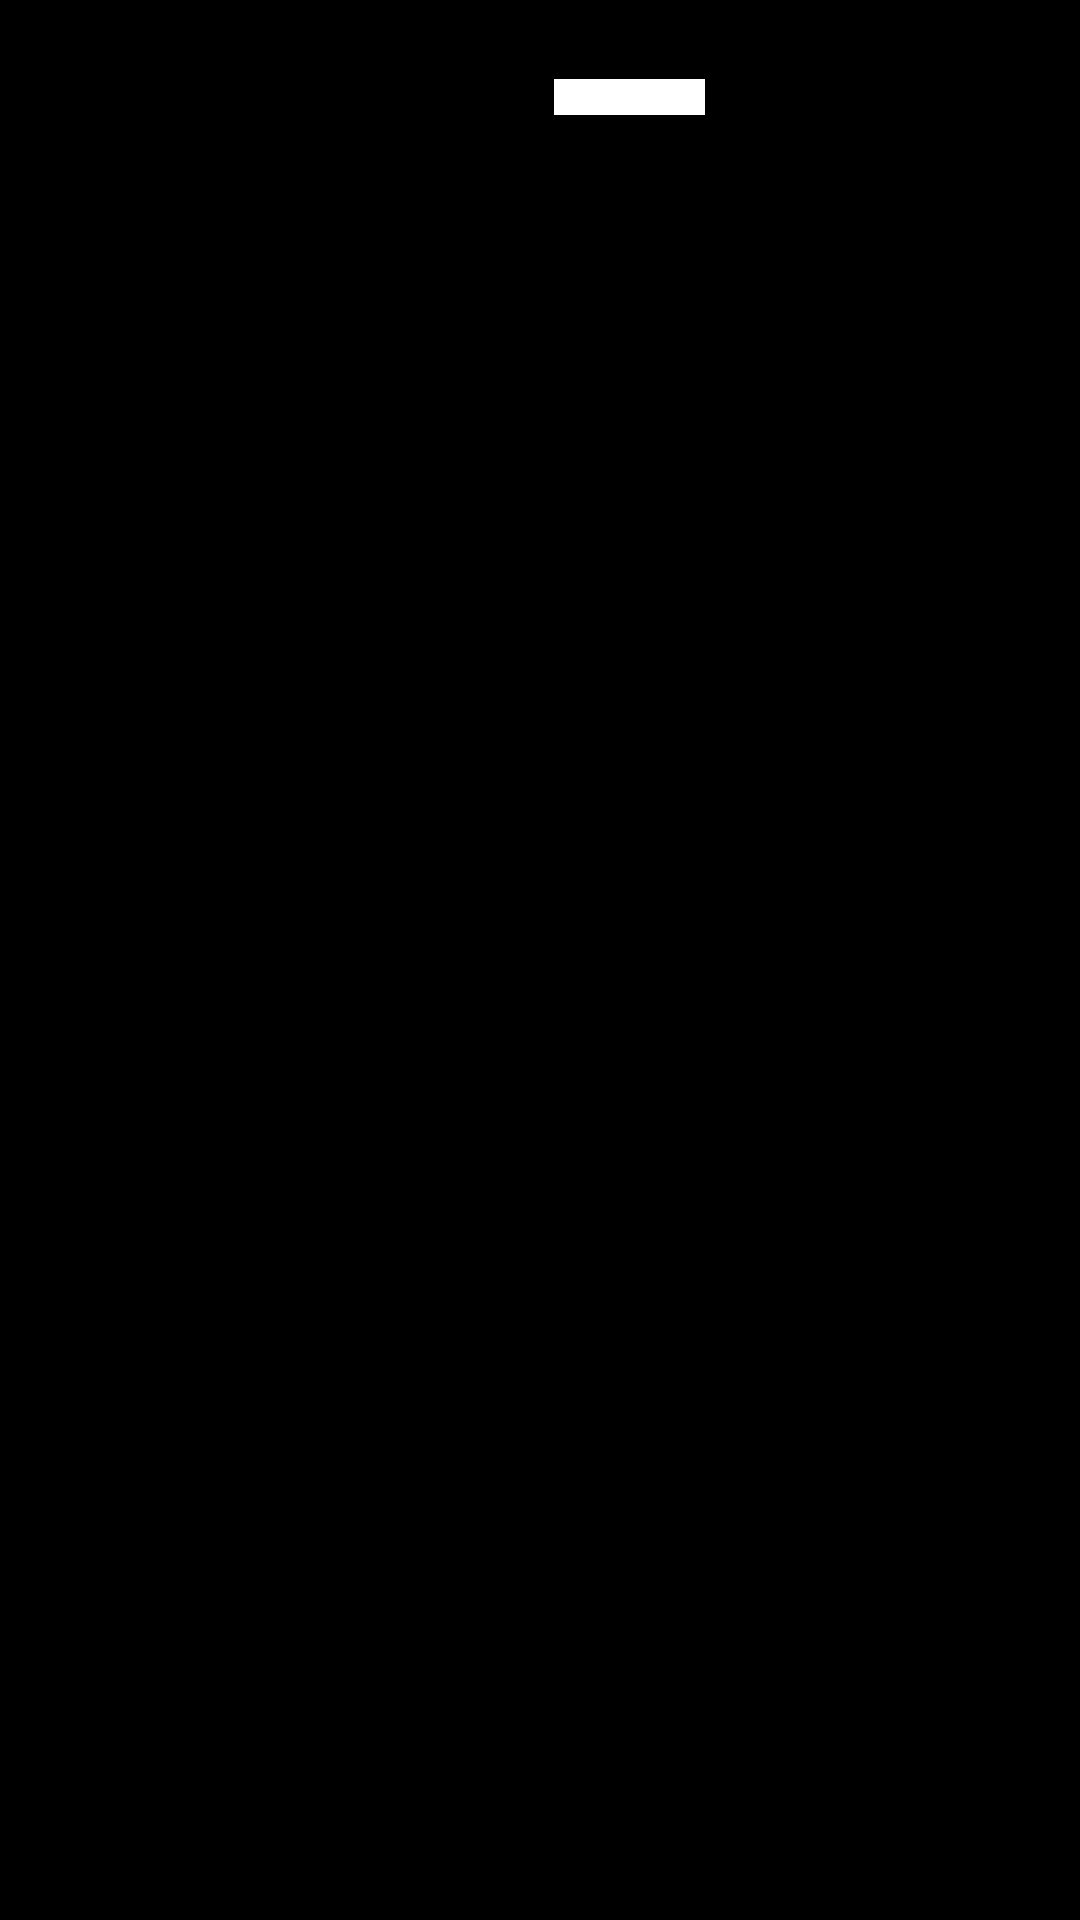
\includegraphics[width=\textwidth]{figuras/ultrapassar_barra/134_mask_head.png}
        \end{minipage}
        \begin{minipage}{\sizeImg\textwidth}
            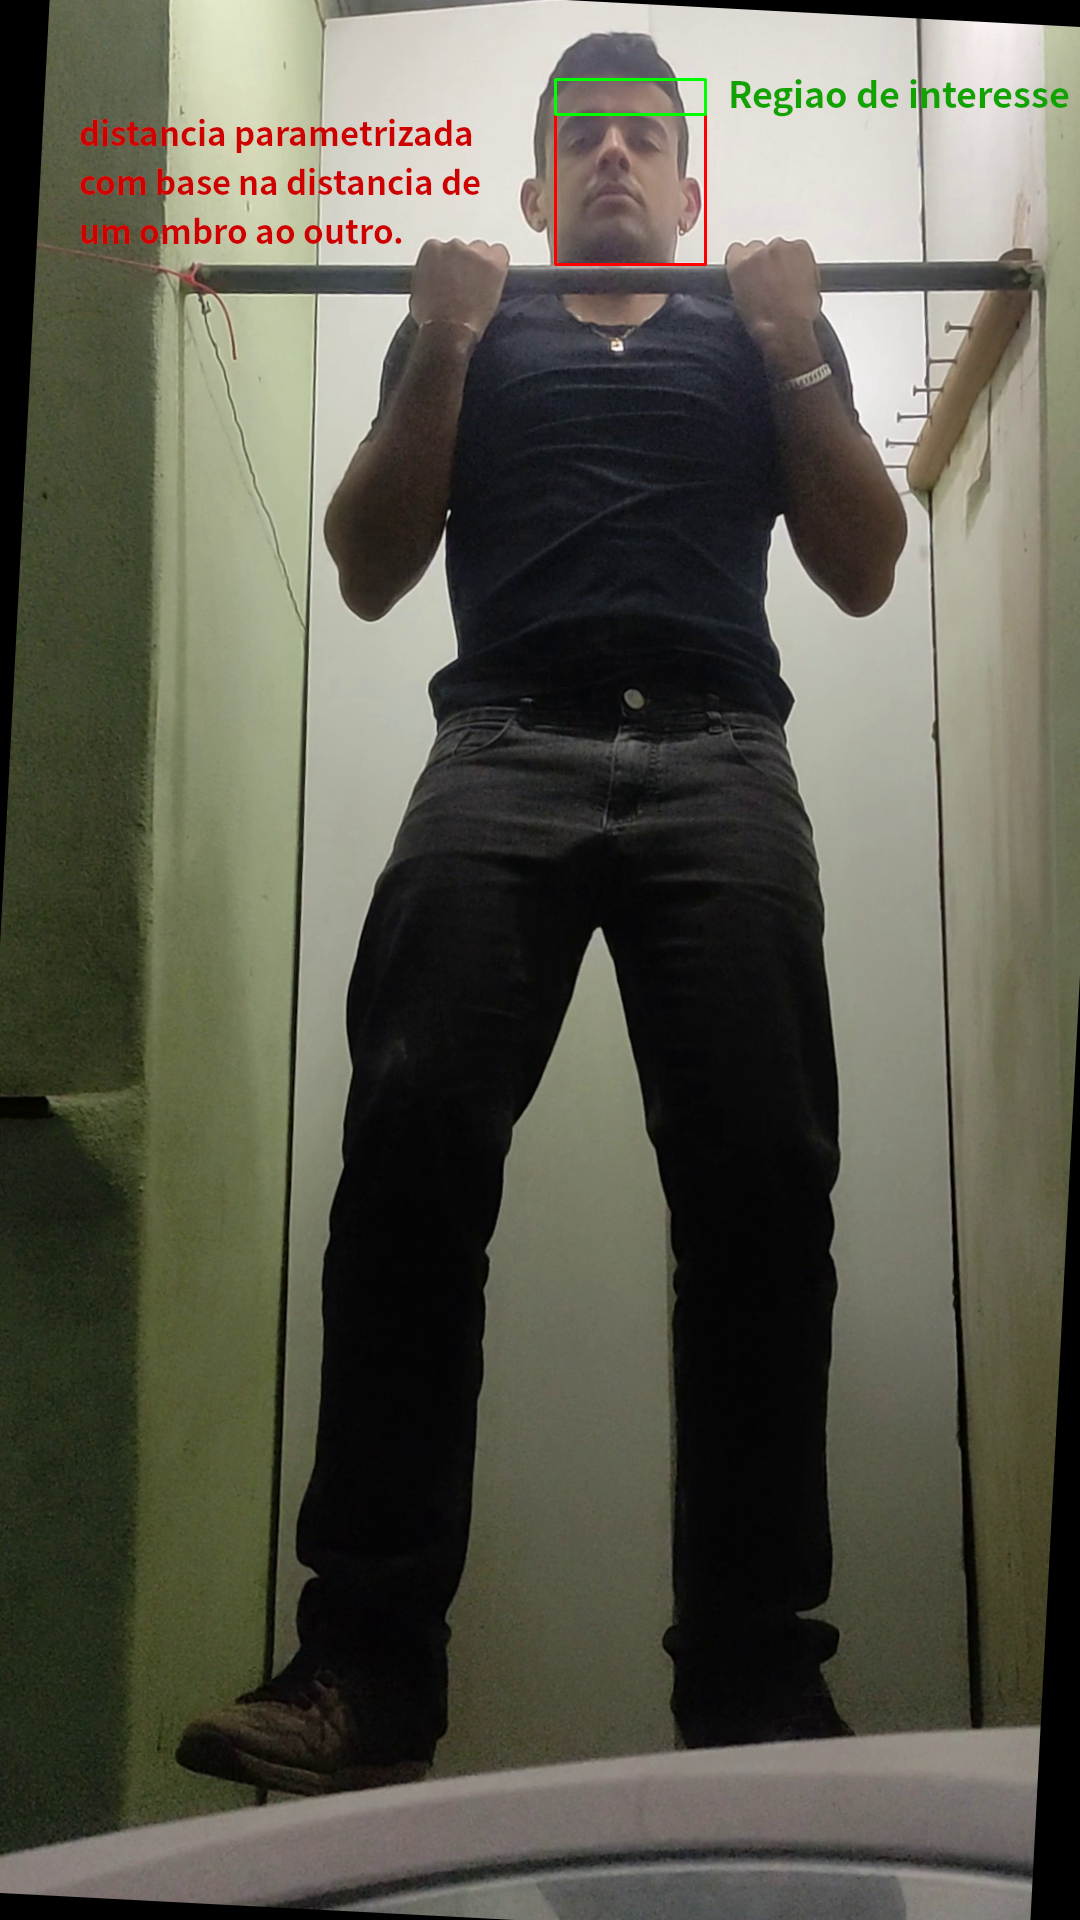
\includegraphics[width=\textwidth]{figuras/ultrapassar_barra/133_image_with_legend.png}
        \end{minipage}
    \legend{Fonte: Elaborado pelo autor (2023)}
    \label{fig:Mascara_ultrapassar_barra}
\end{figure}


Por fim, a detecção de presença na área de interesse é considerada positiva se houver presença de pixels brancos na imagem resultante.

\begin{figure}[H]
	\centering
    \caption{Captura da região de interesse}
	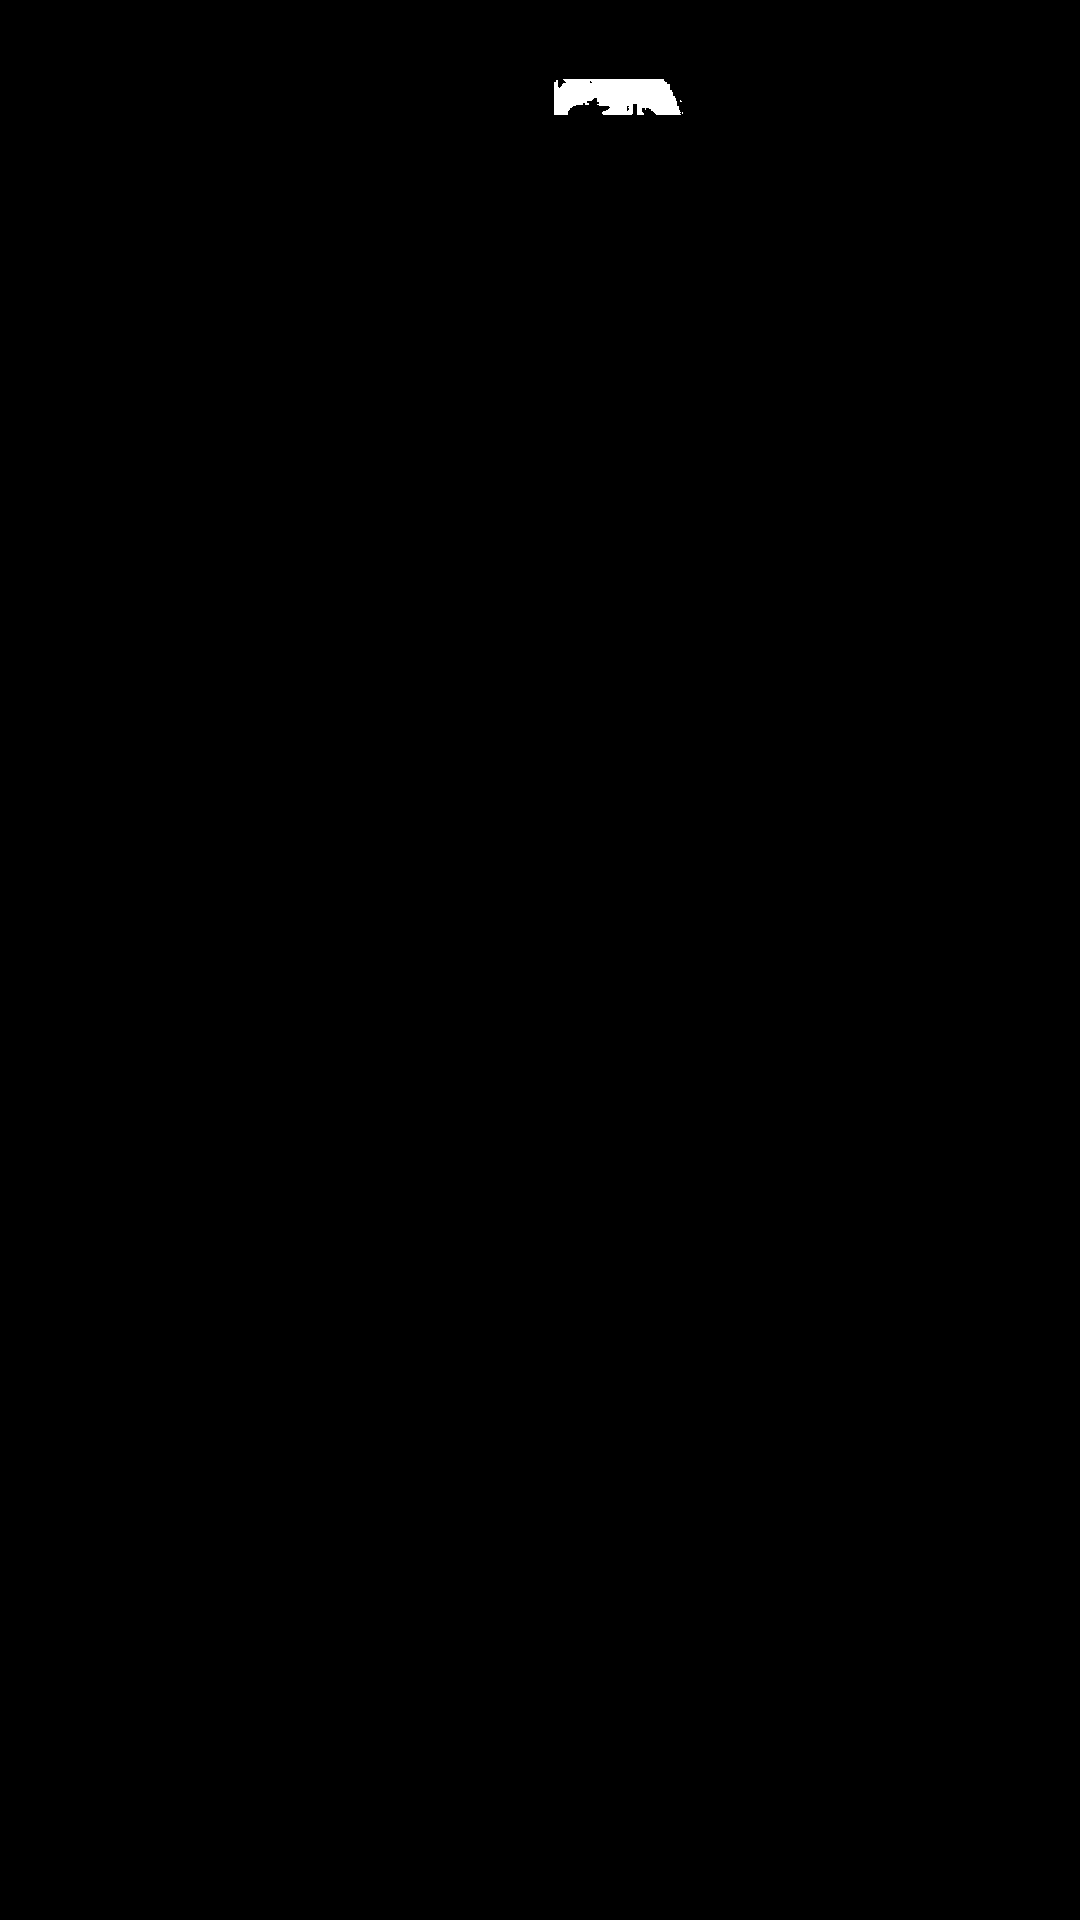
\includegraphics[scale=0.13]{figuras/ultrapassar_barra/134_only_interesse.png}
    \legend{Fonte: Elaborado pelo autor (2023)}
	\label{fig:ultrapassar_barra}
\end{figure}




\subsection[Movimentação do quadril]{Movimentação do quadril}\label{sec:Movimentacao do quadril}

O movimento do quadril foi examinado de maneira semelhante à flexão e extensão do cotovelo; no entanto, os pontos de referência utilizados foram o quadril, o joelho e o tornozelo. A coxa foi considerada como o segmento de linha que se estende do quadril ao joelho, enquanto a perna foi definida como o segmento de linha que se estende do joelho até o tornozelo. Para avaliar a movimentação dos membros inferiores, foi analisado se o ângulo entre os membros, tanto direito quanto esquerdo, excedia 15 graus.





 \section[Codigo fonte]{Codigo fonte}

 O código-fonte pode ser encontrado em um repositório específico hospedado no GitHub. Para acessar e explorar o conjunto completo de arquivos, você pode visitar o seguinte sítio eletrônico: \url{https://github.com/le314u/TCC/tree/main/Tecnologico/Source/Programa/python}. Neste repositório, os arquivos estão organizados de forma a facilitar a navegação e a análise individual de cada componente do programa. Este repositório oferece uma visão abrangente do presente trabalho e é uma valiosa fonte de informações para qualquer pessoa interessada em entender melhor a implementação da ferramenta e queira ter este trabalho como base para trabalhos futuros.
 
 

\subsection[Hierarquia de diretorio]{Hierarquia de diretorio}


O projeto foi estruturado de forma que os componentes do código conseguissem ser divididos em 5 grandes blocos, sendo eles controller, model, view, util e mídia.

\begin{figure}[H]
	\centering
    \caption{Estrutura do diretorio baseado em 5 grande blocos }
	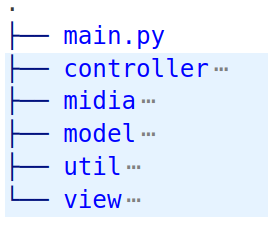
\includegraphics[scale=0.5]{figuras/diretorios/Blocos.png}
    \legend{Fonte: Elaborado pelo autor (2023)}
	\label{fig:blocos}
\end{figure}

No contexto do meu projeto, a estrutura de diretórios é organizada da seguinte forma: o diretório \aspas{model} contém arquivos que desempenham o papel fundamental na representação dos dados e a lógica de negócios da ferramenta.

\begin{figure}[H]
    \centering
    \caption{Estrutura do diretório \aspas{/model}}
    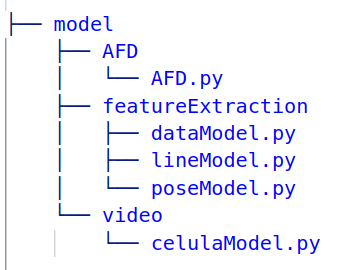
\includegraphics[scale=0.5]{figuras/diretorios/model.png}
    \legend{Fonte: Elaborado pelo autor (2023)}
    \label{fig:model}
\end{figure}



A pasta \aspas{view} é responsável por apresentar esses dados de maneira atraente e interativa aos usuários, assegurando que a interface do usuário reflita com precisão o estado atual do modelo.

\begin{figure}[H]
	\centering
	\caption{Estrutura do diretorio \aspas{/view}}
	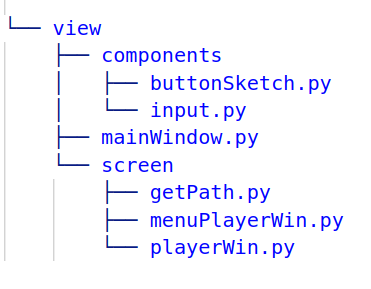
\includegraphics[scale=0.5]{figuras/diretorios/view.png}
    \legend{Fonte: Elaborado pelo autor (2023)}
	\label{fig:view}
\end{figure}

O diretório \aspas{mídia} abriga arquivos relacionados a imagens, áudio, vídeo e às fontes do sistema.

\begin{figure}[H]
	\centering
	\caption{Estrutura do diretorio \aspas{/midia}}
	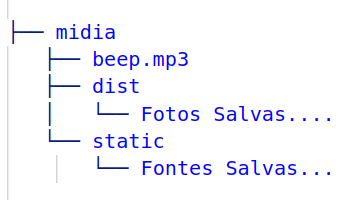
\includegraphics[scale=0.5]{figuras/diretorios/midia.png}
    \legend{Fonte: Elaborado pelo autor (2023)}
	\label{fig:midia}
\end{figure}

Por fim, o diretório \aspas{util} contém arquivos genéricos que não se encaixam especificamente em nenhum desses diretórios e podem ser utilizados em diferentes partes do programa conforme necessário.

\begin{figure}[H]
	\centering
    \caption{Estrutura do diretorio \aspas{/util}}
	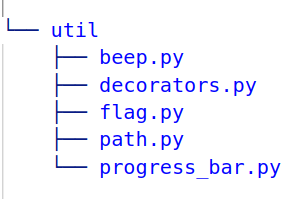
\includegraphics[scale=0.5]{figuras/diretorios/util.png}
    \legend{Fonte: Elaborado pelo autor (2023)}
	\label{fig:util}
\end{figure}

O \aspas{controller} atua como um mediador entre os arquivos da view e do model, interpretando as ações do usuário na interface e coordenando as operações necessárias do model para atender às solicitações, mantendo, assim, uma separação eficaz entre a lógica de apresentação e a lógica de negócios.

\begin{figure}[H]
	\centering
    \caption{Estrutura do diretorio \aspas{/controller}}
	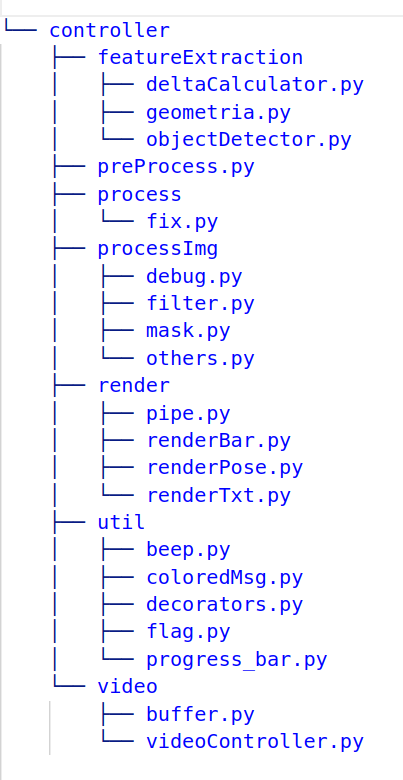
\includegraphics[scale=0.6]{figuras/diretorios/controller.png}
    \legend{Fonte: Elaborado pelo autor (2023)}
	\label{fig:controller}
\end{figure}



\section[Codigo fonte]{Codigo fonte}

O código-fonte pode ser encontrado em um repositório específico hospedado no GitHub. Para acessar e explorar o conjunto completo de arquivos, você pode visitar o seguinte site eletrônico: \url{https://github.com/le314u/TCC/tree/main/Tecnologico/Source/Programa/python}. Neste repositório, os arquivos estão organizados de forma a facilitar a navegação e a análise individual de cada componente do programa. Este repositório oferece uma visão abrangente do presente trabalho e é uma valiosa fonte de informações para qualquer pessoa interessada em entender melhor a implementação da ferramenta e queira ter este trabalho como base para trabalhos futuros.


